\documentclass[twoside]{book}

% Packages required by doxygen
\usepackage{fixltx2e}
\usepackage{calc}
\usepackage{doxygen}
\usepackage[export]{adjustbox} % also loads graphicx
\usepackage{graphicx}
\usepackage[utf8]{inputenc}
\usepackage{makeidx}
\usepackage{multicol}
\usepackage{multirow}
\PassOptionsToPackage{warn}{textcomp}
\usepackage{textcomp}
\usepackage[nointegrals]{wasysym}
\usepackage[table]{xcolor}

% Font selection
\usepackage[T1]{fontenc}
\usepackage[scaled=.90]{helvet}
\usepackage{courier}
\usepackage{amssymb}
\usepackage{sectsty}
\renewcommand{\familydefault}{\sfdefault}
\allsectionsfont{%
  \fontseries{bc}\selectfont%
  \color{darkgray}%
}
\renewcommand{\DoxyLabelFont}{%
  \fontseries{bc}\selectfont%
  \color{darkgray}%
}
\newcommand{\+}{\discretionary{\mbox{\scriptsize$\hookleftarrow$}}{}{}}

% Page & text layout
\usepackage{geometry}
\geometry{%
  a4paper,%
  top=2.5cm,%
  bottom=2.5cm,%
  left=2.5cm,%
  right=2.5cm%
}
\tolerance=750
\hfuzz=15pt
\hbadness=750
\setlength{\emergencystretch}{15pt}
\setlength{\parindent}{0cm}
\setlength{\parskip}{0.2cm}
\makeatletter
\renewcommand{\paragraph}{%
  \@startsection{paragraph}{4}{0ex}{-1.0ex}{1.0ex}{%
    \normalfont\normalsize\bfseries\SS@parafont%
  }%
}
\renewcommand{\subparagraph}{%
  \@startsection{subparagraph}{5}{0ex}{-1.0ex}{1.0ex}{%
    \normalfont\normalsize\bfseries\SS@subparafont%
  }%
}
\makeatother

% Headers & footers
\usepackage{fancyhdr}
\pagestyle{fancyplain}
\fancyhead[LE]{\fancyplain{}{\bfseries\thepage}}
\fancyhead[CE]{\fancyplain{}{}}
\fancyhead[RE]{\fancyplain{}{\bfseries\leftmark}}
\fancyhead[LO]{\fancyplain{}{\bfseries\rightmark}}
\fancyhead[CO]{\fancyplain{}{}}
\fancyhead[RO]{\fancyplain{}{\bfseries\thepage}}
\fancyfoot[LE]{\fancyplain{}{}}
\fancyfoot[CE]{\fancyplain{}{}}
\fancyfoot[RE]{\fancyplain{}{\bfseries\scriptsize Generated on Thu May 28 2015 06\+:05\+:05 for P\+Wlab\+I2 rpg by Doxygen }}
\fancyfoot[LO]{\fancyplain{}{\bfseries\scriptsize Generated on Thu May 28 2015 06\+:05\+:05 for P\+Wlab\+I2 rpg by Doxygen }}
\fancyfoot[CO]{\fancyplain{}{}}
\fancyfoot[RO]{\fancyplain{}{}}
\renewcommand{\footrulewidth}{0.4pt}
\renewcommand{\chaptermark}[1]{%
  \markboth{#1}{}%
}
\renewcommand{\sectionmark}[1]{%
  \markright{\thesection\ #1}%
}

% Indices & bibliography
\usepackage{natbib}
\usepackage[titles]{tocloft}
\setcounter{tocdepth}{3}
\setcounter{secnumdepth}{5}
\makeindex

% Hyperlinks (required, but should be loaded last)
\usepackage{ifpdf}
\ifpdf
  \usepackage[pdftex,pagebackref=true]{hyperref}
\else
  \usepackage[ps2pdf,pagebackref=true]{hyperref}
\fi
\hypersetup{%
  colorlinks=true,%
  linkcolor=blue,%
  citecolor=blue,%
  unicode%
}

% Custom commands
\newcommand{\clearemptydoublepage}{%
  \newpage{\pagestyle{empty}\cleardoublepage}%
}


%===== C O N T E N T S =====

\begin{document}

% Titlepage & ToC
\hypersetup{pageanchor=false,
             bookmarks=true,
             bookmarksnumbered=true,
             pdfencoding=unicode
            }
\pagenumbering{roman}
\begin{titlepage}
\vspace*{7cm}
\begin{center}%
{\Large P\+Wlab\+I2 rpg }\\
\vspace*{1cm}
{\large Generated by Doxygen 1.8.9.1}\\
\vspace*{0.5cm}
{\small Thu May 28 2015 06:05:05}\\
\end{center}
\end{titlepage}
\clearemptydoublepage
\tableofcontents
\clearemptydoublepage
\pagenumbering{arabic}
\hypersetup{pageanchor=true}

%--- Begin generated contents ---
\chapter{Hierarchical Index}
\section{Class Hierarchy}
This inheritance list is sorted roughly, but not completely, alphabetically\+:\begin{DoxyCompactList}
\item \contentsline{section}{Array$<$ T\+Y\+P\+E $>$}{\pageref{classArray}}{}
\item \contentsline{section}{Array$<$ Vector\+X\+Y $\ast$ $>$}{\pageref{classArray}}{}
\item \contentsline{section}{Base\+Event}{\pageref{classBaseEvent}}{}
\begin{DoxyCompactList}
\item \contentsline{section}{Event$<$ D $>$}{\pageref{classEvent}}{}
\end{DoxyCompactList}
\item \contentsline{section}{Chain$<$ T\+Y\+P\+E $>$}{\pageref{classChain}}{}
\item \contentsline{section}{Chain$<$ char $>$}{\pageref{classChain}}{}
\item \contentsline{section}{Chain$<$ const char $\ast$ $>$}{\pageref{classChain}}{}
\item \contentsline{section}{Chain$<$ Game\+Session \& $>$}{\pageref{classChain}}{}
\item \contentsline{section}{Chain$<$ Object\+Map\+Meta \& $>$}{\pageref{classChain}}{}
\item \contentsline{section}{Chain$<$ Object\+Physics\+Meta $\ast$ $>$}{\pageref{classChain}}{}
\item \contentsline{section}{Chain$<$ Physics\+Engine\+:\+:Collision\+Grid\+:\+:Grid\+Pool $\ast$ $>$}{\pageref{classChain}}{}
\item \contentsline{section}{Chain$<$ Physics\+Engine\+:\+:C\+R\+Ent $>$}{\pageref{classChain}}{}
\item \contentsline{section}{Chain$<$ Team $>$}{\pageref{classChain}}{}
\item \contentsline{section}{Physics\+Engine\+:\+:Collision\+Grid}{\pageref{classPhysicsEngine_1_1CollisionGrid}}{}
\item \contentsline{section}{Physics\+Engine\+:\+:C\+R\+Ent}{\pageref{structPhysicsEngine_1_1CREnt}}{}
\item \contentsline{section}{Decal}{\pageref{classDecal}}{}
\begin{DoxyCompactList}
\item \contentsline{section}{Object}{\pageref{classObject}}{}
\begin{DoxyCompactList}
\item \contentsline{section}{Actor}{\pageref{classActor}}{}
\begin{DoxyCompactList}
\item \contentsline{section}{Player}{\pageref{classPlayer}}{}
\end{DoxyCompactList}
\item \contentsline{section}{Grass}{\pageref{classGrass}}{}
\item \contentsline{section}{Health\+Bar}{\pageref{classHealthBar}}{}
\item \contentsline{section}{Tree}{\pageref{classTree}}{}
\end{DoxyCompactList}
\end{DoxyCompactList}
\item \contentsline{section}{Game\+Domain}{\pageref{classGameDomain}}{}
\item \contentsline{section}{Game\+Engine}{\pageref{classGameEngine}}{}
\item \contentsline{section}{Game\+Map}{\pageref{classGameMap}}{}
\item \contentsline{section}{Game\+Session}{\pageref{classGameSession}}{}
\item \contentsline{section}{G\+C\+Ref}{\pageref{classGCRef}}{}
\begin{DoxyCompactList}
\item \contentsline{section}{Interface}{\pageref{classInterface}}{}
\begin{DoxyCompactList}
\item \contentsline{section}{Engine\+Start}{\pageref{classEngineStart}}{}
\item \contentsline{section}{Intro}{\pageref{classIntro}}{}
\item \contentsline{section}{Player\+Controller}{\pageref{classPlayerController}}{}
\end{DoxyCompactList}
\item \contentsline{section}{Object}{\pageref{classObject}}{}
\item \contentsline{section}{Object\+Map\+Meta}{\pageref{classObjectMapMeta}}{}
\begin{DoxyCompactList}
\item \contentsline{section}{Object\+Physics\+Meta}{\pageref{classObjectPhysicsMeta}}{}
\end{DoxyCompactList}
\end{DoxyCompactList}
\item \contentsline{section}{G\+C\+Ref\+Link}{\pageref{classGCRefLink}}{}
\item \contentsline{section}{Physics\+Engine\+:\+:Collision\+Grid\+:\+:Grid\+Pool}{\pageref{structPhysicsEngine_1_1CollisionGrid_1_1GridPool}}{}
\item \contentsline{section}{Light\+Source}{\pageref{classLightSource}}{}
\begin{DoxyCompactList}
\item \contentsline{section}{Object}{\pageref{classObject}}{}
\end{DoxyCompactList}
\item \contentsline{section}{Render\+Engine\+:\+:obj\+Record}{\pageref{structRenderEngine_1_1objRecord}}{}
\item \contentsline{section}{Physical\+Body}{\pageref{classPhysicalBody}}{}
\begin{DoxyCompactList}
\item \contentsline{section}{Object}{\pageref{classObject}}{}
\end{DoxyCompactList}
\item \contentsline{section}{Physics\+Engine}{\pageref{classPhysicsEngine}}{}
\item \contentsline{section}{Point\+X\+Y}{\pageref{classPointXY}}{}
\item \contentsline{section}{Render\+Engine}{\pageref{classRenderEngine}}{}
\item \contentsline{section}{Timer}{\pageref{classTimer}}{}
\item \contentsline{section}{Typed\+Class}{\pageref{classTypedClass}}{}
\begin{DoxyCompactList}
\item \contentsline{section}{Object}{\pageref{classObject}}{}
\item \contentsline{section}{Object\+Map\+Meta}{\pageref{classObjectMapMeta}}{}
\end{DoxyCompactList}
\item \contentsline{section}{Vector\+X\+Y}{\pageref{classVectorXY}}{}
\end{DoxyCompactList}

\chapter{Class Index}
\section{Class List}
Here are the classes, structs, unions and interfaces with brief descriptions\+:\begin{DoxyCompactList}
\item\contentsline{section}{\hyperlink{classActor}{Actor} }{\pageref{classActor}}{}
\item\contentsline{section}{\hyperlink{classArray}{Array$<$ T\+Y\+P\+E $>$} \\*\hyperlink{classArray}{Array} class providing some common operations on tables }{\pageref{classArray}}{}
\item\contentsline{section}{\hyperlink{classBaseEvent}{Base\+Event} \\*Class providing events functionality designed for session management }{\pageref{classBaseEvent}}{}
\item\contentsline{section}{\hyperlink{classChain}{Chain$<$ T\+Y\+P\+E $>$} \\*\hyperlink{classChain}{Chain} class providing bi-\/directional-\/list like data organisation }{\pageref{classChain}}{}
\item\contentsline{section}{\hyperlink{classPhysicsEngine_1_1CollisionGrid}{Physics\+Engine\+::\+Collision\+Grid} \\*Class containing collision grid for optimization purpose }{\pageref{classPhysicsEngine_1_1CollisionGrid}}{}
\item\contentsline{section}{\hyperlink{structPhysicsEngine_1_1CREnt}{Physics\+Engine\+::\+C\+R\+Ent} }{\pageref{structPhysicsEngine_1_1CREnt}}{}
\item\contentsline{section}{\hyperlink{classDecal}{Decal} \\*Renderable \hyperlink{classDecal}{Decal} for Render Engine }{\pageref{classDecal}}{}
\item\contentsline{section}{\hyperlink{classEngineStart}{Engine\+Start} }{\pageref{classEngineStart}}{}
\item\contentsline{section}{\hyperlink{classEvent}{Event$<$ D $>$} \\*The \hyperlink{classEvent}{Event} class extension to \hyperlink{classBaseEvent}{Base\+Event} class allowing drivers to pass custom data in event }{\pageref{classEvent}}{}
\item\contentsline{section}{\hyperlink{classGameDomain}{Game\+Domain} \\*Game domain manager class, providing game domain code layer for game logic }{\pageref{classGameDomain}}{}
\item\contentsline{section}{\hyperlink{classGameEngine}{Game\+Engine} \\*Main game engine class }{\pageref{classGameEngine}}{}
\item\contentsline{section}{\hyperlink{classGameMap}{Game\+Map} \\*Map class }{\pageref{classGameMap}}{}
\item\contentsline{section}{\hyperlink{classGameSession}{Game\+Session} \\*Base game engine class providing session functionality }{\pageref{classGameSession}}{}
\item\contentsline{section}{\hyperlink{classGCRef}{G\+C\+Ref} \\*Class providing basic garbage collecting functionality similar to one provided by sharedptr }{\pageref{classGCRef}}{}
\item\contentsline{section}{\hyperlink{classGCRefLink}{G\+C\+Ref\+Link} \\*Helper class to \hyperlink{classGCRefLink}{G\+C\+Ref\+Link}, once deleted -\/ \hyperlink{classGCRef}{G\+C\+Ref} class will unbind reference user and if it was last reference -\/ delete data }{\pageref{classGCRefLink}}{}
\item\contentsline{section}{\hyperlink{classGrass}{Grass} }{\pageref{classGrass}}{}
\item\contentsline{section}{\hyperlink{structPhysicsEngine_1_1CollisionGrid_1_1GridPool}{Physics\+Engine\+::\+Collision\+Grid\+::\+Grid\+Pool} \\*$<$ grid pool entry }{\pageref{structPhysicsEngine_1_1CollisionGrid_1_1GridPool}}{}
\item\contentsline{section}{\hyperlink{classInterface}{Interface} \\*\hyperlink{classInterface}{Interface} to be implemented by all drivers }{\pageref{classInterface}}{}
\item\contentsline{section}{\hyperlink{classIntro}{Intro} }{\pageref{classIntro}}{}
\item\contentsline{section}{\hyperlink{classLightSource}{Light\+Source} \\*Unimplemented }{\pageref{classLightSource}}{}
\item\contentsline{section}{\hyperlink{classObject}{Object} \\*Basic object class }{\pageref{classObject}}{}
\item\contentsline{section}{\hyperlink{classObjectMapMeta}{Object\+Map\+Meta} \\*\hyperlink{classObject}{Object} meta class containing map-\/related properties of object }{\pageref{classObjectMapMeta}}{}
\item\contentsline{section}{\hyperlink{classObjectPhysicsMeta}{Object\+Physics\+Meta} \\*Extension to \hyperlink{classObjectMapMeta}{Object\+Map\+Meta} class adding physical properties like speed, acceleration.. }{\pageref{classObjectPhysicsMeta}}{}
\item\contentsline{section}{\hyperlink{structRenderEngine_1_1objRecord}{Render\+Engine\+::obj\+Record} }{\pageref{structRenderEngine_1_1objRecord}}{}
\item\contentsline{section}{\hyperlink{classPhysicalBody}{Physical\+Body} \\*Class providing basic physical capabilities }{\pageref{classPhysicalBody}}{}
\item\contentsline{section}{\hyperlink{classPhysicsEngine}{Physics\+Engine} \\*Class providing basic physics functionality to registered map }{\pageref{classPhysicsEngine}}{}
\item\contentsline{section}{\hyperlink{classPlayer}{Player} }{\pageref{classPlayer}}{}
\item\contentsline{section}{\hyperlink{classPlayerController}{Player\+Controller} }{\pageref{classPlayerController}}{}
\item\contentsline{section}{\hyperlink{classPointXY}{Point\+X\+Y} \\*Class providing basic point functionality }{\pageref{classPointXY}}{}
\item\contentsline{section}{\hyperlink{classRenderEngine}{Render\+Engine} \\*Rendering engine for game }{\pageref{classRenderEngine}}{}
\item\contentsline{section}{\hyperlink{classTimer}{Timer} \\*\hyperlink{classTimer}{Timer} class providing timer functionality, can be used to generate signal with certain frequency }{\pageref{classTimer}}{}
\item\contentsline{section}{\hyperlink{classTree}{Tree} }{\pageref{classTree}}{}
\item\contentsline{section}{\hyperlink{classTypedClass}{Typed\+Class} \\*Class meant to be inherited by classes meant to be downcasted, providing basic \char`\"{}instanceof\char`\"{} functionality }{\pageref{classTypedClass}}{}
\item\contentsline{section}{\hyperlink{classVectorXY}{Vector\+X\+Y} \\*Class providing basic vector functionality }{\pageref{classVectorXY}}{}
\end{DoxyCompactList}

\chapter{Class Documentation}
\hypertarget{classActor}{}\section{Actor Class Reference}
\label{classActor}\index{Actor@{Actor}}


The \hyperlink{classActor}{Actor} class is a parent class for \hyperlink{classPlayer}{Player},Npc et cetera.  




{\ttfamily \#include $<$Actor.\+h$>$}

Inheritance diagram for Actor\+:\begin{figure}[H]
\begin{center}
\leavevmode
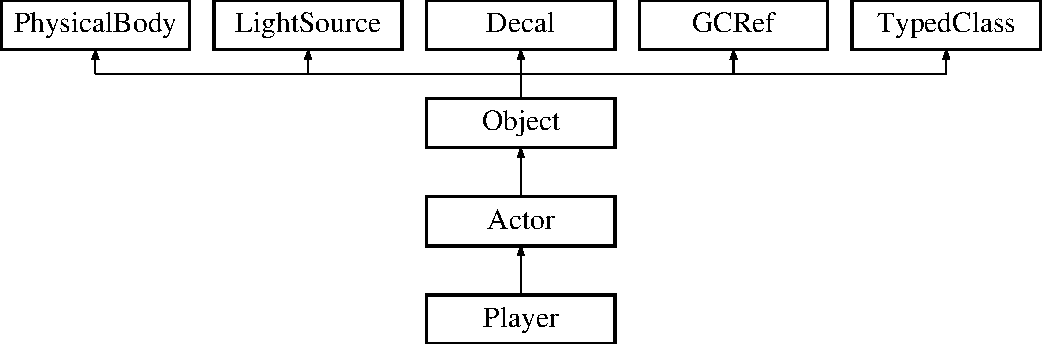
\includegraphics[height=4.000000cm]{classActor}
\end{center}
\end{figure}
\subsection*{Public Member Functions}
\begin{DoxyCompactItemize}
\item 
\hypertarget{classActor_aaa8c3a626ddda737270006259be1bfbe}{}{\bfseries Actor} (std\+::string n=\char`\"{}Actor\char`\"{}, float maxhp=1, float curhp=1, int lvl=1)\label{classActor_aaa8c3a626ddda737270006259be1bfbe}

\item 
\hypertarget{classActor_a162b1257ffca028edd0d4db0077cf671}{}void \hyperlink{classActor_a162b1257ffca028edd0d4db0077cf671}{set\+Max\+Health\+Point} (float mhp)\label{classActor_a162b1257ffca028edd0d4db0077cf671}

\begin{DoxyCompactList}\small\item\em thanks to that we can set a class variable Max\+Health\+Point \end{DoxyCompactList}\item 
\hypertarget{classActor_a12e31ce9c3517bd08640d7cc6b1748d8}{}void \hyperlink{classActor_a12e31ce9c3517bd08640d7cc6b1748d8}{set\+Current\+Health\+Point} (float curhp)\label{classActor_a12e31ce9c3517bd08640d7cc6b1748d8}

\begin{DoxyCompactList}\small\item\em thanks to that we can set a class variable Current\+Health\+Point \end{DoxyCompactList}\item 
\hypertarget{classActor_a771a4d2caa4cb8332b18f8bd6f786245}{}void \hyperlink{classActor_a771a4d2caa4cb8332b18f8bd6f786245}{set\+Level} (int lvl)\label{classActor_a771a4d2caa4cb8332b18f8bd6f786245}

\begin{DoxyCompactList}\small\item\em thanks to that we can set a class variable Level \end{DoxyCompactList}\item 
\hypertarget{classActor_ab8df0b5c89a00f84095977cdb34029c7}{}float \hyperlink{classActor_ab8df0b5c89a00f84095977cdb34029c7}{get\+Max\+Health\+Point} () const \label{classActor_ab8df0b5c89a00f84095977cdb34029c7}

\begin{DoxyCompactList}\small\item\em That function help us to see what is in class variable Max\+Health\+Point. \end{DoxyCompactList}\item 
\hypertarget{classActor_a09fbcbbca7b72174ba9fb5af36c3d9f2}{}float \hyperlink{classActor_a09fbcbbca7b72174ba9fb5af36c3d9f2}{get\+Current\+Health\+Point} () const \label{classActor_a09fbcbbca7b72174ba9fb5af36c3d9f2}

\begin{DoxyCompactList}\small\item\em That function help us to see what is in class variable Current\+Health\+Point. \end{DoxyCompactList}\item 
\hypertarget{classActor_ae42874679e670febffa8919497a4fddd}{}int \hyperlink{classActor_ae42874679e670febffa8919497a4fddd}{get\+Level} () const \label{classActor_ae42874679e670febffa8919497a4fddd}

\begin{DoxyCompactList}\small\item\em That function help us to see what is in class variable Current\+Health\+Point. \end{DoxyCompactList}\end{DoxyCompactItemize}
\subsection*{Static Public Attributes}
\begin{DoxyCompactItemize}
\item 
\hypertarget{classActor_a9499766a969b46ad8336d5ae00712fa2}{}static constexpr char $\ast$ \hyperlink{classActor_a9499766a969b46ad8336d5ae00712fa2}{type\+Name} =(char$\ast$)\char`\"{}Actor\char`\"{}\label{classActor_a9499766a969b46ad8336d5ae00712fa2}

\begin{DoxyCompactList}\small\item\em This help us to recognise later a type of \hyperlink{classObject}{Object}. \end{DoxyCompactList}\end{DoxyCompactItemize}
\subsection*{Additional Inherited Members}


\subsection{Detailed Description}
The \hyperlink{classActor}{Actor} class is a parent class for \hyperlink{classPlayer}{Player},Npc et cetera. 

This class help us with creating a \hyperlink{classObject}{Object} Class with something new. Class contain some basic attributes for actor characters.

\begin{DoxySeeAlso}{See also}
\hyperlink{classObject}{Object} 

\hyperlink{classPlayer}{Player} 
\end{DoxySeeAlso}


The documentation for this class was generated from the following files\+:\begin{DoxyCompactItemize}
\item 
drivers/include/Actor.\+h\item 
drivers/src/Actor.\+cpp\end{DoxyCompactItemize}

\hypertarget{classArray}{}\section{Array$<$ T\+Y\+P\+E $>$ Class Template Reference}
\label{classArray}\index{Array$<$ T\+Y\+P\+E $>$@{Array$<$ T\+Y\+P\+E $>$}}


\hyperlink{classArray}{Array} class providing some common operations on tables.  




{\ttfamily \#include $<$misc.\+h$>$}

\subsection*{Public Member Functions}
\begin{DoxyCompactItemize}
\item 
\hyperlink{classArray_ae135878c586419c57baf3edf7fa0fe21}{Array} (int \hyperlink{classArray_a3a088222b444a20f1d926ee7b44fa868}{length})
\begin{DoxyCompactList}\small\item\em \hyperlink{classArray}{Array} \hyperlink{classArray}{Array} constructor. \end{DoxyCompactList}\item 
\hyperlink{classArray_a9307cd54f769f06cd738443f3ddaeb0a}{Array} (const \hyperlink{classArray}{Array}$<$ T\+Y\+P\+E $>$ \&ref)
\begin{DoxyCompactList}\small\item\em \hyperlink{classArray}{Array} \hyperlink{classArray}{Array} copy constructor. \end{DoxyCompactList}\item 
int \hyperlink{classArray_a3a088222b444a20f1d926ee7b44fa868}{length} () const 
\begin{DoxyCompactList}\small\item\em length returns \hyperlink{classArray}{Array} length \end{DoxyCompactList}\item 
T\+Y\+P\+E \hyperlink{classArray_a185f77a5e5fec186718b41c6f97cf901}{get\+Data} (int index) const 
\begin{DoxyCompactList}\small\item\em get\+Data returns data stored by \hyperlink{classArray}{Array} \end{DoxyCompactList}\item 
void \hyperlink{classArray_a518c03f5920deccc1b084fb8a919a34f}{set\+Data} (T\+Y\+P\+E d, int index)
\begin{DoxyCompactList}\small\item\em set\+Data replaces data stored by \hyperlink{classArray}{Array} \end{DoxyCompactList}\item 
T\+Y\+P\+E \& \hyperlink{classArray_a87ffb65623ab72521ebe02547d9f01ff}{operator\mbox{[}$\,$\mbox{]}} (int index) const 
\begin{DoxyCompactList}\small\item\em operator \mbox{[}\mbox{]} to access \hyperlink{classArray}{Array} data in C table-\/like manner \end{DoxyCompactList}\item 
\hyperlink{classArray}{Array}$<$ T\+Y\+P\+E $>$ \& \hyperlink{classArray_a34e9893e307bf2fb22cab46290745c0a}{operator=} (const \hyperlink{classArray}{Array}$<$ T\+Y\+P\+E $>$ \&R)
\begin{DoxyCompactList}\small\item\em operator = for \hyperlink{classArray}{Array} \end{DoxyCompactList}\item 
\hyperlink{classArray}{Array}$<$ T\+Y\+P\+E $>$ \& \hyperlink{classArray_a0899406e957a31785920f60b046cd20c}{map} (void($\ast$f)(T\+Y\+P\+E \&))
\begin{DoxyCompactList}\small\item\em map replace content of all alements in array using provided function \end{DoxyCompactList}\item 
\hyperlink{classArray}{Array}$<$ T\+Y\+P\+E $>$ \& \hyperlink{classArray_a77b9fc51577ae9f1de00114fa73a6d71}{map} (T\+Y\+P\+E($\ast$f)(const T\+Y\+P\+E \&))
\begin{DoxyCompactList}\small\item\em map replace content of all alements in array using provided function \end{DoxyCompactList}\item 
\hyperlink{classArray}{Array}$<$ T\+Y\+P\+E $>$ \& \hyperlink{classArray_a4c4664880f4da94ebc7e7f42b15bc623}{each} (void($\ast$f)(const T\+Y\+P\+E \&))
\begin{DoxyCompactList}\small\item\em each calls provided function on all elements of array \end{DoxyCompactList}\item 
\hyperlink{classArray}{Array}$<$ T\+Y\+P\+E $>$ \& \hyperlink{classArray_ab23349c296b04fa2276a0996854ec9c7}{selected} (void($\ast$f)(const T\+Y\+P\+E \&), bool($\ast$p)(const T\+Y\+P\+E \&))
\begin{DoxyCompactList}\small\item\em selected calls provided call function if acceptor function returns true \end{DoxyCompactList}\end{DoxyCompactItemize}


\subsection{Detailed Description}
\subsubsection*{template$<$class T\+Y\+P\+E$>$class Array$<$ T\+Y\+P\+E $>$}

\hyperlink{classArray}{Array} class providing some common operations on tables. 

Class allowing user to store data in C table-\/like manner, additionally providing certain J\+S-\/like fonctionality. Template class getting stored data type name as template argument. 

\subsection{Constructor \& Destructor Documentation}
\hypertarget{classArray_ae135878c586419c57baf3edf7fa0fe21}{}\index{Array@{Array}!Array@{Array}}
\index{Array@{Array}!Array@{Array}}
\subsubsection[{Array}]{\setlength{\rightskip}{0pt plus 5cm}template$<$class T\+Y\+P\+E$>$ {\bf Array}$<$ T\+Y\+P\+E $>$\+::{\bf Array} (
\begin{DoxyParamCaption}
\item[{int}]{length}
\end{DoxyParamCaption}
)\hspace{0.3cm}{\ttfamily [inline]}}\label{classArray_ae135878c586419c57baf3edf7fa0fe21}


\hyperlink{classArray}{Array} \hyperlink{classArray}{Array} constructor. 


\begin{DoxyParams}{Parameters}
{\em length} & length of newly created \hyperlink{classArray}{Array} (can be increased later) \\
\hline
\end{DoxyParams}
\hypertarget{classArray_a9307cd54f769f06cd738443f3ddaeb0a}{}\index{Array@{Array}!Array@{Array}}
\index{Array@{Array}!Array@{Array}}
\subsubsection[{Array}]{\setlength{\rightskip}{0pt plus 5cm}template$<$class T\+Y\+P\+E$>$ {\bf Array}$<$ T\+Y\+P\+E $>$\+::{\bf Array} (
\begin{DoxyParamCaption}
\item[{const {\bf Array}$<$ T\+Y\+P\+E $>$ \&}]{ref}
\end{DoxyParamCaption}
)\hspace{0.3cm}{\ttfamily [inline]}}\label{classArray_a9307cd54f769f06cd738443f3ddaeb0a}


\hyperlink{classArray}{Array} \hyperlink{classArray}{Array} copy constructor. 


\begin{DoxyParams}{Parameters}
{\em ref} & reference \hyperlink{classArray}{Array} to be copied \\
\hline
\end{DoxyParams}


\subsection{Member Function Documentation}
\hypertarget{classArray_a4c4664880f4da94ebc7e7f42b15bc623}{}\index{Array@{Array}!each@{each}}
\index{each@{each}!Array@{Array}}
\subsubsection[{each}]{\setlength{\rightskip}{0pt plus 5cm}template$<$class T\+Y\+P\+E$>$ {\bf Array}$<$T\+Y\+P\+E$>$\& {\bf Array}$<$ T\+Y\+P\+E $>$\+::each (
\begin{DoxyParamCaption}
\item[{void($\ast$)(const T\+Y\+P\+E \&)}]{f}
\end{DoxyParamCaption}
)\hspace{0.3cm}{\ttfamily [inline]}}\label{classArray_a4c4664880f4da94ebc7e7f42b15bc623}


each calls provided function on all elements of array 


\begin{DoxyParams}{Parameters}
{\em f} & mapping function \\
\hline
\end{DoxyParams}
\begin{DoxyReturn}{Returns}

\end{DoxyReturn}
\hypertarget{classArray_a185f77a5e5fec186718b41c6f97cf901}{}\index{Array@{Array}!get\+Data@{get\+Data}}
\index{get\+Data@{get\+Data}!Array@{Array}}
\subsubsection[{get\+Data}]{\setlength{\rightskip}{0pt plus 5cm}template$<$class T\+Y\+P\+E$>$ T\+Y\+P\+E {\bf Array}$<$ T\+Y\+P\+E $>$\+::get\+Data (
\begin{DoxyParamCaption}
\item[{int}]{index}
\end{DoxyParamCaption}
) const\hspace{0.3cm}{\ttfamily [inline]}}\label{classArray_a185f77a5e5fec186718b41c6f97cf901}


get\+Data returns data stored by \hyperlink{classArray}{Array} 


\begin{DoxyParams}{Parameters}
{\em index} & index in \hyperlink{classArray}{Array} of data to be returned \\
\hline
\end{DoxyParams}
\begin{DoxyReturn}{Returns}
data data under requested index 
\end{DoxyReturn}
\hypertarget{classArray_a3a088222b444a20f1d926ee7b44fa868}{}\index{Array@{Array}!length@{length}}
\index{length@{length}!Array@{Array}}
\subsubsection[{length}]{\setlength{\rightskip}{0pt plus 5cm}template$<$class T\+Y\+P\+E$>$ int {\bf Array}$<$ T\+Y\+P\+E $>$\+::length (
\begin{DoxyParamCaption}
{}
\end{DoxyParamCaption}
) const\hspace{0.3cm}{\ttfamily [inline]}}\label{classArray_a3a088222b444a20f1d926ee7b44fa868}


length returns \hyperlink{classArray}{Array} length 

\begin{DoxyReturn}{Returns}
number of \hyperlink{classArray}{Array} elements 
\end{DoxyReturn}
\hypertarget{classArray_a0899406e957a31785920f60b046cd20c}{}\index{Array@{Array}!map@{map}}
\index{map@{map}!Array@{Array}}
\subsubsection[{map}]{\setlength{\rightskip}{0pt plus 5cm}template$<$class T\+Y\+P\+E$>$ {\bf Array}$<$T\+Y\+P\+E$>$\& {\bf Array}$<$ T\+Y\+P\+E $>$\+::map (
\begin{DoxyParamCaption}
\item[{void($\ast$)(T\+Y\+P\+E \&)}]{f}
\end{DoxyParamCaption}
)\hspace{0.3cm}{\ttfamily [inline]}}\label{classArray_a0899406e957a31785920f60b046cd20c}


map replace content of all alements in array using provided function 


\begin{DoxyParams}{Parameters}
{\em f} & mapping function \\
\hline
\end{DoxyParams}
\begin{DoxyReturn}{Returns}
reference to \hyperlink{classArray}{Array} 
\end{DoxyReturn}
\hypertarget{classArray_a77b9fc51577ae9f1de00114fa73a6d71}{}\index{Array@{Array}!map@{map}}
\index{map@{map}!Array@{Array}}
\subsubsection[{map}]{\setlength{\rightskip}{0pt plus 5cm}template$<$class T\+Y\+P\+E$>$ {\bf Array}$<$T\+Y\+P\+E$>$\& {\bf Array}$<$ T\+Y\+P\+E $>$\+::map (
\begin{DoxyParamCaption}
\item[{T\+Y\+P\+E($\ast$)(const T\+Y\+P\+E \&)}]{f}
\end{DoxyParamCaption}
)\hspace{0.3cm}{\ttfamily [inline]}}\label{classArray_a77b9fc51577ae9f1de00114fa73a6d71}


map replace content of all alements in array using provided function 


\begin{DoxyParams}{Parameters}
{\em f} & mapping function \\
\hline
\end{DoxyParams}
\begin{DoxyReturn}{Returns}
reference to \hyperlink{classArray}{Array} 
\end{DoxyReturn}
\hypertarget{classArray_a34e9893e307bf2fb22cab46290745c0a}{}\index{Array@{Array}!operator=@{operator=}}
\index{operator=@{operator=}!Array@{Array}}
\subsubsection[{operator=}]{\setlength{\rightskip}{0pt plus 5cm}template$<$class T\+Y\+P\+E$>$ {\bf Array}$<$T\+Y\+P\+E$>$\& {\bf Array}$<$ T\+Y\+P\+E $>$\+::operator= (
\begin{DoxyParamCaption}
\item[{const {\bf Array}$<$ T\+Y\+P\+E $>$ \&}]{R}
\end{DoxyParamCaption}
)\hspace{0.3cm}{\ttfamily [inline]}}\label{classArray_a34e9893e307bf2fb22cab46290745c0a}


operator = for \hyperlink{classArray}{Array} 


\begin{DoxyParams}{Parameters}
{\em R} & data to be assigned \\
\hline
\end{DoxyParams}
\begin{DoxyReturn}{Returns}
reference 
\end{DoxyReturn}
\hypertarget{classArray_a87ffb65623ab72521ebe02547d9f01ff}{}\index{Array@{Array}!operator\mbox{[}$\,$\mbox{]}@{operator[]}}
\index{operator\mbox{[}$\,$\mbox{]}@{operator[]}!Array@{Array}}
\subsubsection[{operator[]}]{\setlength{\rightskip}{0pt plus 5cm}template$<$class T\+Y\+P\+E$>$ T\+Y\+P\+E\& {\bf Array}$<$ T\+Y\+P\+E $>$\+::operator\mbox{[}$\,$\mbox{]} (
\begin{DoxyParamCaption}
\item[{int}]{index}
\end{DoxyParamCaption}
) const\hspace{0.3cm}{\ttfamily [inline]}}\label{classArray_a87ffb65623ab72521ebe02547d9f01ff}


operator \mbox{[}\mbox{]} to access \hyperlink{classArray}{Array} data in C table-\/like manner 


\begin{DoxyParams}{Parameters}
{\em index} & of data to be accessed \\
\hline
\end{DoxyParams}
\begin{DoxyReturn}{Returns}
reference to data 
\end{DoxyReturn}
\hypertarget{classArray_ab23349c296b04fa2276a0996854ec9c7}{}\index{Array@{Array}!selected@{selected}}
\index{selected@{selected}!Array@{Array}}
\subsubsection[{selected}]{\setlength{\rightskip}{0pt plus 5cm}template$<$class T\+Y\+P\+E$>$ {\bf Array}$<$T\+Y\+P\+E$>$\& {\bf Array}$<$ T\+Y\+P\+E $>$\+::selected (
\begin{DoxyParamCaption}
\item[{void($\ast$)(const T\+Y\+P\+E \&)}]{f, }
\item[{bool($\ast$)(const T\+Y\+P\+E \&)}]{p}
\end{DoxyParamCaption}
)\hspace{0.3cm}{\ttfamily [inline]}}\label{classArray_ab23349c296b04fa2276a0996854ec9c7}


selected calls provided call function if acceptor function returns true 


\begin{DoxyParams}{Parameters}
{\em f} & call function \\
\hline
{\em acceptor} & function \\
\hline
\end{DoxyParams}
\begin{DoxyReturn}{Returns}

\end{DoxyReturn}
\hypertarget{classArray_a518c03f5920deccc1b084fb8a919a34f}{}\index{Array@{Array}!set\+Data@{set\+Data}}
\index{set\+Data@{set\+Data}!Array@{Array}}
\subsubsection[{set\+Data}]{\setlength{\rightskip}{0pt plus 5cm}template$<$class T\+Y\+P\+E$>$ void {\bf Array}$<$ T\+Y\+P\+E $>$\+::set\+Data (
\begin{DoxyParamCaption}
\item[{T\+Y\+P\+E}]{d, }
\item[{int}]{index}
\end{DoxyParamCaption}
)\hspace{0.3cm}{\ttfamily [inline]}}\label{classArray_a518c03f5920deccc1b084fb8a919a34f}


set\+Data replaces data stored by \hyperlink{classArray}{Array} 


\begin{DoxyParams}{Parameters}
{\em d} & data to be inserted \\
\hline
{\em index} & index of data to be replaced \\
\hline
\end{DoxyParams}


The documentation for this class was generated from the following file\+:\begin{DoxyCompactItemize}
\item 
include/misc.\+h\end{DoxyCompactItemize}

\hypertarget{classBaseEvent}{}\section{Base\+Event Class Reference}
\label{classBaseEvent}\index{Base\+Event@{Base\+Event}}


The \hyperlink{classBaseEvent}{Base\+Event} class class providing events functionality designed for session management.  




{\ttfamily \#include $<$Game\+Domain.\+h$>$}

Inheritance diagram for Base\+Event\+:\begin{figure}[H]
\begin{center}
\leavevmode
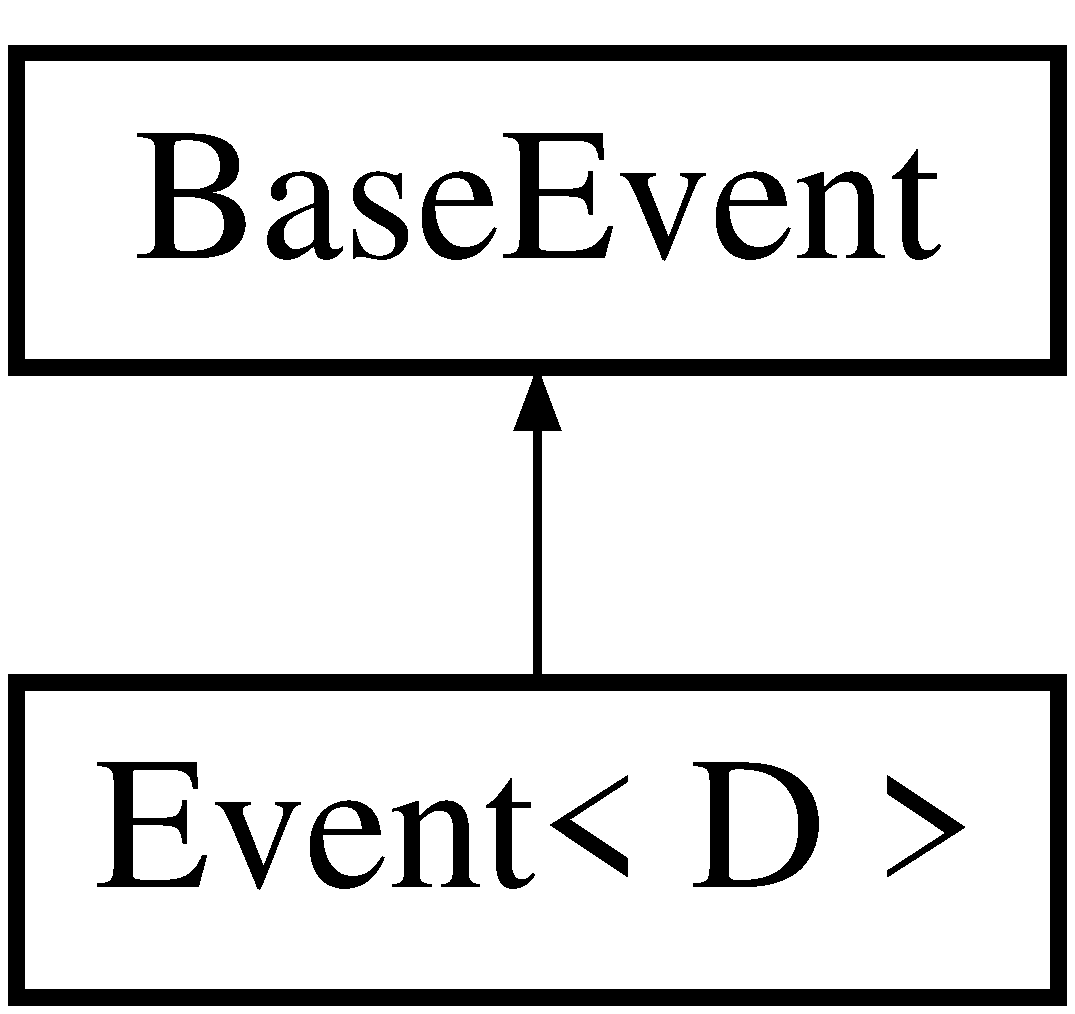
\includegraphics[height=2.000000cm]{classBaseEvent}
\end{center}
\end{figure}
\subsection*{Public Types}
\begin{DoxyCompactItemize}
\item 
\hypertarget{classBaseEvent_a2b68f24856d788f3abd3c3d812681343}{}enum {\bfseries Type} \{ {\bfseries none} = 0, 
{\bfseries swap\+Sessions}
 \}\label{classBaseEvent_a2b68f24856d788f3abd3c3d812681343}

\end{DoxyCompactItemize}
\subsection*{Public Member Functions}
\begin{DoxyCompactItemize}
\item 
\hypertarget{classBaseEvent_a41f97990ea1994b5e6feaa4a4f1a381e}{}{\bfseries Base\+Event} (const Type t=Type\+::none, const bool \hyperlink{classBaseEvent_a57cb919c14ba312f0a6c5e5bfdc52135}{interrupt}=false)\label{classBaseEvent_a41f97990ea1994b5e6feaa4a4f1a381e}

\end{DoxyCompactItemize}
\subsection*{Public Attributes}
\begin{DoxyCompactItemize}
\item 
\hypertarget{classBaseEvent_ae3a93c75173a29e77f9c51ffe7d49a47}{}const Type \hyperlink{classBaseEvent_ae3a93c75173a29e77f9c51ffe7d49a47}{type}\label{classBaseEvent_ae3a93c75173a29e77f9c51ffe7d49a47}

\begin{DoxyCompactList}\small\item\em event type \end{DoxyCompactList}\item 
\hypertarget{classBaseEvent_a57cb919c14ba312f0a6c5e5bfdc52135}{}const bool \hyperlink{classBaseEvent_a57cb919c14ba312f0a6c5e5bfdc52135}{interrupt}\label{classBaseEvent_a57cb919c14ba312f0a6c5e5bfdc52135}

\begin{DoxyCompactList}\small\item\em whether to interrupt drivers execution queue and jump to session loop in order to instantly parse \hyperlink{classEvent}{Event} \end{DoxyCompactList}\end{DoxyCompactItemize}


\subsection{Detailed Description}
The \hyperlink{classBaseEvent}{Base\+Event} class class providing events functionality designed for session management. 

Drivers can affect session flow by returning special Events. Base event doesn\textquotesingle{}t contain data, however drivers can create extended \hyperlink{classEvent}{Event} providing for example new session to be loaded.

\begin{DoxySeeAlso}{See also}
\hyperlink{classEvent}{Event} 
\end{DoxySeeAlso}


The documentation for this class was generated from the following file\+:\begin{DoxyCompactItemize}
\item 
include/Game\+Domain.\+h\end{DoxyCompactItemize}

\hypertarget{classChain}{}\section{Chain$<$ T\+Y\+P\+E $>$ Class Template Reference}
\label{classChain}\index{Chain$<$ T\+Y\+P\+E $>$@{Chain$<$ T\+Y\+P\+E $>$}}


\hyperlink{classChain}{Chain} class providing bi-\/directional-\/list like data organisation.  




{\ttfamily \#include $<$misc.\+h$>$}

\subsection*{Public Member Functions}
\begin{DoxyCompactItemize}
\item 
\hyperlink{classChain_a6e1b54f58b90218127399007e2be651a}{Chain} (T\+Y\+P\+E \hyperlink{classChain_aeb9b72f09201d5553bb04e25593dc7fa}{data})
\begin{DoxyCompactList}\small\item\em \hyperlink{classChain}{Chain} \hyperlink{classChain}{Chain} constructor. \end{DoxyCompactList}\item 
\hyperlink{classChain}{Chain} $\ast$ \hyperlink{classChain_a16411e8032aa4e0464d04d12f69577da}{next} ()
\begin{DoxyCompactList}\small\item\em next \end{DoxyCompactList}\item 
\hyperlink{classChain}{Chain} $\ast$ \hyperlink{classChain_a33dc961c1b75bdad1920680c56a7d52f}{prev} ()
\begin{DoxyCompactList}\small\item\em prev \end{DoxyCompactList}\item 
\hyperlink{classChain}{Chain} $\ast$ \hyperlink{classChain_a3251fcea46affc01835a565a0dcff0f6}{rewind} ()
\begin{DoxyCompactList}\small\item\em rewind \end{DoxyCompactList}\item 
\hyperlink{classChain}{Chain} $\ast$ \hyperlink{classChain_a83b9c24f7e9425bc4876f42833ff25d2}{rewind\+Forward} ()
\begin{DoxyCompactList}\small\item\em rewind\+Forward \end{DoxyCompactList}\item 
void \hyperlink{classChain_a8e044eca9ddb093211203a61c4aeb139}{insert\+After} (\hyperlink{classChain}{Chain} $\ast$c)
\begin{DoxyCompactList}\small\item\em insert\+After inserts given subchain after current element \end{DoxyCompactList}\item 
void \hyperlink{classChain_a47099e0a5193503c92458ffbb5ecb277}{insert\+Before} (\hyperlink{classChain}{Chain} $\ast$c)
\begin{DoxyCompactList}\small\item\em insert\+Before inserts given subchain before current elmenet \end{DoxyCompactList}\item 
void \hyperlink{classChain_adfec3f6f34ee095ffdb953418417ed63}{insert\+After} (T\+Y\+P\+E \hyperlink{classChain_aeb9b72f09201d5553bb04e25593dc7fa}{data})
\begin{DoxyCompactList}\small\item\em insert\+After inserts given data after current element \end{DoxyCompactList}\item 
void \hyperlink{classChain_a93b7323dd2f294dcfe07d6c67ec4619a}{insert\+Before} (T\+Y\+P\+E \hyperlink{classChain_aeb9b72f09201d5553bb04e25593dc7fa}{data})
\begin{DoxyCompactList}\small\item\em insert\+Before inserts given data before current elmenet \end{DoxyCompactList}\item 
\hypertarget{classChain_ad9ff2a0f87c43c3aa711c3ac5e3dc37a}{}void \hyperlink{classChain_ad9ff2a0f87c43c3aa711c3ac5e3dc37a}{pop} ()\label{classChain_ad9ff2a0f87c43c3aa711c3ac5e3dc37a}

\begin{DoxyCompactList}\small\item\em pop removes element from chain, creating new chain \end{DoxyCompactList}\item 
\hyperlink{classChain}{Chain}$<$ T\+Y\+P\+E $>$ $\ast$ \hyperlink{classChain_ace1c46fda105bc0cefe6337b793069de}{map} (void($\ast$f)(T\+Y\+P\+E \&))
\begin{DoxyCompactList}\small\item\em map replace content of all alements in array using provided function \end{DoxyCompactList}\item 
\hyperlink{classChain}{Chain}$<$ T\+Y\+P\+E $>$ $\ast$ \hyperlink{classChain_a5014320320b6044de28f27d7937165f3}{map} (T\+Y\+P\+E($\ast$f)(const T\+Y\+P\+E \&))
\begin{DoxyCompactList}\small\item\em map replace content of all alements in array using provided function \end{DoxyCompactList}\item 
\hyperlink{classChain}{Chain}$<$ T\+Y\+P\+E $>$ $\ast$ \hyperlink{classChain_ac21ec871573a170a704e6e06a9cac6ab}{each} (void($\ast$f)(const T\+Y\+P\+E \&))
\begin{DoxyCompactList}\small\item\em each calls provided function on all elements of array \end{DoxyCompactList}\item 
\hyperlink{classChain}{Chain}$<$ T\+Y\+P\+E $>$ $\ast$ \hyperlink{classChain_a95ad9170db946acf028ba2e98c349595}{selected} (void($\ast$f)(const T\+Y\+P\+E \&), bool($\ast$p)(const T\+Y\+P\+E \&))
\begin{DoxyCompactList}\small\item\em selected calls provided call function if acceptor function returns true \end{DoxyCompactList}\end{DoxyCompactItemize}
\subsection*{Public Attributes}
\begin{DoxyCompactItemize}
\item 
\hypertarget{classChain_aeb9b72f09201d5553bb04e25593dc7fa}{}T\+Y\+P\+E \hyperlink{classChain_aeb9b72f09201d5553bb04e25593dc7fa}{data}\label{classChain_aeb9b72f09201d5553bb04e25593dc7fa}

\begin{DoxyCompactList}\small\item\em data stored in each element \end{DoxyCompactList}\end{DoxyCompactItemize}


\subsection{Detailed Description}
\subsubsection*{template$<$class T\+Y\+P\+E$>$class Chain$<$ T\+Y\+P\+E $>$}

\hyperlink{classChain}{Chain} class providing bi-\/directional-\/list like data organisation. 

Each elemen has 2 neighbours. data access to any field is linear. Access to next/prev constant as well as adding/removing after/before current element. Due to its nature each element can be considered autonomous list thus each element popped from list using pop method becomes new list (in constant time/0 alloc) Template class gets stored data type as template param. 

\subsection{Constructor \& Destructor Documentation}
\hypertarget{classChain_a6e1b54f58b90218127399007e2be651a}{}\index{Chain@{Chain}!Chain@{Chain}}
\index{Chain@{Chain}!Chain@{Chain}}
\subsubsection[{Chain}]{\setlength{\rightskip}{0pt plus 5cm}template$<$class T\+Y\+P\+E$>$ {\bf Chain}$<$ T\+Y\+P\+E $>$\+::{\bf Chain} (
\begin{DoxyParamCaption}
\item[{T\+Y\+P\+E}]{data}
\end{DoxyParamCaption}
)\hspace{0.3cm}{\ttfamily [inline]}}\label{classChain_a6e1b54f58b90218127399007e2be651a}


\hyperlink{classChain}{Chain} \hyperlink{classChain}{Chain} constructor. 

Reqires data to be written into first 
\begin{DoxyParams}{Parameters}
{\em data} & data to be written as first element \\
\hline
\end{DoxyParams}


\subsection{Member Function Documentation}
\hypertarget{classChain_ac21ec871573a170a704e6e06a9cac6ab}{}\index{Chain@{Chain}!each@{each}}
\index{each@{each}!Chain@{Chain}}
\subsubsection[{each}]{\setlength{\rightskip}{0pt plus 5cm}template$<$class T\+Y\+P\+E$>$ {\bf Chain}$<$T\+Y\+P\+E$>$$\ast$ {\bf Chain}$<$ T\+Y\+P\+E $>$\+::each (
\begin{DoxyParamCaption}
\item[{void($\ast$)(const T\+Y\+P\+E \&)}]{f}
\end{DoxyParamCaption}
)\hspace{0.3cm}{\ttfamily [inline]}}\label{classChain_ac21ec871573a170a704e6e06a9cac6ab}


each calls provided function on all elements of array 


\begin{DoxyParams}{Parameters}
{\em f} & mapping function \\
\hline
\end{DoxyParams}
\begin{DoxyReturn}{Returns}

\end{DoxyReturn}
\hypertarget{classChain_a8e044eca9ddb093211203a61c4aeb139}{}\index{Chain@{Chain}!insert\+After@{insert\+After}}
\index{insert\+After@{insert\+After}!Chain@{Chain}}
\subsubsection[{insert\+After}]{\setlength{\rightskip}{0pt plus 5cm}template$<$class T\+Y\+P\+E$>$ void {\bf Chain}$<$ T\+Y\+P\+E $>$\+::insert\+After (
\begin{DoxyParamCaption}
\item[{{\bf Chain}$<$ T\+Y\+P\+E $>$ $\ast$}]{c}
\end{DoxyParamCaption}
)\hspace{0.3cm}{\ttfamily [inline]}}\label{classChain_a8e044eca9ddb093211203a61c4aeb139}


insert\+After inserts given subchain after current element 


\begin{DoxyParams}{Parameters}
{\em c} & subchain \\
\hline
\end{DoxyParams}
\hypertarget{classChain_adfec3f6f34ee095ffdb953418417ed63}{}\index{Chain@{Chain}!insert\+After@{insert\+After}}
\index{insert\+After@{insert\+After}!Chain@{Chain}}
\subsubsection[{insert\+After}]{\setlength{\rightskip}{0pt plus 5cm}template$<$class T\+Y\+P\+E$>$ void {\bf Chain}$<$ T\+Y\+P\+E $>$\+::insert\+After (
\begin{DoxyParamCaption}
\item[{T\+Y\+P\+E}]{data}
\end{DoxyParamCaption}
)\hspace{0.3cm}{\ttfamily [inline]}}\label{classChain_adfec3f6f34ee095ffdb953418417ed63}


insert\+After inserts given data after current element 


\begin{DoxyParams}{Parameters}
{\em data} & data \\
\hline
\end{DoxyParams}
\hypertarget{classChain_a47099e0a5193503c92458ffbb5ecb277}{}\index{Chain@{Chain}!insert\+Before@{insert\+Before}}
\index{insert\+Before@{insert\+Before}!Chain@{Chain}}
\subsubsection[{insert\+Before}]{\setlength{\rightskip}{0pt plus 5cm}template$<$class T\+Y\+P\+E$>$ void {\bf Chain}$<$ T\+Y\+P\+E $>$\+::insert\+Before (
\begin{DoxyParamCaption}
\item[{{\bf Chain}$<$ T\+Y\+P\+E $>$ $\ast$}]{c}
\end{DoxyParamCaption}
)\hspace{0.3cm}{\ttfamily [inline]}}\label{classChain_a47099e0a5193503c92458ffbb5ecb277}


insert\+Before inserts given subchain before current elmenet 


\begin{DoxyParams}{Parameters}
{\em c} & subchain \\
\hline
\end{DoxyParams}
\hypertarget{classChain_a93b7323dd2f294dcfe07d6c67ec4619a}{}\index{Chain@{Chain}!insert\+Before@{insert\+Before}}
\index{insert\+Before@{insert\+Before}!Chain@{Chain}}
\subsubsection[{insert\+Before}]{\setlength{\rightskip}{0pt plus 5cm}template$<$class T\+Y\+P\+E$>$ void {\bf Chain}$<$ T\+Y\+P\+E $>$\+::insert\+Before (
\begin{DoxyParamCaption}
\item[{T\+Y\+P\+E}]{data}
\end{DoxyParamCaption}
)\hspace{0.3cm}{\ttfamily [inline]}}\label{classChain_a93b7323dd2f294dcfe07d6c67ec4619a}


insert\+Before inserts given data before current elmenet 


\begin{DoxyParams}{Parameters}
{\em data} & data \\
\hline
\end{DoxyParams}
\hypertarget{classChain_ace1c46fda105bc0cefe6337b793069de}{}\index{Chain@{Chain}!map@{map}}
\index{map@{map}!Chain@{Chain}}
\subsubsection[{map}]{\setlength{\rightskip}{0pt plus 5cm}template$<$class T\+Y\+P\+E$>$ {\bf Chain}$<$T\+Y\+P\+E$>$$\ast$ {\bf Chain}$<$ T\+Y\+P\+E $>$\+::map (
\begin{DoxyParamCaption}
\item[{void($\ast$)(T\+Y\+P\+E \&)}]{f}
\end{DoxyParamCaption}
)\hspace{0.3cm}{\ttfamily [inline]}}\label{classChain_ace1c46fda105bc0cefe6337b793069de}


map replace content of all alements in array using provided function 


\begin{DoxyParams}{Parameters}
{\em f} & mapping function \\
\hline
\end{DoxyParams}
\begin{DoxyReturn}{Returns}
reference to \hyperlink{classArray}{Array} 
\end{DoxyReturn}
\hypertarget{classChain_a5014320320b6044de28f27d7937165f3}{}\index{Chain@{Chain}!map@{map}}
\index{map@{map}!Chain@{Chain}}
\subsubsection[{map}]{\setlength{\rightskip}{0pt plus 5cm}template$<$class T\+Y\+P\+E$>$ {\bf Chain}$<$T\+Y\+P\+E$>$$\ast$ {\bf Chain}$<$ T\+Y\+P\+E $>$\+::map (
\begin{DoxyParamCaption}
\item[{T\+Y\+P\+E($\ast$)(const T\+Y\+P\+E \&)}]{f}
\end{DoxyParamCaption}
)\hspace{0.3cm}{\ttfamily [inline]}}\label{classChain_a5014320320b6044de28f27d7937165f3}


map replace content of all alements in array using provided function 


\begin{DoxyParams}{Parameters}
{\em f} & mapping function \\
\hline
\end{DoxyParams}
\begin{DoxyReturn}{Returns}
reference to \hyperlink{classArray}{Array} 
\end{DoxyReturn}
\hypertarget{classChain_a16411e8032aa4e0464d04d12f69577da}{}\index{Chain@{Chain}!next@{next}}
\index{next@{next}!Chain@{Chain}}
\subsubsection[{next}]{\setlength{\rightskip}{0pt plus 5cm}template$<$class T\+Y\+P\+E$>$ {\bf Chain}$\ast$ {\bf Chain}$<$ T\+Y\+P\+E $>$\+::next (
\begin{DoxyParamCaption}
{}
\end{DoxyParamCaption}
)\hspace{0.3cm}{\ttfamily [inline]}}\label{classChain_a16411e8032aa4e0464d04d12f69577da}


next 

\begin{DoxyReturn}{Returns}
next chain elem 
\end{DoxyReturn}
\hypertarget{classChain_a33dc961c1b75bdad1920680c56a7d52f}{}\index{Chain@{Chain}!prev@{prev}}
\index{prev@{prev}!Chain@{Chain}}
\subsubsection[{prev}]{\setlength{\rightskip}{0pt plus 5cm}template$<$class T\+Y\+P\+E$>$ {\bf Chain}$\ast$ {\bf Chain}$<$ T\+Y\+P\+E $>$\+::prev (
\begin{DoxyParamCaption}
{}
\end{DoxyParamCaption}
)\hspace{0.3cm}{\ttfamily [inline]}}\label{classChain_a33dc961c1b75bdad1920680c56a7d52f}


prev 

\begin{DoxyReturn}{Returns}
prev chain elem 
\end{DoxyReturn}
\hypertarget{classChain_a3251fcea46affc01835a565a0dcff0f6}{}\index{Chain@{Chain}!rewind@{rewind}}
\index{rewind@{rewind}!Chain@{Chain}}
\subsubsection[{rewind}]{\setlength{\rightskip}{0pt plus 5cm}template$<$class T\+Y\+P\+E$>$ {\bf Chain}$\ast$ {\bf Chain}$<$ T\+Y\+P\+E $>$\+::rewind (
\begin{DoxyParamCaption}
{}
\end{DoxyParamCaption}
)\hspace{0.3cm}{\ttfamily [inline]}}\label{classChain_a3251fcea46affc01835a565a0dcff0f6}


rewind 

\begin{DoxyReturn}{Returns}
first chain elem 
\end{DoxyReturn}
\hypertarget{classChain_a83b9c24f7e9425bc4876f42833ff25d2}{}\index{Chain@{Chain}!rewind\+Forward@{rewind\+Forward}}
\index{rewind\+Forward@{rewind\+Forward}!Chain@{Chain}}
\subsubsection[{rewind\+Forward}]{\setlength{\rightskip}{0pt plus 5cm}template$<$class T\+Y\+P\+E$>$ {\bf Chain}$\ast$ {\bf Chain}$<$ T\+Y\+P\+E $>$\+::rewind\+Forward (
\begin{DoxyParamCaption}
{}
\end{DoxyParamCaption}
)\hspace{0.3cm}{\ttfamily [inline]}}\label{classChain_a83b9c24f7e9425bc4876f42833ff25d2}


rewind\+Forward 

\begin{DoxyReturn}{Returns}
last chain elem 
\end{DoxyReturn}
\hypertarget{classChain_a95ad9170db946acf028ba2e98c349595}{}\index{Chain@{Chain}!selected@{selected}}
\index{selected@{selected}!Chain@{Chain}}
\subsubsection[{selected}]{\setlength{\rightskip}{0pt plus 5cm}template$<$class T\+Y\+P\+E$>$ {\bf Chain}$<$T\+Y\+P\+E$>$$\ast$ {\bf Chain}$<$ T\+Y\+P\+E $>$\+::selected (
\begin{DoxyParamCaption}
\item[{void($\ast$)(const T\+Y\+P\+E \&)}]{f, }
\item[{bool($\ast$)(const T\+Y\+P\+E \&)}]{p}
\end{DoxyParamCaption}
)\hspace{0.3cm}{\ttfamily [inline]}}\label{classChain_a95ad9170db946acf028ba2e98c349595}


selected calls provided call function if acceptor function returns true 


\begin{DoxyParams}{Parameters}
{\em f} & call function \\
\hline
{\em acceptor} & function \\
\hline
\end{DoxyParams}
\begin{DoxyReturn}{Returns}

\end{DoxyReturn}


The documentation for this class was generated from the following file\+:\begin{DoxyCompactItemize}
\item 
include/misc.\+h\end{DoxyCompactItemize}

\hypertarget{classPhysicsEngine_1_1CollisionGrid}{}\section{Physics\+Engine\+:\+:Collision\+Grid Class Reference}
\label{classPhysicsEngine_1_1CollisionGrid}\index{Physics\+Engine\+::\+Collision\+Grid@{Physics\+Engine\+::\+Collision\+Grid}}


The \hyperlink{classPhysicsEngine_1_1CollisionGrid}{Collision\+Grid} class Class containing collision grid for optimization purpose.  




{\ttfamily \#include $<$physx.\+h$>$}

\subsection*{Classes}
\begin{DoxyCompactItemize}
\item 
struct \hyperlink{structPhysicsEngine_1_1CollisionGrid_1_1GridPool}{Grid\+Pool}
\begin{DoxyCompactList}\small\item\em $<$ grid pool entry \end{DoxyCompactList}\end{DoxyCompactItemize}
\subsection*{Public Member Functions}
\begin{DoxyCompactItemize}
\item 
\hyperlink{classPhysicsEngine_1_1CollisionGrid_a825fc5e0aaaf4eb9f663b957257ad804}{Collision\+Grid} (\hyperlink{classGameMap}{Game\+Map} \&map)
\begin{DoxyCompactList}\small\item\em \hyperlink{classPhysicsEngine_1_1CollisionGrid}{Collision\+Grid} Constructor. \end{DoxyCompactList}\item 
void \hyperlink{classPhysicsEngine_1_1CollisionGrid_aa82df2da2bcb18cd943e3f68c2099a42}{register\+Meta} (\hyperlink{classObjectPhysicsMeta}{Object\+Physics\+Meta} \&meta)
\begin{DoxyCompactList}\small\item\em register\+Meta register meta in collision grid \end{DoxyCompactList}\item 
void \hyperlink{classPhysicsEngine_1_1CollisionGrid_aef5fff9dd08c6adb65f4437536883da6}{erase\+Meta\+Records} (\hyperlink{classObjectPhysicsMeta}{Object\+Physics\+Meta} $\ast$meta)
\begin{DoxyCompactList}\small\item\em erase\+Meta\+Records remove meta from collision grid \end{DoxyCompactList}\end{DoxyCompactItemize}
\subsection*{Static Public Member Functions}
\begin{DoxyCompactItemize}
\item 
static \hyperlink{classVectorXY}{Vector\+X\+Y} \hyperlink{classPhysicsEngine_1_1CollisionGrid_adad4599413ced1499d2b8fb35d60034d}{get\+Object\+Bounds} (\hyperlink{classObjectPhysicsMeta}{Object\+Physics\+Meta} \&m)
\begin{DoxyCompactList}\small\item\em get\+Object\+Bounds returns bounding box occupied by object \end{DoxyCompactList}\end{DoxyCompactItemize}
\subsection*{Public Attributes}
\begin{DoxyCompactItemize}
\item 
\hypertarget{classPhysicsEngine_1_1CollisionGrid_a8453235376bf615693c1aa96f0f64744}{}const int \hyperlink{classPhysicsEngine_1_1CollisionGrid_a8453235376bf615693c1aa96f0f64744}{grid\+W}\label{classPhysicsEngine_1_1CollisionGrid_a8453235376bf615693c1aa96f0f64744}

\begin{DoxyCompactList}\small\item\em width of single sector \end{DoxyCompactList}\item 
\hypertarget{classPhysicsEngine_1_1CollisionGrid_ace91b9c4a8ff771dfb3bf27958a759f6}{}const int \hyperlink{classPhysicsEngine_1_1CollisionGrid_ace91b9c4a8ff771dfb3bf27958a759f6}{grid\+H}\label{classPhysicsEngine_1_1CollisionGrid_ace91b9c4a8ff771dfb3bf27958a759f6}

\begin{DoxyCompactList}\small\item\em height of single sector \end{DoxyCompactList}\item 
\hypertarget{classPhysicsEngine_1_1CollisionGrid_a603a2779e67a16deee6ffb44256ba44c}{}const int \hyperlink{classPhysicsEngine_1_1CollisionGrid_a603a2779e67a16deee6ffb44256ba44c}{grid\+C}\label{classPhysicsEngine_1_1CollisionGrid_a603a2779e67a16deee6ffb44256ba44c}

\begin{DoxyCompactList}\small\item\em number of columns in sectors grid \end{DoxyCompactList}\item 
\hypertarget{classPhysicsEngine_1_1CollisionGrid_ae430a085d671849fe2b0ae4ac15834d5}{}const int \hyperlink{classPhysicsEngine_1_1CollisionGrid_ae430a085d671849fe2b0ae4ac15834d5}{grid\+R}\label{classPhysicsEngine_1_1CollisionGrid_ae430a085d671849fe2b0ae4ac15834d5}

\begin{DoxyCompactList}\small\item\em number of rows in sectors grid \end{DoxyCompactList}\end{DoxyCompactItemize}
\subsection*{Friends}
\begin{DoxyCompactItemize}
\item 
\hypertarget{classPhysicsEngine_1_1CollisionGrid_a639ae8db08b48373cb96fa3728d3c447}{}class {\bfseries Physics\+Engine}\label{classPhysicsEngine_1_1CollisionGrid_a639ae8db08b48373cb96fa3728d3c447}

\end{DoxyCompactItemize}


\subsection{Detailed Description}
The \hyperlink{classPhysicsEngine_1_1CollisionGrid}{Collision\+Grid} class Class containing collision grid for optimization purpose. 

\subsection{Constructor \& Destructor Documentation}
\hypertarget{classPhysicsEngine_1_1CollisionGrid_a825fc5e0aaaf4eb9f663b957257ad804}{}\index{Physics\+Engine\+::\+Collision\+Grid@{Physics\+Engine\+::\+Collision\+Grid}!Collision\+Grid@{Collision\+Grid}}
\index{Collision\+Grid@{Collision\+Grid}!Physics\+Engine\+::\+Collision\+Grid@{Physics\+Engine\+::\+Collision\+Grid}}
\subsubsection[{Collision\+Grid}]{\setlength{\rightskip}{0pt plus 5cm}Physics\+Engine\+::\+Collision\+Grid\+::\+Collision\+Grid (
\begin{DoxyParamCaption}
\item[{{\bf Game\+Map} \&}]{map}
\end{DoxyParamCaption}
)}\label{classPhysicsEngine_1_1CollisionGrid_a825fc5e0aaaf4eb9f663b957257ad804}


\hyperlink{classPhysicsEngine_1_1CollisionGrid}{Collision\+Grid} Constructor. 


\begin{DoxyParams}{Parameters}
{\em map} & map to create grid for \\
\hline
\end{DoxyParams}


\subsection{Member Function Documentation}
\hypertarget{classPhysicsEngine_1_1CollisionGrid_aef5fff9dd08c6adb65f4437536883da6}{}\index{Physics\+Engine\+::\+Collision\+Grid@{Physics\+Engine\+::\+Collision\+Grid}!erase\+Meta\+Records@{erase\+Meta\+Records}}
\index{erase\+Meta\+Records@{erase\+Meta\+Records}!Physics\+Engine\+::\+Collision\+Grid@{Physics\+Engine\+::\+Collision\+Grid}}
\subsubsection[{erase\+Meta\+Records}]{\setlength{\rightskip}{0pt plus 5cm}void Physics\+Engine\+::\+Collision\+Grid\+::erase\+Meta\+Records (
\begin{DoxyParamCaption}
\item[{{\bf Object\+Physics\+Meta} $\ast$}]{meta}
\end{DoxyParamCaption}
)}\label{classPhysicsEngine_1_1CollisionGrid_aef5fff9dd08c6adb65f4437536883da6}


erase\+Meta\+Records remove meta from collision grid 


\begin{DoxyParams}{Parameters}
{\em meta} & meta to be removed \\
\hline
\end{DoxyParams}
\hypertarget{classPhysicsEngine_1_1CollisionGrid_adad4599413ced1499d2b8fb35d60034d}{}\index{Physics\+Engine\+::\+Collision\+Grid@{Physics\+Engine\+::\+Collision\+Grid}!get\+Object\+Bounds@{get\+Object\+Bounds}}
\index{get\+Object\+Bounds@{get\+Object\+Bounds}!Physics\+Engine\+::\+Collision\+Grid@{Physics\+Engine\+::\+Collision\+Grid}}
\subsubsection[{get\+Object\+Bounds}]{\setlength{\rightskip}{0pt plus 5cm}{\bf Vector\+X\+Y} Physics\+Engine\+::\+Collision\+Grid\+::get\+Object\+Bounds (
\begin{DoxyParamCaption}
\item[{{\bf Object\+Physics\+Meta} \&}]{m}
\end{DoxyParamCaption}
)\hspace{0.3cm}{\ttfamily [static]}}\label{classPhysicsEngine_1_1CollisionGrid_adad4599413ced1499d2b8fb35d60034d}


get\+Object\+Bounds returns bounding box occupied by object 


\begin{DoxyParams}{Parameters}
{\em m} & meta of requested object \\
\hline
\end{DoxyParams}
\begin{DoxyReturn}{Returns}
pair top left corner \+: bottom right corner 
\end{DoxyReturn}
\hypertarget{classPhysicsEngine_1_1CollisionGrid_aa82df2da2bcb18cd943e3f68c2099a42}{}\index{Physics\+Engine\+::\+Collision\+Grid@{Physics\+Engine\+::\+Collision\+Grid}!register\+Meta@{register\+Meta}}
\index{register\+Meta@{register\+Meta}!Physics\+Engine\+::\+Collision\+Grid@{Physics\+Engine\+::\+Collision\+Grid}}
\subsubsection[{register\+Meta}]{\setlength{\rightskip}{0pt plus 5cm}void Physics\+Engine\+::\+Collision\+Grid\+::register\+Meta (
\begin{DoxyParamCaption}
\item[{{\bf Object\+Physics\+Meta} \&}]{meta}
\end{DoxyParamCaption}
)}\label{classPhysicsEngine_1_1CollisionGrid_aa82df2da2bcb18cd943e3f68c2099a42}


register\+Meta register meta in collision grid 


\begin{DoxyParams}{Parameters}
{\em meta} & meta to be registered \\
\hline
\end{DoxyParams}


The documentation for this class was generated from the following files\+:\begin{DoxyCompactItemize}
\item 
include/physx.\+h\item 
src/physx.\+cpp\end{DoxyCompactItemize}

\hypertarget{structPhysicsEngine_1_1CREnt}{}\section{Physics\+Engine\+:\+:C\+R\+Ent Struct Reference}
\label{structPhysicsEngine_1_1CREnt}\index{Physics\+Engine\+::\+C\+R\+Ent@{Physics\+Engine\+::\+C\+R\+Ent}}
\subsection*{Public Attributes}
\begin{DoxyCompactItemize}
\item 
\hypertarget{structPhysicsEngine_1_1CREnt_aec2696b42ec2eb20313266df7245949d}{}\hyperlink{classObjectPhysicsMeta}{Object\+Physics\+Meta} $\ast$ \hyperlink{structPhysicsEngine_1_1CREnt_aec2696b42ec2eb20313266df7245949d}{A}\label{structPhysicsEngine_1_1CREnt_aec2696b42ec2eb20313266df7245949d}

\begin{DoxyCompactList}\small\item\em $<$ collision registry entry struct \end{DoxyCompactList}\item 
\hypertarget{structPhysicsEngine_1_1CREnt_a489aa40e4a140f2be01085b09e8e41fb}{}\hyperlink{classObjectPhysicsMeta}{Object\+Physics\+Meta} $\ast$ {\bfseries B}\label{structPhysicsEngine_1_1CREnt_a489aa40e4a140f2be01085b09e8e41fb}

\end{DoxyCompactItemize}


The documentation for this struct was generated from the following file\+:\begin{DoxyCompactItemize}
\item 
include/physx.\+h\end{DoxyCompactItemize}

\hypertarget{classDecal}{}\section{Decal Class Reference}
\label{classDecal}\index{Decal@{Decal}}


The \hyperlink{classDecal}{Decal} class renderable \hyperlink{classDecal}{Decal} for Render Engine.  




{\ttfamily \#include $<$object.\+h$>$}

Inheritance diagram for Decal\+:\begin{figure}[H]
\begin{center}
\leavevmode
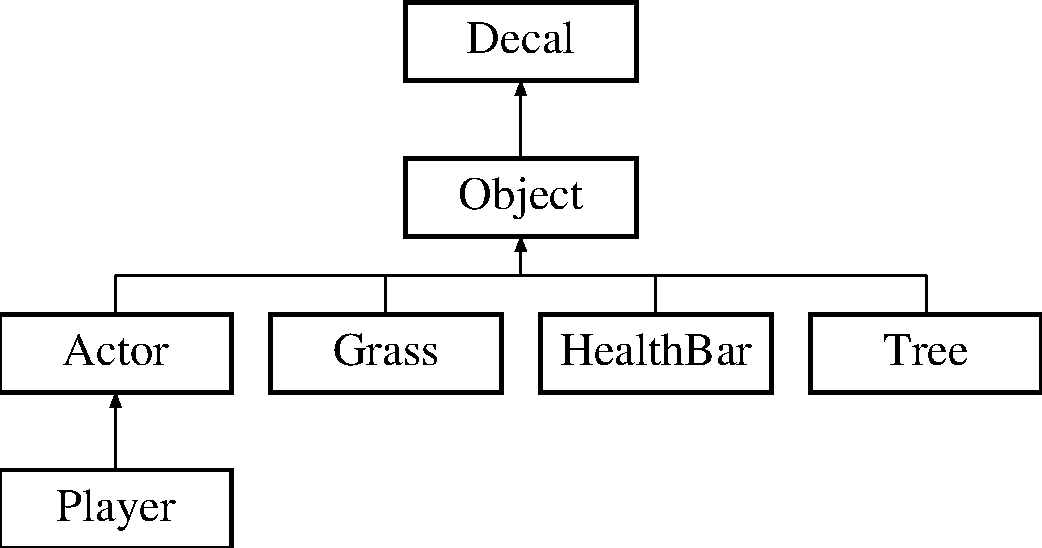
\includegraphics[height=4.000000cm]{classDecal}
\end{center}
\end{figure}
\subsection*{Public Member Functions}
\begin{DoxyCompactItemize}
\item 
\hyperlink{classDecal_aea7ec36355a8c52f05bfcdeb2a7afd39}{Decal} (const char $\ast$file\+Path=Decal\+::void\+Texture\+Path, \hyperlink{classPointXY}{Point\+X\+Y} \hyperlink{classDecal_a9db398b189cffe1f8770f8bce5b8af71}{offset}=\hyperlink{classPointXY}{Point\+X\+Y}(0, 0))
\begin{DoxyCompactList}\small\item\em \hyperlink{classDecal}{Decal} basic constructor of \hyperlink{classDecal}{Decal}. \end{DoxyCompactList}\end{DoxyCompactItemize}
\subsection*{Public Attributes}
\begin{DoxyCompactItemize}
\item 
\hypertarget{classDecal_a3705e76536e078915d8ebfb6a16434fe}{}const sf\+::\+Texture $\ast$ \hyperlink{classDecal_a3705e76536e078915d8ebfb6a16434fe}{texture}\label{classDecal_a3705e76536e078915d8ebfb6a16434fe}

\begin{DoxyCompactList}\small\item\em texture contained by \hyperlink{classDecal}{Decal} \end{DoxyCompactList}\item 
\hypertarget{classDecal_a9db398b189cffe1f8770f8bce5b8af71}{}const \hyperlink{classPointXY}{Point\+X\+Y} \hyperlink{classDecal_a9db398b189cffe1f8770f8bce5b8af71}{offset}\label{classDecal_a9db398b189cffe1f8770f8bce5b8af71}

\begin{DoxyCompactList}\small\item\em offset of texture to be applied when rendering \end{DoxyCompactList}\end{DoxyCompactItemize}
\subsection*{Static Public Attributes}
\begin{DoxyCompactItemize}
\item 
\hypertarget{classDecal_ae0aef82d67996f23e2ea73795445188e}{}static constexpr char $\ast$ {\bfseries void\+Texture\+Path} =(char$\ast$)\char`\"{}misc/void.\+png\char`\"{}\label{classDecal_ae0aef82d67996f23e2ea73795445188e}

\end{DoxyCompactItemize}


\subsection{Detailed Description}
The \hyperlink{classDecal}{Decal} class renderable \hyperlink{classDecal}{Decal} for Render Engine. 

\subsection{Constructor \& Destructor Documentation}
\hypertarget{classDecal_aea7ec36355a8c52f05bfcdeb2a7afd39}{}\index{Decal@{Decal}!Decal@{Decal}}
\index{Decal@{Decal}!Decal@{Decal}}
\subsubsection[{Decal}]{\setlength{\rightskip}{0pt plus 5cm}Decal\+::\+Decal (
\begin{DoxyParamCaption}
\item[{const char $\ast$}]{file\+Path = {\ttfamily Decal\+:\+:voidTexturePath}, }
\item[{{\bf Point\+X\+Y}}]{offset = {\ttfamily {\bf Point\+X\+Y}(0,0)}}
\end{DoxyParamCaption}
)}\label{classDecal_aea7ec36355a8c52f05bfcdeb2a7afd39}


\hyperlink{classDecal}{Decal} basic constructor of \hyperlink{classDecal}{Decal}. 


\begin{DoxyParams}{Parameters}
{\em file\+Path} & path to file to be used as texture \\
\hline
{\em offset} & (optional) offset of texture \\
\hline
\end{DoxyParams}


The documentation for this class was generated from the following files\+:\begin{DoxyCompactItemize}
\item 
include/object.\+h\item 
src/object.\+cpp\end{DoxyCompactItemize}

\hypertarget{classEngineStart}{}\section{Engine\+Start Class Reference}
\label{classEngineStart}\index{Engine\+Start@{Engine\+Start}}


The \hyperlink{classEngineStart}{Engine\+Start} class is using as a tool which will control current session and will change session when user press return.  




{\ttfamily \#include $<$Engine\+Start.\+h$>$}

Inheritance diagram for Engine\+Start\+:\begin{figure}[H]
\begin{center}
\leavevmode
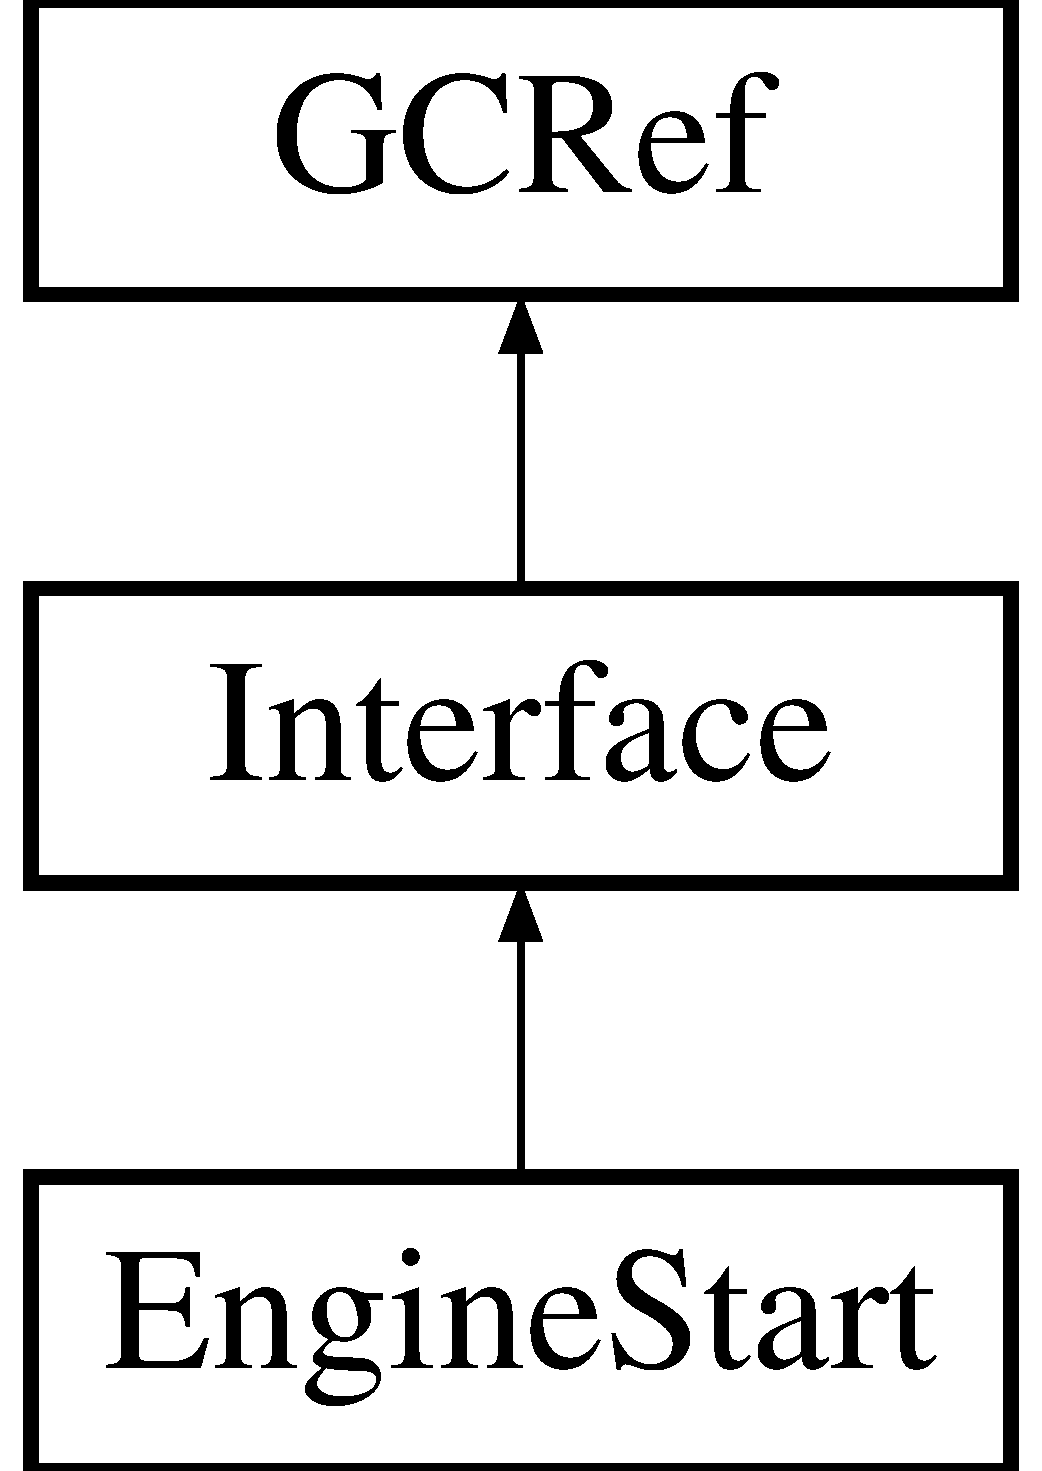
\includegraphics[height=3.000000cm]{classEngineStart}
\end{center}
\end{figure}
\subsection*{Public Member Functions}
\begin{DoxyCompactItemize}
\item 
\hypertarget{classEngineStart_aa40d0a5b9d72a3ce33a8f8fa99656b08}{}{\bfseries Engine\+Start} (\hyperlink{classRenderEngine}{Render\+Engine} \&r\+E)\label{classEngineStart_aa40d0a5b9d72a3ce33a8f8fa99656b08}

\item 
\hyperlink{classBaseEvent}{Base\+Event} \& \hyperlink{classEngineStart_a9caa9db3213371e5a77f1b09576a04fa}{run} (\hyperlink{classGameSession}{Game\+Session} \&session)
\begin{DoxyCompactList}\small\item\em Basic methods which give us a opportunity to control a session. \end{DoxyCompactList}\item 
\hypertarget{classEngineStart_aa69bfc21de9586ba2058aa07d9790b02}{}void \hyperlink{classEngineStart_aa69bfc21de9586ba2058aa07d9790b02}{set\+Is\+Object\+Added} (bool C=true)\label{classEngineStart_aa69bfc21de9586ba2058aa07d9790b02}

\begin{DoxyCompactList}\small\item\em Change a class variable Is\+Object\+Added. \end{DoxyCompactList}\end{DoxyCompactItemize}


\subsection{Detailed Description}
The \hyperlink{classEngineStart}{Engine\+Start} class is using as a tool which will control current session and will change session when user press return. 

\begin{DoxySeeAlso}{See also}
\hyperlink{classInterface}{Interface} 
\end{DoxySeeAlso}


\subsection{Member Function Documentation}
\hypertarget{classEngineStart_a9caa9db3213371e5a77f1b09576a04fa}{}\index{Engine\+Start@{Engine\+Start}!run@{run}}
\index{run@{run}!Engine\+Start@{Engine\+Start}}
\subsubsection[{run}]{\setlength{\rightskip}{0pt plus 5cm}{\bf Base\+Event} \& Engine\+Start\+::run (
\begin{DoxyParamCaption}
\item[{{\bf Game\+Session} \&}]{session}
\end{DoxyParamCaption}
)\hspace{0.3cm}{\ttfamily [virtual]}}\label{classEngineStart_a9caa9db3213371e5a77f1b09576a04fa}


Basic methods which give us a opportunity to control a session. 

D\+O\+D\+A\+J\+E K\+L\+O\+C\+E\+K K\+T\+O\+R\+Y W R\+U\+N Z\+W\+R\+A\+C\+A swap\+S\+E\+S\+S\+I\+O\+N\+S 

Implements \hyperlink{classInterface_addff25eb2adf4221c2be4895597b49c1}{Interface}.



The documentation for this class was generated from the following files\+:\begin{DoxyCompactItemize}
\item 
drivers/include/Engine\+Start.\+h\item 
drivers/src/Engine\+Start.\+cpp\end{DoxyCompactItemize}

\hypertarget{classEvent}{}\section{Event$<$ D $>$ Class Template Reference}
\label{classEvent}\index{Event$<$ D $>$@{Event$<$ D $>$}}


The \hyperlink{classEvent}{Event} class extension to \hyperlink{classBaseEvent}{Base\+Event} class allowing drivers to pass custom data in event.  




{\ttfamily \#include $<$Game\+Domain.\+h$>$}

Inheritance diagram for Event$<$ D $>$\+:\begin{figure}[H]
\begin{center}
\leavevmode
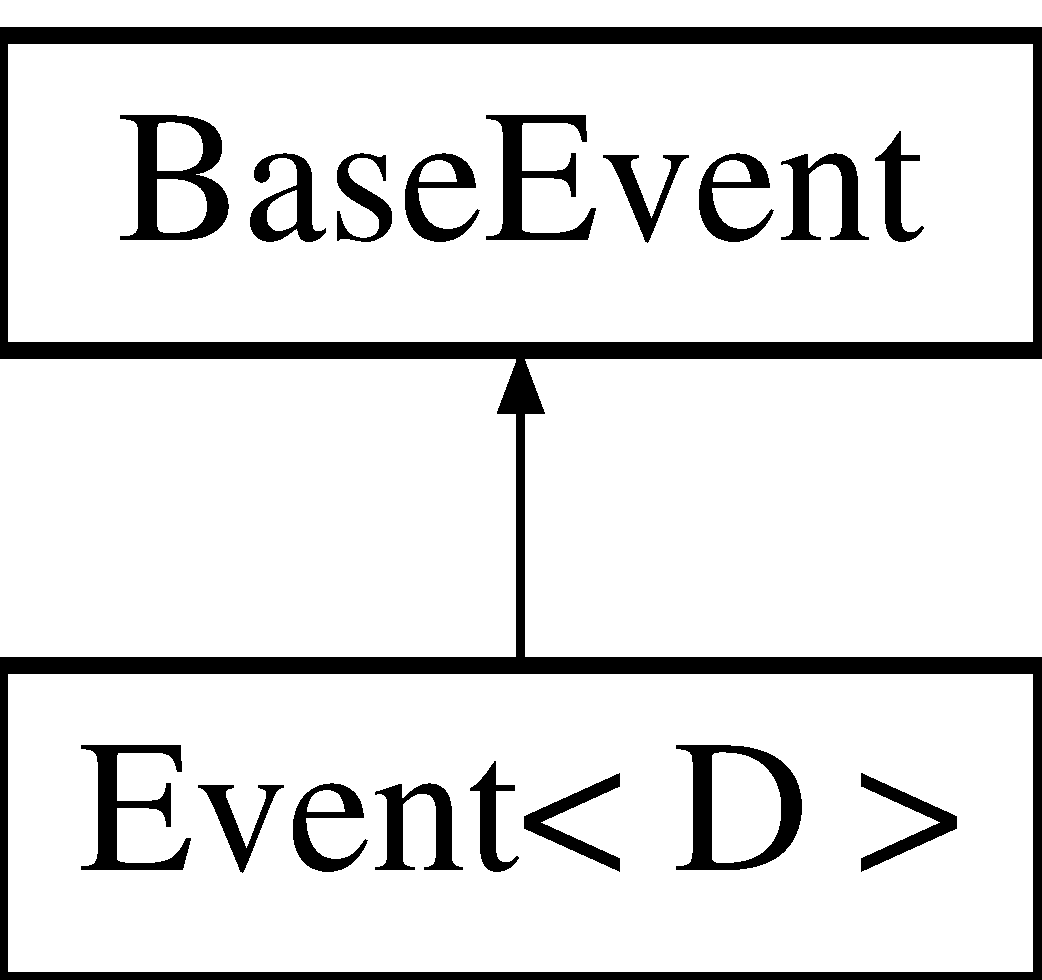
\includegraphics[height=2.000000cm]{classEvent}
\end{center}
\end{figure}
\subsection*{Public Member Functions}
\begin{DoxyCompactItemize}
\item 
\hypertarget{classEvent_a9f4c099332063f31a73277fb3dc74e30}{}{\bfseries Event} (const D \hyperlink{classEvent_a1e5208ad8d92b27baa16087db4cbe921}{data}, const Type t=Type\+::none, const bool \hyperlink{classBaseEvent_a57cb919c14ba312f0a6c5e5bfdc52135}{interrupt}=false)\label{classEvent_a9f4c099332063f31a73277fb3dc74e30}

\end{DoxyCompactItemize}
\subsection*{Public Attributes}
\begin{DoxyCompactItemize}
\item 
\hypertarget{classEvent_a1e5208ad8d92b27baa16087db4cbe921}{}const D \hyperlink{classEvent_a1e5208ad8d92b27baa16087db4cbe921}{data}\label{classEvent_a1e5208ad8d92b27baa16087db4cbe921}

\begin{DoxyCompactList}\small\item\em custom data \end{DoxyCompactList}\end{DoxyCompactItemize}
\subsection*{Additional Inherited Members}


\subsection{Detailed Description}
\subsubsection*{template$<$typename D$>$class Event$<$ D $>$}

The \hyperlink{classEvent}{Event} class extension to \hyperlink{classBaseEvent}{Base\+Event} class allowing drivers to pass custom data in event. 

\begin{DoxySeeAlso}{See also}
\hyperlink{classBaseEvent}{Base\+Event} 
\end{DoxySeeAlso}


The documentation for this class was generated from the following file\+:\begin{DoxyCompactItemize}
\item 
include/Game\+Domain.\+h\end{DoxyCompactItemize}

\hypertarget{classGameDomain}{}\section{Game\+Domain Class Reference}
\label{classGameDomain}\index{Game\+Domain@{Game\+Domain}}


The \hyperlink{classGameDomain}{Game\+Domain} class Game domain manager class, providing game domain code layer for game logic.  




{\ttfamily \#include $<$Game\+Domain.\+h$>$}

\subsection*{Public Member Functions}
\begin{DoxyCompactItemize}
\item 
void \hyperlink{classGameDomain_af4426ea0c66b01e5c573becf180e7fb3}{add} (\hyperlink{classInterface}{Interface} \&interface)
\begin{DoxyCompactList}\small\item\em add add new driver to execution queue of this manager \end{DoxyCompactList}\item 
void \hyperlink{classGameDomain_a77944f3e82e8f492c523586dd1ce0674}{remove} (\hyperlink{classInterface}{Interface} $\ast$interface)
\begin{DoxyCompactList}\small\item\em remove remove driver from manager \end{DoxyCompactList}\item 
void \hyperlink{classGameDomain_a8326ffd8483813cd617c13e6d8e0dbfc}{bind\+Session} (\hyperlink{classGameSession}{Game\+Session} \&s)
\begin{DoxyCompactList}\small\item\em bind\+Session bind session to this manager. \end{DoxyCompactList}\item 
\hyperlink{classChain}{Chain}$<$ \hyperlink{classBaseEvent}{Base\+Event} \& $>$ $\ast$ \hyperlink{classGameDomain_a9d8996f5abf6019a7a396c1854a3b8eb}{reload} ()
\begin{DoxyCompactList}\small\item\em reload reload drivers queue \end{DoxyCompactList}\end{DoxyCompactItemize}


\subsection{Detailed Description}
The \hyperlink{classGameDomain}{Game\+Domain} class Game domain manager class, providing game domain code layer for game logic. 

Game is created using multiple drivers, handling various tasks. 

\subsection{Member Function Documentation}
\hypertarget{classGameDomain_af4426ea0c66b01e5c573becf180e7fb3}{}\index{Game\+Domain@{Game\+Domain}!add@{add}}
\index{add@{add}!Game\+Domain@{Game\+Domain}}
\subsubsection[{add}]{\setlength{\rightskip}{0pt plus 5cm}void Game\+Domain\+::add (
\begin{DoxyParamCaption}
\item[{{\bf Interface} \&}]{interface}
\end{DoxyParamCaption}
)}\label{classGameDomain_af4426ea0c66b01e5c573becf180e7fb3}


add add new driver to execution queue of this manager 


\begin{DoxyParams}{Parameters}
{\em interface} & interface to be added \\
\hline
\end{DoxyParams}
\hypertarget{classGameDomain_a8326ffd8483813cd617c13e6d8e0dbfc}{}\index{Game\+Domain@{Game\+Domain}!bind\+Session@{bind\+Session}}
\index{bind\+Session@{bind\+Session}!Game\+Domain@{Game\+Domain}}
\subsubsection[{bind\+Session}]{\setlength{\rightskip}{0pt plus 5cm}void Game\+Domain\+::bind\+Session (
\begin{DoxyParamCaption}
\item[{{\bf Game\+Session} \&}]{s}
\end{DoxyParamCaption}
)\hspace{0.3cm}{\ttfamily [inline]}}\label{classGameDomain_a8326ffd8483813cd617c13e6d8e0dbfc}


bind\+Session bind session to this manager. 

T\+H\+I\+S I\+S R\+E\+Q\+U\+I\+R\+E\+D. Each manager H\+A\+S T\+O have some session bound to it. 
\begin{DoxyParams}{Parameters}
{\em s} & session to be bound \\
\hline
\end{DoxyParams}
\hypertarget{classGameDomain_a9d8996f5abf6019a7a396c1854a3b8eb}{}\index{Game\+Domain@{Game\+Domain}!reload@{reload}}
\index{reload@{reload}!Game\+Domain@{Game\+Domain}}
\subsubsection[{reload}]{\setlength{\rightskip}{0pt plus 5cm}{\bf Chain}$<$ {\bf Base\+Event} \& $>$ $\ast$ Game\+Domain\+::reload (
\begin{DoxyParamCaption}
{}
\end{DoxyParamCaption}
)}\label{classGameDomain_a9d8996f5abf6019a7a396c1854a3b8eb}


reload reload drivers queue 

\begin{DoxyReturn}{Returns}

\end{DoxyReturn}
\hypertarget{classGameDomain_a77944f3e82e8f492c523586dd1ce0674}{}\index{Game\+Domain@{Game\+Domain}!remove@{remove}}
\index{remove@{remove}!Game\+Domain@{Game\+Domain}}
\subsubsection[{remove}]{\setlength{\rightskip}{0pt plus 5cm}void Game\+Domain\+::remove (
\begin{DoxyParamCaption}
\item[{{\bf Interface} $\ast$}]{interface}
\end{DoxyParamCaption}
)}\label{classGameDomain_a77944f3e82e8f492c523586dd1ce0674}


remove remove driver from manager 


\begin{DoxyParams}{Parameters}
{\em interface} & to be removed \\
\hline
\end{DoxyParams}


The documentation for this class was generated from the following files\+:\begin{DoxyCompactItemize}
\item 
include/Game\+Domain.\+h\item 
src/Game\+Domain.\+cpp\end{DoxyCompactItemize}

\hypertarget{classGameEngine}{}\section{Game\+Engine Class Reference}
\label{classGameEngine}\index{Game\+Engine@{Game\+Engine}}


The \hyperlink{classGameEngine}{Game\+Engine} class main game engine class.  




{\ttfamily \#include $<$engine.\+h$>$}

\subsection*{Public Member Functions}
\begin{DoxyCompactItemize}
\item 
void \hyperlink{classGameEngine_a6aa48e7ec713a0570e7a699b0935e337}{start} (bool \&interrupt\+Trigger)
\begin{DoxyCompactList}\small\item\em start start new game \end{DoxyCompactList}\item 
void \hyperlink{classGameEngine_a5411662bf860c553a85c470024a16265}{purge\+Session} (\hyperlink{classGameSession}{Game\+Session} $\ast$session)
\begin{DoxyCompactList}\small\item\em purge\+Session delete specified session (sned it to the mooooon) \end{DoxyCompactList}\end{DoxyCompactItemize}


\subsection{Detailed Description}
The \hyperlink{classGameEngine}{Game\+Engine} class main game engine class. 

\subsection{Member Function Documentation}
\hypertarget{classGameEngine_a5411662bf860c553a85c470024a16265}{}\index{Game\+Engine@{Game\+Engine}!purge\+Session@{purge\+Session}}
\index{purge\+Session@{purge\+Session}!Game\+Engine@{Game\+Engine}}
\subsubsection[{purge\+Session}]{\setlength{\rightskip}{0pt plus 5cm}void Game\+Engine\+::purge\+Session (
\begin{DoxyParamCaption}
\item[{{\bf Game\+Session} $\ast$}]{session}
\end{DoxyParamCaption}
)}\label{classGameEngine_a5411662bf860c553a85c470024a16265}


purge\+Session delete specified session (sned it to the mooooon) 


\begin{DoxyParams}{Parameters}
{\em session} & session to be deleted \\
\hline
\end{DoxyParams}
\hypertarget{classGameEngine_a6aa48e7ec713a0570e7a699b0935e337}{}\index{Game\+Engine@{Game\+Engine}!start@{start}}
\index{start@{start}!Game\+Engine@{Game\+Engine}}
\subsubsection[{start}]{\setlength{\rightskip}{0pt plus 5cm}void Game\+Engine\+::start (
\begin{DoxyParamCaption}
\item[{bool \&}]{interrupt\+Trigger}
\end{DoxyParamCaption}
)}\label{classGameEngine_a6aa48e7ec713a0570e7a699b0935e337}


start start new game 


\begin{DoxyParams}{Parameters}
{\em interrupt\+Trigger} & reference to bool triggering extraordinary execution interruption \\
\hline
\end{DoxyParams}


The documentation for this class was generated from the following files\+:\begin{DoxyCompactItemize}
\item 
include/engine.\+h\item 
src/engine.\+cpp\end{DoxyCompactItemize}

\hypertarget{classGameMap}{}\section{Game\+Map Class Reference}
\label{classGameMap}\index{Game\+Map@{Game\+Map}}


The \hyperlink{classGameMap}{Game\+Map} class Map class.  




{\ttfamily \#include $<$map.\+h$>$}

\subsection*{Public Member Functions}
\begin{DoxyCompactItemize}
\item 
\hyperlink{classGameMap_a094aba2348a0265746326b6c1d1864f2}{Game\+Map} (int \hyperlink{classGameMap_ae9f5144c59e2749104bf8a47f1fd8eb3}{width}=64, int heigth=48)
\begin{DoxyCompactList}\small\item\em \hyperlink{classGameMap}{Game\+Map} Map constructor. \end{DoxyCompactList}\item 
int \hyperlink{classGameMap_a0cfbeb2c0b6a270fc5fa1bcd140743cc}{get\+Index} (const \hyperlink{classObjectMapMeta}{Object\+Map\+Meta} $\ast$meta) const 
\begin{DoxyCompactList}\small\item\em get\+Index searches for specified meta in map objects list and returns index \end{DoxyCompactList}\item 
\hyperlink{classObjectMapMeta}{Object\+Map\+Meta} \& \hyperlink{classGameMap_a3b7cf2fcc2a675b2a66ab304f5d115ad}{get\+Meta} (int index) const 
\begin{DoxyCompactList}\small\item\em get\+Meta returns object meta from given position in objects list \end{DoxyCompactList}\item 
void \hyperlink{classGameMap_a1445fd0bb55e7e4ad9fe3cc780306e2d}{add\+Object} (\hyperlink{classObject}{Object} \&obj, \hyperlink{classPointXY}{Point\+X\+Y} pos=\hyperlink{classPointXY}{Point\+X\+Y}(0, 0))
\begin{DoxyCompactList}\small\item\em add\+Object Places object on map \end{DoxyCompactList}\item 
void \hyperlink{classGameMap_a7ba7b031db20572304e9d1af751ead53}{add\+Object} (\hyperlink{classObjectMapMeta}{Object\+Map\+Meta} \&meta)
\begin{DoxyCompactList}\small\item\em add\+Object Places meta on map \end{DoxyCompactList}\item 
\hyperlink{classObjectMapMeta}{Object\+Map\+Meta} \& \hyperlink{classGameMap_a48e62c1eccddabdf34b01c23e17ad07a}{pop\+Object} (\hyperlink{classObjectMapMeta}{Object\+Map\+Meta} $\ast$meta)
\begin{DoxyCompactList}\small\item\em pop\+Object removes meta from map (specified by meta) \end{DoxyCompactList}\item 
\hyperlink{classObjectMapMeta}{Object\+Map\+Meta} \& \hyperlink{classGameMap_aae79574a7e15275ad8bff7aa1d109f32}{pop\+Object} (int index)
\begin{DoxyCompactList}\small\item\em pop\+Object removes meta from map (specified by index) \end{DoxyCompactList}\item 
void \hyperlink{classGameMap_ac0bec0f4d4de18a568b952b525e37ce4}{delete\+Object} (\hyperlink{classObjectMapMeta}{Object\+Map\+Meta} $\ast$meta)
\begin{DoxyCompactList}\small\item\em delete\+Object deletes meta (specified by meta) \end{DoxyCompactList}\item 
void \hyperlink{classGameMap_a0177ce70320072c9eaaf0a14f559ca8a}{delete\+Object} (int index)
\begin{DoxyCompactList}\small\item\em delete\+Object deletes meta (specified by index) \end{DoxyCompactList}\item 
\hypertarget{classGameMap_a27fe5bad0af175eb8bf65254262b96cf}{}void \hyperlink{classGameMap_a27fe5bad0af175eb8bf65254262b96cf}{clear} ()\label{classGameMap_a27fe5bad0af175eb8bf65254262b96cf}

\begin{DoxyCompactList}\small\item\em clear Clears map from all objects \end{DoxyCompactList}\item 
\hyperlink{classObjectMapMeta}{Object\+Map\+Meta} \& \hyperlink{classGameMap_af4ce25ca7060ef9a175f75075364d9c0}{operator\mbox{[}$\,$\mbox{]}} (const int \&index) const 
\begin{DoxyCompactList}\small\item\em operator \mbox{[}\mbox{]} table operator for map. \end{DoxyCompactList}\item 
\hypertarget{classGameMap_ac1001868696aa67e05070149376ea7d9}{}int {\bfseries operator\mbox{[}$\,$\mbox{]}} (const \hyperlink{classObjectMapMeta}{Object\+Map\+Meta} \&m) const \label{classGameMap_ac1001868696aa67e05070149376ea7d9}

\item 
\hypertarget{classGameMap_a0352e28044e91dd51dfa0d70a10e71ad}{}int {\bfseries length} ()\label{classGameMap_a0352e28044e91dd51dfa0d70a10e71ad}

\end{DoxyCompactItemize}
\subsection*{Public Attributes}
\begin{DoxyCompactItemize}
\item 
\hypertarget{classGameMap_ae9f5144c59e2749104bf8a47f1fd8eb3}{}const int \hyperlink{classGameMap_ae9f5144c59e2749104bf8a47f1fd8eb3}{width}\label{classGameMap_ae9f5144c59e2749104bf8a47f1fd8eb3}

\begin{DoxyCompactList}\small\item\em map width \end{DoxyCompactList}\item 
\hypertarget{classGameMap_a7d35b81d7d8e64820bfd2c9e5d8e708d}{}const int \hyperlink{classGameMap_a7d35b81d7d8e64820bfd2c9e5d8e708d}{height}\label{classGameMap_a7d35b81d7d8e64820bfd2c9e5d8e708d}

\begin{DoxyCompactList}\small\item\em map height \end{DoxyCompactList}\end{DoxyCompactItemize}


\subsection{Detailed Description}
The \hyperlink{classGameMap}{Game\+Map} class Map class. 

Contains objects.

\begin{DoxySeeAlso}{See also}
\hyperlink{classObjectMapMeta}{Object\+Map\+Meta} 

\hyperlink{classPhysicsEngine}{Physics\+Engine} 
\end{DoxySeeAlso}


\subsection{Constructor \& Destructor Documentation}
\hypertarget{classGameMap_a094aba2348a0265746326b6c1d1864f2}{}\index{Game\+Map@{Game\+Map}!Game\+Map@{Game\+Map}}
\index{Game\+Map@{Game\+Map}!Game\+Map@{Game\+Map}}
\subsubsection[{Game\+Map}]{\setlength{\rightskip}{0pt plus 5cm}Game\+Map\+::\+Game\+Map (
\begin{DoxyParamCaption}
\item[{int}]{width = {\ttfamily 64}, }
\item[{int}]{heigth = {\ttfamily 48}}
\end{DoxyParamCaption}
)}\label{classGameMap_a094aba2348a0265746326b6c1d1864f2}


\hyperlink{classGameMap}{Game\+Map} Map constructor. 


\begin{DoxyParams}{Parameters}
{\em width} & map width \\
\hline
{\em heigth} & map height \\
\hline
\end{DoxyParams}


\subsection{Member Function Documentation}
\hypertarget{classGameMap_a1445fd0bb55e7e4ad9fe3cc780306e2d}{}\index{Game\+Map@{Game\+Map}!add\+Object@{add\+Object}}
\index{add\+Object@{add\+Object}!Game\+Map@{Game\+Map}}
\subsubsection[{add\+Object}]{\setlength{\rightskip}{0pt plus 5cm}void Game\+Map\+::add\+Object (
\begin{DoxyParamCaption}
\item[{{\bf Object} \&}]{obj, }
\item[{{\bf Point\+X\+Y}}]{pos = {\ttfamily {\bf Point\+X\+Y}(0,0)}}
\end{DoxyParamCaption}
)}\label{classGameMap_a1445fd0bb55e7e4ad9fe3cc780306e2d}


add\+Object Places object on map 


\begin{DoxyParams}{Parameters}
{\em obj} & object to be placed \\
\hline
{\em pos} & initial position \\
\hline
\end{DoxyParams}
\hypertarget{classGameMap_a7ba7b031db20572304e9d1af751ead53}{}\index{Game\+Map@{Game\+Map}!add\+Object@{add\+Object}}
\index{add\+Object@{add\+Object}!Game\+Map@{Game\+Map}}
\subsubsection[{add\+Object}]{\setlength{\rightskip}{0pt plus 5cm}void Game\+Map\+::add\+Object (
\begin{DoxyParamCaption}
\item[{{\bf Object\+Map\+Meta} \&}]{meta}
\end{DoxyParamCaption}
)}\label{classGameMap_a7ba7b031db20572304e9d1af751ead53}


add\+Object Places meta on map 


\begin{DoxyParams}{Parameters}
{\em meta} & to be placed \\
\hline
\end{DoxyParams}
\hypertarget{classGameMap_ac0bec0f4d4de18a568b952b525e37ce4}{}\index{Game\+Map@{Game\+Map}!delete\+Object@{delete\+Object}}
\index{delete\+Object@{delete\+Object}!Game\+Map@{Game\+Map}}
\subsubsection[{delete\+Object}]{\setlength{\rightskip}{0pt plus 5cm}void Game\+Map\+::delete\+Object (
\begin{DoxyParamCaption}
\item[{{\bf Object\+Map\+Meta} $\ast$}]{meta}
\end{DoxyParamCaption}
)}\label{classGameMap_ac0bec0f4d4de18a568b952b525e37ce4}


delete\+Object deletes meta (specified by meta) 


\begin{DoxyParams}{Parameters}
{\em meta} & meta to be deleted \\
\hline
\end{DoxyParams}
\hypertarget{classGameMap_a0177ce70320072c9eaaf0a14f559ca8a}{}\index{Game\+Map@{Game\+Map}!delete\+Object@{delete\+Object}}
\index{delete\+Object@{delete\+Object}!Game\+Map@{Game\+Map}}
\subsubsection[{delete\+Object}]{\setlength{\rightskip}{0pt plus 5cm}void Game\+Map\+::delete\+Object (
\begin{DoxyParamCaption}
\item[{int}]{index}
\end{DoxyParamCaption}
)}\label{classGameMap_a0177ce70320072c9eaaf0a14f559ca8a}


delete\+Object deletes meta (specified by index) 


\begin{DoxyParams}{Parameters}
{\em index} & index of meta to be deleted \\
\hline
\end{DoxyParams}
\hypertarget{classGameMap_a0cfbeb2c0b6a270fc5fa1bcd140743cc}{}\index{Game\+Map@{Game\+Map}!get\+Index@{get\+Index}}
\index{get\+Index@{get\+Index}!Game\+Map@{Game\+Map}}
\subsubsection[{get\+Index}]{\setlength{\rightskip}{0pt plus 5cm}int Game\+Map\+::get\+Index (
\begin{DoxyParamCaption}
\item[{const {\bf Object\+Map\+Meta} $\ast$}]{meta}
\end{DoxyParamCaption}
) const}\label{classGameMap_a0cfbeb2c0b6a270fc5fa1bcd140743cc}


get\+Index searches for specified meta in map objects list and returns index 


\begin{DoxyParams}{Parameters}
{\em meta} & meta to be looked for \\
\hline
\end{DoxyParams}
\begin{DoxyReturn}{Returns}
index in map objects list 
\end{DoxyReturn}
\hypertarget{classGameMap_a3b7cf2fcc2a675b2a66ab304f5d115ad}{}\index{Game\+Map@{Game\+Map}!get\+Meta@{get\+Meta}}
\index{get\+Meta@{get\+Meta}!Game\+Map@{Game\+Map}}
\subsubsection[{get\+Meta}]{\setlength{\rightskip}{0pt plus 5cm}{\bf Object\+Map\+Meta} \& Game\+Map\+::get\+Meta (
\begin{DoxyParamCaption}
\item[{int}]{index}
\end{DoxyParamCaption}
) const}\label{classGameMap_a3b7cf2fcc2a675b2a66ab304f5d115ad}


get\+Meta returns object meta from given position in objects list 


\begin{DoxyParams}{Parameters}
{\em index} & index of requested meta \\
\hline
\end{DoxyParams}
\begin{DoxyReturn}{Returns}
object meta 
\end{DoxyReturn}
\hypertarget{classGameMap_af4ce25ca7060ef9a175f75075364d9c0}{}\index{Game\+Map@{Game\+Map}!operator\mbox{[}$\,$\mbox{]}@{operator[]}}
\index{operator\mbox{[}$\,$\mbox{]}@{operator[]}!Game\+Map@{Game\+Map}}
\subsubsection[{operator[]}]{\setlength{\rightskip}{0pt plus 5cm}{\bf Object\+Map\+Meta}\& Game\+Map\+::operator\mbox{[}$\,$\mbox{]} (
\begin{DoxyParamCaption}
\item[{const int \&}]{index}
\end{DoxyParamCaption}
) const\hspace{0.3cm}{\ttfamily [inline]}}\label{classGameMap_af4ce25ca7060ef9a175f75075364d9c0}


operator \mbox{[}\mbox{]} table operator for map. 

Returns object under specified index on list 
\begin{DoxyParams}{Parameters}
{\em index} & index of meta to be returned \\
\hline
\end{DoxyParams}
\begin{DoxyReturn}{Returns}

\end{DoxyReturn}
\begin{DoxySeeAlso}{See also}
\hyperlink{classGameMap_a3b7cf2fcc2a675b2a66ab304f5d115ad}{Game\+Map\+::get\+Meta} 
\end{DoxySeeAlso}
\hypertarget{classGameMap_a48e62c1eccddabdf34b01c23e17ad07a}{}\index{Game\+Map@{Game\+Map}!pop\+Object@{pop\+Object}}
\index{pop\+Object@{pop\+Object}!Game\+Map@{Game\+Map}}
\subsubsection[{pop\+Object}]{\setlength{\rightskip}{0pt plus 5cm}{\bf Object\+Map\+Meta} \& Game\+Map\+::pop\+Object (
\begin{DoxyParamCaption}
\item[{{\bf Object\+Map\+Meta} $\ast$}]{meta}
\end{DoxyParamCaption}
)}\label{classGameMap_a48e62c1eccddabdf34b01c23e17ad07a}


pop\+Object removes meta from map (specified by meta) 


\begin{DoxyParams}{Parameters}
{\em meta} & meta to be removed \\
\hline
\end{DoxyParams}
\begin{DoxyReturn}{Returns}

\end{DoxyReturn}
\hypertarget{classGameMap_aae79574a7e15275ad8bff7aa1d109f32}{}\index{Game\+Map@{Game\+Map}!pop\+Object@{pop\+Object}}
\index{pop\+Object@{pop\+Object}!Game\+Map@{Game\+Map}}
\subsubsection[{pop\+Object}]{\setlength{\rightskip}{0pt plus 5cm}{\bf Object\+Map\+Meta} \& Game\+Map\+::pop\+Object (
\begin{DoxyParamCaption}
\item[{int}]{index}
\end{DoxyParamCaption}
)}\label{classGameMap_aae79574a7e15275ad8bff7aa1d109f32}


pop\+Object removes meta from map (specified by index) 


\begin{DoxyParams}{Parameters}
{\em index} & index of meta to be removed \\
\hline
\end{DoxyParams}
\begin{DoxyReturn}{Returns}

\end{DoxyReturn}


The documentation for this class was generated from the following files\+:\begin{DoxyCompactItemize}
\item 
include/map.\+h\item 
src/map.\+cpp\end{DoxyCompactItemize}

\hypertarget{classGameSession}{}\section{Game\+Session Class Reference}
\label{classGameSession}\index{Game\+Session@{Game\+Session}}


The \hyperlink{classGameSession}{Game\+Session} class base game engine class providing session functionality.  




{\ttfamily \#include $<$session.\+h$>$}

\subsection*{Public Member Functions}
\begin{DoxyCompactItemize}
\item 
\hyperlink{classGameSession_acf86794a6c1bf09cea3862c26179ead7}{Game\+Session} (\hyperlink{classRenderEngine}{Render\+Engine} \&render\+Engine, \hyperlink{classPhysicsEngine}{Physics\+Engine} \&physics\+Engine, \hyperlink{classTimer}{Timer} \&timer=$\ast$(new \hyperlink{classTimer}{Timer}(25, true)), \hyperlink{classGameDomain}{Game\+Domain} \&game\+Domain=$\ast$(new \hyperlink{classGameDomain}{Game\+Domain}()))
\begin{DoxyCompactList}\small\item\em \hyperlink{classGameSession}{Game\+Session} constructor. \end{DoxyCompactList}\item 
\hypertarget{classGameSession_a491ad42d36865d15f9b76871039618b8}{}{\bfseries Game\+Session} (\hyperlink{classRenderEngine}{Render\+Engine} \&render\+Engine, \hyperlink{classGameMap}{Game\+Map} \&map, \hyperlink{classTimer}{Timer} \&timer=$\ast$(new \hyperlink{classTimer}{Timer}(25, true)), \hyperlink{classGameDomain}{Game\+Domain} \&game\+Domain=$\ast$(new \hyperlink{classGameDomain}{Game\+Domain}()))\label{classGameSession_a491ad42d36865d15f9b76871039618b8}

\item 
\hypertarget{classGameSession_a9a0832e191313753703d194a64c90d83}{}{\bfseries Game\+Session} (\hyperlink{classRenderEngine}{Render\+Engine} \&render\+Engine, int W=64, int H=48, \hyperlink{classTimer}{Timer} \&timer=$\ast$(new \hyperlink{classTimer}{Timer}(25, true)), \hyperlink{classGameDomain}{Game\+Domain} \&game\+Domain=$\ast$(new \hyperlink{classGameDomain}{Game\+Domain}()))\label{classGameSession_a9a0832e191313753703d194a64c90d83}

\item 
\hyperlink{classGameSession}{Game\+Session} $\ast$ \hyperlink{classGameSession_a8bc1efa84d25d89fb0978c374052998f}{enter\+Session\+Loop} (bool \&interrupt\+Trigger)
\begin{DoxyCompactList}\small\item\em enter\+Session\+Loop starts session \end{DoxyCompactList}\item 
\hyperlink{classGameMap}{Game\+Map} $\ast$ \hyperlink{classGameSession_a53cf338c7ef00eec4c66cd782aa1c75b}{get\+Game\+Map} ()
\begin{DoxyCompactList}\small\item\em get\+Game\+Map \end{DoxyCompactList}\item 
\hyperlink{classTimer}{Timer} $\ast$ \hyperlink{classGameSession_ae83e20db424a495a5c5e77a3d49bc99f}{get\+Timer} ()
\begin{DoxyCompactList}\small\item\em get\+Timer \end{DoxyCompactList}\item 
\hyperlink{classPhysicsEngine}{Physics\+Engine} $\ast$ \hyperlink{classGameSession_a4f114298b92076ac0cde3d522966acde}{get\+Physics\+Engine} ()
\begin{DoxyCompactList}\small\item\em get\+Physics\+Engine \end{DoxyCompactList}\item 
\hyperlink{classGameDomain}{Game\+Domain} $\ast$ \hyperlink{classGameSession_acd1b9636d6c956c6d8a1b379de8d34ee}{get\+Game\+Domain} ()
\begin{DoxyCompactList}\small\item\em get\+Game\+Domain \end{DoxyCompactList}\item 
\hyperlink{classRenderEngine}{Render\+Engine} $\ast$ \hyperlink{classGameSession_a7b517a74945fe5a5100fad30fdd4a40b}{get\+Render\+Engine} ()
\begin{DoxyCompactList}\small\item\em get\+Render\+Engine \end{DoxyCompactList}\end{DoxyCompactItemize}
\subsection*{Public Attributes}
\begin{DoxyCompactItemize}
\item 
\hypertarget{classGameSession_ab7ae8d29634834ce6b4425090b25a091}{}\hyperlink{classChain}{Chain}$<$ char $>$ $\ast$ \hyperlink{classGameSession_ab7ae8d29634834ce6b4425090b25a091}{keyboard\+Input}\label{classGameSession_ab7ae8d29634834ce6b4425090b25a091}

\begin{DoxyCompactList}\small\item\em captured keyboard input \end{DoxyCompactList}\item 
\hypertarget{classGameSession_a26a0470fc4c20bfd5525e7f375423726}{}\hyperlink{classPointXY}{Point\+X\+Y} \hyperlink{classGameSession_a26a0470fc4c20bfd5525e7f375423726}{mouse\+Inpput}\label{classGameSession_a26a0470fc4c20bfd5525e7f375423726}

\begin{DoxyCompactList}\small\item\em captured mouse input \end{DoxyCompactList}\end{DoxyCompactItemize}


\subsection{Detailed Description}
The \hyperlink{classGameSession}{Game\+Session} class base game engine class providing session functionality. 

\subsection{Constructor \& Destructor Documentation}
\hypertarget{classGameSession_acf86794a6c1bf09cea3862c26179ead7}{}\index{Game\+Session@{Game\+Session}!Game\+Session@{Game\+Session}}
\index{Game\+Session@{Game\+Session}!Game\+Session@{Game\+Session}}
\subsubsection[{Game\+Session}]{\setlength{\rightskip}{0pt plus 5cm}Game\+Session\+::\+Game\+Session (
\begin{DoxyParamCaption}
\item[{{\bf Render\+Engine} \&}]{render\+Engine, }
\item[{{\bf Physics\+Engine} \&}]{physics\+Engine, }
\item[{{\bf Timer} \&}]{timer = {\ttfamily $\ast$(new~{\bf Timer}(25,true))}, }
\item[{{\bf Game\+Domain} \&}]{game\+Domain = {\ttfamily $\ast$(new~{\bf Game\+Domain}())}}
\end{DoxyParamCaption}
)}\label{classGameSession_acf86794a6c1bf09cea3862c26179ead7}


\hyperlink{classGameSession}{Game\+Session} constructor. 


\begin{DoxyParams}{Parameters}
{\em physics\+Engine} & physics engine to be used by session \\
\hline
{\em timer} & timer to be used by session \\
\hline
{\em game\+Domain} & game domain code engine to be used by session \\
\hline
\end{DoxyParams}


\subsection{Member Function Documentation}
\hypertarget{classGameSession_a8bc1efa84d25d89fb0978c374052998f}{}\index{Game\+Session@{Game\+Session}!enter\+Session\+Loop@{enter\+Session\+Loop}}
\index{enter\+Session\+Loop@{enter\+Session\+Loop}!Game\+Session@{Game\+Session}}
\subsubsection[{enter\+Session\+Loop}]{\setlength{\rightskip}{0pt plus 5cm}{\bf Game\+Session} $\ast$ Game\+Session\+::enter\+Session\+Loop (
\begin{DoxyParamCaption}
\item[{bool \&}]{interrupt\+Trigger}
\end{DoxyParamCaption}
)}\label{classGameSession_a8bc1efa84d25d89fb0978c374052998f}


enter\+Session\+Loop starts session 


\begin{DoxyParams}{Parameters}
{\em interrupt\+Trigger} & reference to interruption trigger. when set to true inside game loop, session will terminate \\
\hline
\end{DoxyParams}
\begin{DoxyReturn}{Returns}
whether session was interrupted by interrupt trigger or in usual way (session swap event) 
\end{DoxyReturn}
\hypertarget{classGameSession_acd1b9636d6c956c6d8a1b379de8d34ee}{}\index{Game\+Session@{Game\+Session}!get\+Game\+Domain@{get\+Game\+Domain}}
\index{get\+Game\+Domain@{get\+Game\+Domain}!Game\+Session@{Game\+Session}}
\subsubsection[{get\+Game\+Domain}]{\setlength{\rightskip}{0pt plus 5cm}{\bf Game\+Domain}$\ast$ Game\+Session\+::get\+Game\+Domain (
\begin{DoxyParamCaption}
{}
\end{DoxyParamCaption}
)\hspace{0.3cm}{\ttfamily [inline]}}\label{classGameSession_acd1b9636d6c956c6d8a1b379de8d34ee}


get\+Game\+Domain 

\begin{DoxyReturn}{Returns}
game domain engine used by session 
\end{DoxyReturn}
\hypertarget{classGameSession_a53cf338c7ef00eec4c66cd782aa1c75b}{}\index{Game\+Session@{Game\+Session}!get\+Game\+Map@{get\+Game\+Map}}
\index{get\+Game\+Map@{get\+Game\+Map}!Game\+Session@{Game\+Session}}
\subsubsection[{get\+Game\+Map}]{\setlength{\rightskip}{0pt plus 5cm}{\bf Game\+Map}$\ast$ Game\+Session\+::get\+Game\+Map (
\begin{DoxyParamCaption}
{}
\end{DoxyParamCaption}
)\hspace{0.3cm}{\ttfamily [inline]}}\label{classGameSession_a53cf338c7ef00eec4c66cd782aa1c75b}


get\+Game\+Map 

\begin{DoxyReturn}{Returns}
map used by session 
\end{DoxyReturn}
\hypertarget{classGameSession_a4f114298b92076ac0cde3d522966acde}{}\index{Game\+Session@{Game\+Session}!get\+Physics\+Engine@{get\+Physics\+Engine}}
\index{get\+Physics\+Engine@{get\+Physics\+Engine}!Game\+Session@{Game\+Session}}
\subsubsection[{get\+Physics\+Engine}]{\setlength{\rightskip}{0pt plus 5cm}{\bf Physics\+Engine}$\ast$ Game\+Session\+::get\+Physics\+Engine (
\begin{DoxyParamCaption}
{}
\end{DoxyParamCaption}
)\hspace{0.3cm}{\ttfamily [inline]}}\label{classGameSession_a4f114298b92076ac0cde3d522966acde}


get\+Physics\+Engine 

\begin{DoxyReturn}{Returns}
physics engine used by session 
\end{DoxyReturn}
\hypertarget{classGameSession_a7b517a74945fe5a5100fad30fdd4a40b}{}\index{Game\+Session@{Game\+Session}!get\+Render\+Engine@{get\+Render\+Engine}}
\index{get\+Render\+Engine@{get\+Render\+Engine}!Game\+Session@{Game\+Session}}
\subsubsection[{get\+Render\+Engine}]{\setlength{\rightskip}{0pt plus 5cm}{\bf Render\+Engine}$\ast$ Game\+Session\+::get\+Render\+Engine (
\begin{DoxyParamCaption}
{}
\end{DoxyParamCaption}
)\hspace{0.3cm}{\ttfamily [inline]}}\label{classGameSession_a7b517a74945fe5a5100fad30fdd4a40b}


get\+Render\+Engine 

\begin{DoxyReturn}{Returns}
render engine used by session 
\end{DoxyReturn}
\hypertarget{classGameSession_ae83e20db424a495a5c5e77a3d49bc99f}{}\index{Game\+Session@{Game\+Session}!get\+Timer@{get\+Timer}}
\index{get\+Timer@{get\+Timer}!Game\+Session@{Game\+Session}}
\subsubsection[{get\+Timer}]{\setlength{\rightskip}{0pt plus 5cm}{\bf Timer}$\ast$ Game\+Session\+::get\+Timer (
\begin{DoxyParamCaption}
{}
\end{DoxyParamCaption}
)\hspace{0.3cm}{\ttfamily [inline]}}\label{classGameSession_ae83e20db424a495a5c5e77a3d49bc99f}


get\+Timer 

\begin{DoxyReturn}{Returns}
timer used by session 
\end{DoxyReturn}


The documentation for this class was generated from the following files\+:\begin{DoxyCompactItemize}
\item 
include/session.\+h\item 
src/session.\+cpp\end{DoxyCompactItemize}

\hypertarget{classGCRef}{}\section{G\+C\+Ref Class Reference}
\label{classGCRef}\index{G\+C\+Ref@{G\+C\+Ref}}


The \hyperlink{classGCRef}{G\+C\+Ref} class Class providing basic garbage collecting functionality similar to one provided by sharedptr.  




{\ttfamily \#include $<$utils.\+h$>$}

Inheritance diagram for G\+C\+Ref\+:\begin{figure}[H]
\begin{center}
\leavevmode
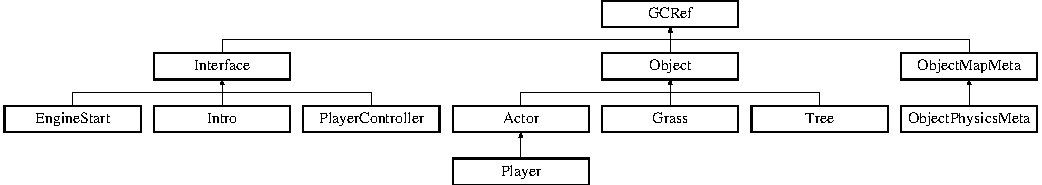
\includegraphics[height=2.480620cm]{classGCRef}
\end{center}
\end{figure}
\subsection*{Public Member Functions}
\begin{DoxyCompactItemize}
\item 
\hyperlink{classGCRefLink}{G\+C\+Ref\+Link} $\ast$ \hyperlink{classGCRef_ae39bea73b9c6af4a0df6ff490f3e8fa9}{link} ()
\begin{DoxyCompactList}\small\item\em link Get new link to indicate data usage \end{DoxyCompactList}\item 
\hypertarget{classGCRef_a7d1570b675959b895736d490d5998269}{}void \hyperlink{classGCRef_a7d1570b675959b895736d490d5998269}{unlock} ()\label{classGCRef_a7d1570b675959b895736d490d5998269}

\begin{DoxyCompactList}\small\item\em unlock Manually unlocks object \end{DoxyCompactList}\item 
int \hyperlink{classGCRef_a7cc24acd7029926613e9681e16f2bf76}{ref\+Users\+Count} () const 
\begin{DoxyCompactList}\small\item\em ref\+Users\+Count Returns current number of registered links \end{DoxyCompactList}\end{DoxyCompactItemize}
\subsection*{Friends}
\begin{DoxyCompactItemize}
\item 
\hypertarget{classGCRef_a697d68cbe829f48815533b70e888f1e6}{}class {\bfseries G\+C\+Ref\+Link}\label{classGCRef_a697d68cbe829f48815533b70e888f1e6}

\end{DoxyCompactItemize}


\subsection{Detailed Description}
The \hyperlink{classGCRef}{G\+C\+Ref} class Class providing basic garbage collecting functionality similar to one provided by sharedptr. 

User can get link which can be deleted later to inform that certain code won\textquotesingle{}t use data anymore. Once all links get deleted class is deleting itself on its own. New class has 0 links thus it\textquotesingle{}s locked. It can be manually unlocked, then deleted or it unlocks automatically after registering first link. 

\subsection{Member Function Documentation}
\hypertarget{classGCRef_ae39bea73b9c6af4a0df6ff490f3e8fa9}{}\index{G\+C\+Ref@{G\+C\+Ref}!link@{link}}
\index{link@{link}!G\+C\+Ref@{G\+C\+Ref}}
\subsubsection[{link}]{\setlength{\rightskip}{0pt plus 5cm}{\bf G\+C\+Ref\+Link} $\ast$ G\+C\+Ref\+::link (
\begin{DoxyParamCaption}
{}
\end{DoxyParamCaption}
)}\label{classGCRef_ae39bea73b9c6af4a0df6ff490f3e8fa9}


link Get new link to indicate data usage 

\begin{DoxyReturn}{Returns}
link 
\end{DoxyReturn}
\hypertarget{classGCRef_a7cc24acd7029926613e9681e16f2bf76}{}\index{G\+C\+Ref@{G\+C\+Ref}!ref\+Users\+Count@{ref\+Users\+Count}}
\index{ref\+Users\+Count@{ref\+Users\+Count}!G\+C\+Ref@{G\+C\+Ref}}
\subsubsection[{ref\+Users\+Count}]{\setlength{\rightskip}{0pt plus 5cm}int G\+C\+Ref\+::ref\+Users\+Count (
\begin{DoxyParamCaption}
{}
\end{DoxyParamCaption}
) const}\label{classGCRef_a7cc24acd7029926613e9681e16f2bf76}


ref\+Users\+Count Returns current number of registered links 

\begin{DoxyReturn}{Returns}
number of current users 
\end{DoxyReturn}


The documentation for this class was generated from the following files\+:\begin{DoxyCompactItemize}
\item 
include/utils.\+h\item 
src/utils.\+cpp\end{DoxyCompactItemize}

\hypertarget{classGCRefLink}{}\section{G\+C\+Ref\+Link Class Reference}
\label{classGCRefLink}\index{G\+C\+Ref\+Link@{G\+C\+Ref\+Link}}


The \hyperlink{classGCRefLink}{G\+C\+Ref\+Link} class Helper class to \hyperlink{classGCRefLink}{G\+C\+Ref\+Link}, once deleted -\/ \hyperlink{classGCRef}{G\+C\+Ref} class will unbind reference user and if it was last reference -\/ delete data.  




{\ttfamily \#include $<$utils.\+h$>$}

\subsection*{Friends}
\begin{DoxyCompactItemize}
\item 
\hypertarget{classGCRefLink_a85a14a8d83e08e75d136a7adf7d8da1d}{}class {\bfseries G\+C\+Ref}\label{classGCRefLink_a85a14a8d83e08e75d136a7adf7d8da1d}

\end{DoxyCompactItemize}


\subsection{Detailed Description}
The \hyperlink{classGCRefLink}{G\+C\+Ref\+Link} class Helper class to \hyperlink{classGCRefLink}{G\+C\+Ref\+Link}, once deleted -\/ \hyperlink{classGCRef}{G\+C\+Ref} class will unbind reference user and if it was last reference -\/ delete data. 

\begin{DoxySeeAlso}{See also}
\hyperlink{classGCRef}{G\+C\+Ref} 
\end{DoxySeeAlso}


The documentation for this class was generated from the following files\+:\begin{DoxyCompactItemize}
\item 
include/utils.\+h\item 
src/utils.\+cpp\end{DoxyCompactItemize}

\hypertarget{classGrass}{}\section{Grass Class Reference}
\label{classGrass}\index{Grass@{Grass}}
Inheritance diagram for Grass\+:\begin{figure}[H]
\begin{center}
\leavevmode
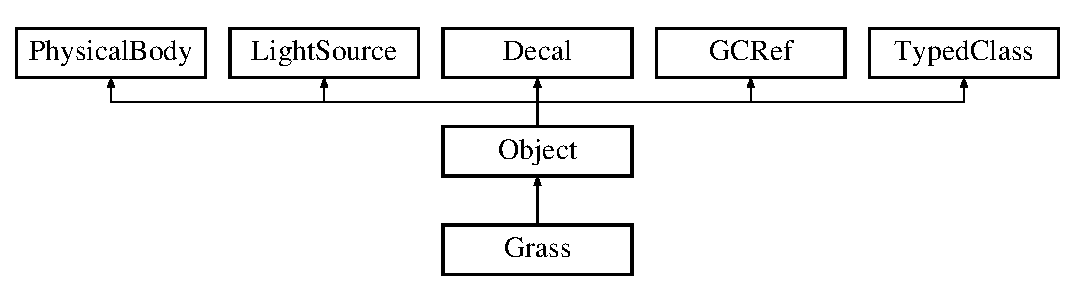
\includegraphics[height=3.000000cm]{classGrass}
\end{center}
\end{figure}
\subsection*{Public Member Functions}
\begin{DoxyCompactItemize}
\item 
\hypertarget{classGrass_a09378b8347074a59fe6a5485a174841a}{}{\bfseries Grass} (std\+::string n=\char`\"{}Grass\char`\"{})\label{classGrass_a09378b8347074a59fe6a5485a174841a}

\end{DoxyCompactItemize}
\subsection*{Static Public Attributes}
\begin{DoxyCompactItemize}
\item 
\hypertarget{classGrass_a4c182f101c0eff9c9e1178bcf52f13af}{}static constexpr char $\ast$ {\bfseries type\+Name} =(char$\ast$)\char`\"{}Grass\char`\"{}\label{classGrass_a4c182f101c0eff9c9e1178bcf52f13af}

\end{DoxyCompactItemize}
\subsection*{Additional Inherited Members}


The documentation for this class was generated from the following files\+:\begin{DoxyCompactItemize}
\item 
drivers/include/Static.\+h\item 
drivers/src/Static.\+cpp\end{DoxyCompactItemize}

\hypertarget{structPhysicsEngine_1_1CollisionGrid_1_1GridPool}{}\section{Physics\+Engine\+:\+:Collision\+Grid\+:\+:Grid\+Pool Struct Reference}
\label{structPhysicsEngine_1_1CollisionGrid_1_1GridPool}\index{Physics\+Engine\+::\+Collision\+Grid\+::\+Grid\+Pool@{Physics\+Engine\+::\+Collision\+Grid\+::\+Grid\+Pool}}


$<$ grid pool entry  




{\ttfamily \#include $<$physx.\+h$>$}

\subsection*{Public Attributes}
\begin{DoxyCompactItemize}
\item 
\hypertarget{structPhysicsEngine_1_1CollisionGrid_1_1GridPool_acf5494022e0a7eca8d00d46c6e43c834}{}int {\bfseries pos\+X}\label{structPhysicsEngine_1_1CollisionGrid_1_1GridPool_acf5494022e0a7eca8d00d46c6e43c834}

\item 
\hypertarget{structPhysicsEngine_1_1CollisionGrid_1_1GridPool_a51161a1c55352d84bd7e0812ba996d5e}{}int {\bfseries pos\+Y}\label{structPhysicsEngine_1_1CollisionGrid_1_1GridPool_a51161a1c55352d84bd7e0812ba996d5e}

\item 
\hypertarget{structPhysicsEngine_1_1CollisionGrid_1_1GridPool_aa1ecde48801839a6f8c2b1b1ab45924a}{}int {\bfseries ind\+R}\label{structPhysicsEngine_1_1CollisionGrid_1_1GridPool_aa1ecde48801839a6f8c2b1b1ab45924a}

\item 
\hypertarget{structPhysicsEngine_1_1CollisionGrid_1_1GridPool_a9c88faa1afccad9de3594a8423247304}{}int {\bfseries ind\+C}\label{structPhysicsEngine_1_1CollisionGrid_1_1GridPool_a9c88faa1afccad9de3594a8423247304}

\item 
\hypertarget{structPhysicsEngine_1_1CollisionGrid_1_1GridPool_a43d308da68b4d33e19365f95717594b6}{}\hyperlink{classChain}{Chain}$<$ \hyperlink{classObjectPhysicsMeta}{Object\+Physics\+Meta} $\ast$ $>$ $\ast$ \hyperlink{structPhysicsEngine_1_1CollisionGrid_1_1GridPool_a43d308da68b4d33e19365f95717594b6}{objects\+Chain}\label{structPhysicsEngine_1_1CollisionGrid_1_1GridPool_a43d308da68b4d33e19365f95717594b6}

\begin{DoxyCompactList}\small\item\em list of objects in single sector \end{DoxyCompactList}\end{DoxyCompactItemize}


\subsection{Detailed Description}
$<$ grid pool entry 

The documentation for this struct was generated from the following file\+:\begin{DoxyCompactItemize}
\item 
include/physx.\+h\end{DoxyCompactItemize}

\hypertarget{classInterface}{}\section{Interface Class Reference}
\label{classInterface}\index{Interface@{Interface}}


The \hyperlink{classInterface}{Interface} class \hyperlink{classInterface}{Interface} to be implemented by all drivers.  




{\ttfamily \#include $<$Game\+Domain.\+h$>$}

Inheritance diagram for Interface\+:\begin{figure}[H]
\begin{center}
\leavevmode
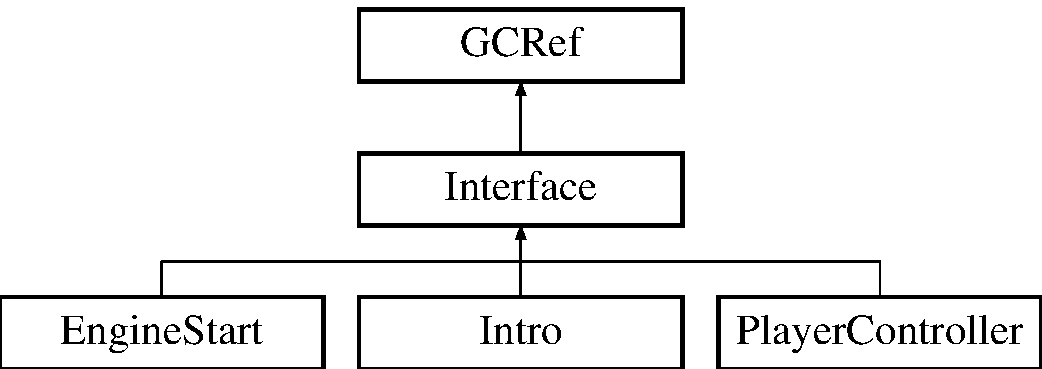
\includegraphics[height=3.000000cm]{classInterface}
\end{center}
\end{figure}
\subsection*{Public Member Functions}
\begin{DoxyCompactItemize}
\item 
virtual \hyperlink{classBaseEvent}{Base\+Event} \& \hyperlink{classInterface_addff25eb2adf4221c2be4895597b49c1}{run} (\hyperlink{classGameSession}{Game\+Session} \&session)=0
\begin{DoxyCompactList}\small\item\em run method called before each screen redraw \end{DoxyCompactList}\end{DoxyCompactItemize}


\subsection{Detailed Description}
The \hyperlink{classInterface}{Interface} class \hyperlink{classInterface}{Interface} to be implemented by all drivers. 

Each driver needs to implement certain functionality in order to work with game domain manager and session properly. \hyperlink{classInterface}{Interface} by default inherits from \hyperlink{classGCRef}{G\+C\+Ref} so it\textquotesingle{}s deleted automatically once all sessions using driver will be destroyed 

\subsection{Member Function Documentation}
\hypertarget{classInterface_addff25eb2adf4221c2be4895597b49c1}{}\index{Interface@{Interface}!run@{run}}
\index{run@{run}!Interface@{Interface}}
\subsubsection[{run}]{\setlength{\rightskip}{0pt plus 5cm}virtual {\bf Base\+Event}\& Interface\+::run (
\begin{DoxyParamCaption}
\item[{{\bf Game\+Session} \&}]{session}
\end{DoxyParamCaption}
)\hspace{0.3cm}{\ttfamily [pure virtual]}}\label{classInterface_addff25eb2adf4221c2be4895597b49c1}


run method called before each screen redraw 


\begin{DoxyParams}{Parameters}
{\em session} & current session passed to driver by game domain manager \\
\hline
\end{DoxyParams}
\begin{DoxyReturn}{Returns}

\end{DoxyReturn}


Implemented in \hyperlink{classEngineStart_a9caa9db3213371e5a77f1b09576a04fa}{Engine\+Start}, \hyperlink{classPlayerController_a062dc3debb7d14f2fc755b1b44ae7d07}{Player\+Controller}, and \hyperlink{classIntro_a3a8f112a89ee8c03e481910173ed5a33}{Intro}.



The documentation for this class was generated from the following files\+:\begin{DoxyCompactItemize}
\item 
include/Game\+Domain.\+h\item 
src/Game\+Domain.\+cpp\end{DoxyCompactItemize}

\hypertarget{classIntro}{}\section{Intro Class Reference}
\label{classIntro}\index{Intro@{Intro}}


The \hyperlink{classIntro}{Intro} Class is a tool which help us to control a session.  




{\ttfamily \#include $<$Intro.\+h$>$}

Inheritance diagram for Intro\+:\begin{figure}[H]
\begin{center}
\leavevmode
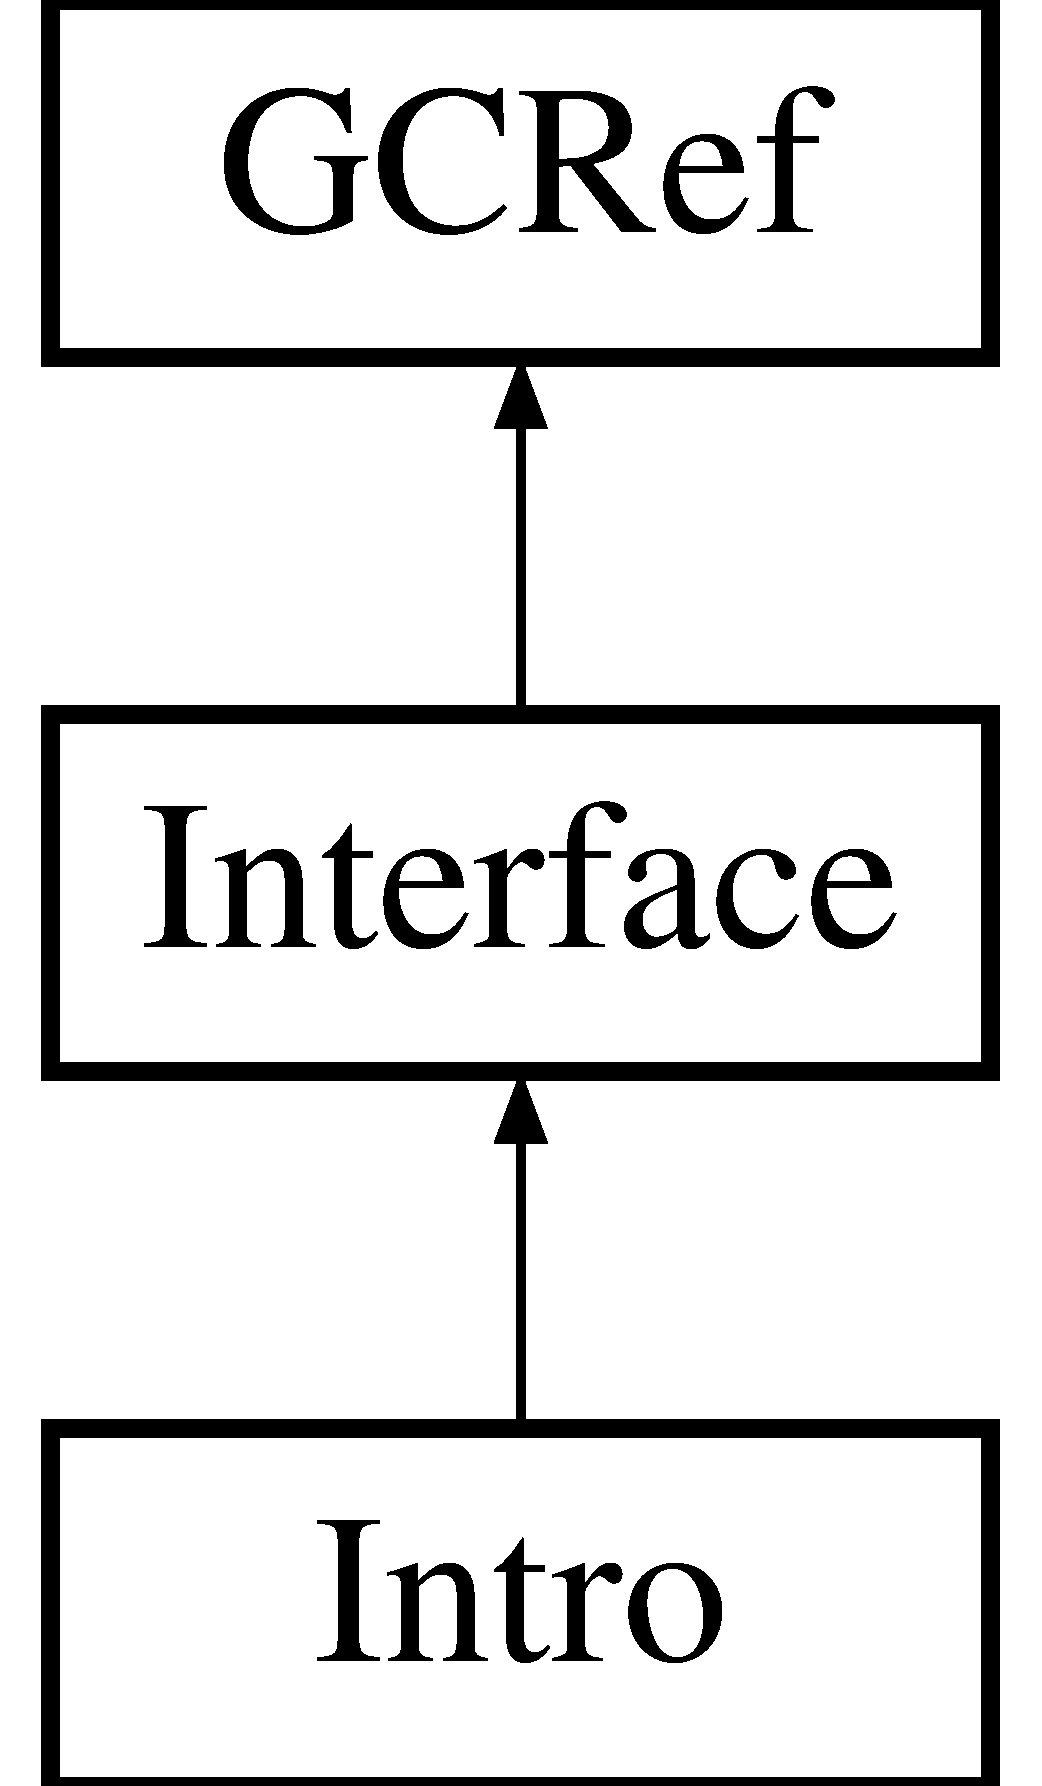
\includegraphics[height=3.000000cm]{classIntro}
\end{center}
\end{figure}
\subsection*{Public Member Functions}
\begin{DoxyCompactItemize}
\item 
\hyperlink{classBaseEvent}{Base\+Event} \& \hyperlink{classIntro_a3a8f112a89ee8c03e481910173ed5a33}{run} (\hyperlink{classGameSession}{Game\+Session} \&session)
\begin{DoxyCompactList}\small\item\em Basic funtion which control a session. \end{DoxyCompactList}\end{DoxyCompactItemize}


\subsection{Detailed Description}
The \hyperlink{classIntro}{Intro} Class is a tool which help us to control a session. 

This Class will change a current session to new one created in function.

\begin{DoxySeeAlso}{See also}
\hyperlink{classInterface}{Interface} 
\end{DoxySeeAlso}


\subsection{Member Function Documentation}
\hypertarget{classIntro_a3a8f112a89ee8c03e481910173ed5a33}{}\index{Intro@{Intro}!run@{run}}
\index{run@{run}!Intro@{Intro}}
\subsubsection[{run}]{\setlength{\rightskip}{0pt plus 5cm}{\bf Base\+Event} \& Intro\+::run (
\begin{DoxyParamCaption}
\item[{{\bf Game\+Session} \&}]{session}
\end{DoxyParamCaption}
)\hspace{0.3cm}{\ttfamily [virtual]}}\label{classIntro_a3a8f112a89ee8c03e481910173ed5a33}


Basic funtion which control a session. 

D\+O\+D\+A\+J\+E K\+L\+O\+C\+E\+K K\+T\+O\+R\+Y P\+O\+W\+I\+N\+I\+E\+N S\+T\+E\+R\+O\+W\+A\+C G\+R\+A\+C\+Z\+E\+M 

Implements \hyperlink{classInterface_addff25eb2adf4221c2be4895597b49c1}{Interface}.



The documentation for this class was generated from the following files\+:\begin{DoxyCompactItemize}
\item 
drivers/include/Intro.\+h\item 
drivers/src/Intro.\+cpp\end{DoxyCompactItemize}

\hypertarget{classLightSource}{}\section{Light\+Source Class Reference}
\label{classLightSource}\index{Light\+Source@{Light\+Source}}


The \hyperlink{classLightSource}{Light\+Source} class unimplemented.  




{\ttfamily \#include $<$object.\+h$>$}

Inheritance diagram for Light\+Source\+:\begin{figure}[H]
\begin{center}
\leavevmode
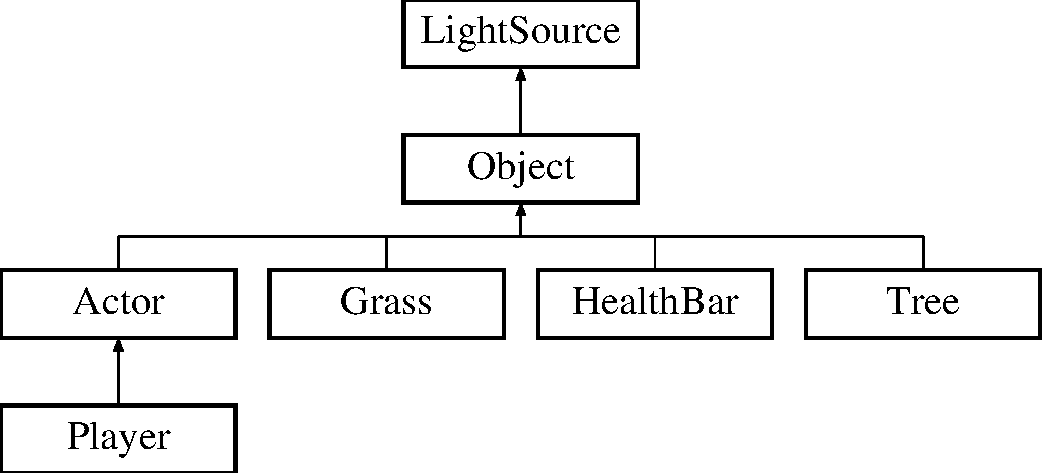
\includegraphics[height=4.000000cm]{classLightSource}
\end{center}
\end{figure}


\subsection{Detailed Description}
The \hyperlink{classLightSource}{Light\+Source} class unimplemented. 

The documentation for this class was generated from the following file\+:\begin{DoxyCompactItemize}
\item 
include/object.\+h\end{DoxyCompactItemize}

\hypertarget{classObject}{}\section{Object Class Reference}
\label{classObject}\index{Object@{Object}}


The \hyperlink{classObject}{Object} class Basic object class.  




{\ttfamily \#include $<$object.\+h$>$}

Inheritance diagram for Object\+:\begin{figure}[H]
\begin{center}
\leavevmode
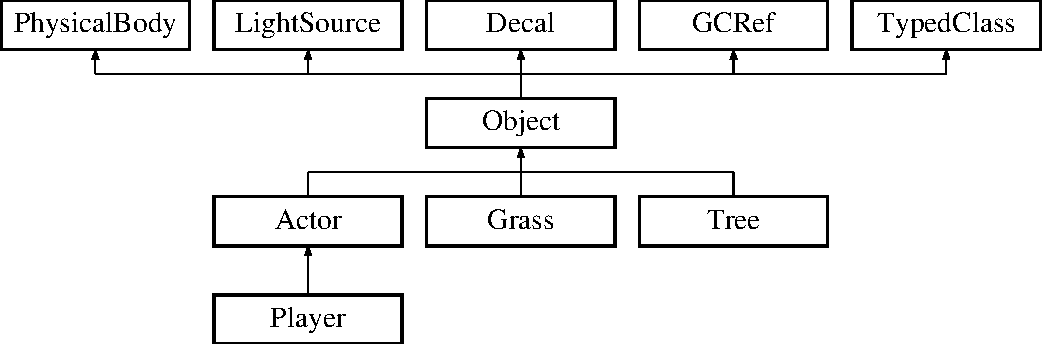
\includegraphics[height=4.000000cm]{classObject}
\end{center}
\end{figure}
\subsection*{Public Member Functions}
\begin{DoxyCompactItemize}
\item 
\hyperlink{classObject_af6520fb8cac84e70aec3ea95a88a31db}{Object} (const std\+::string name=std\+::string(\char`\"{}Object\char`\"{}), const \hyperlink{classDecal}{Decal} \&=\hyperlink{classDecal}{Decal}(), const \hyperlink{classPhysicalBody}{Physical\+Body} \&=\hyperlink{classPhysicalBody}{Physical\+Body}(Physical\+Body\+::\+Object\+Type\+::passive, Physical\+Body\+::\+Collision\+Type\+::ghost, \hyperlink{classPointXY}{Point\+X\+Y}(0, 0)), const \hyperlink{classLightSource}{Light\+Source} \&=\hyperlink{classLightSource}{Light\+Source}())
\begin{DoxyCompactList}\small\item\em \hyperlink{classObject}{Object} \hyperlink{classObject}{Object} constructor. \end{DoxyCompactList}\item 
\hyperlink{classObject_ade44910f4febbfdf035f3e33cfdb8af8}{Object} (const \hyperlink{classObject}{Object} \&ref)
\begin{DoxyCompactList}\small\item\em \hyperlink{classObject}{Object} Copy constructor. \end{DoxyCompactList}\item 
const std\+::string \hyperlink{classObject_a684b557e9a8f93987298ffa45beda51c}{get\+Name} () const 
\begin{DoxyCompactList}\small\item\em get\+Name \end{DoxyCompactList}\item 
bool \hyperlink{classObject_ac91f3c50f6cd45557836cf52d29ea03f}{operator==} (const \hyperlink{classObject}{Object} \&o) const 
\begin{DoxyCompactList}\small\item\em operator == compare operator \end{DoxyCompactList}\item 
bool \hyperlink{classObject_a93e19069474d6fdd44c744282f4ffe27}{operator!=} (const \hyperlink{classObject}{Object} \&o) const 
\begin{DoxyCompactList}\small\item\em operator != compare operator \end{DoxyCompactList}\end{DoxyCompactItemize}
\subsection*{Static Public Attributes}
\begin{DoxyCompactItemize}
\item 
\hypertarget{classObject_add9e5b23ab163db74d191ed7fe5b7f70}{}static constexpr char $\ast$ \hyperlink{classObject_add9e5b23ab163db74d191ed7fe5b7f70}{type\+Name} =(char$\ast$)\char`\"{}Object\char`\"{}\label{classObject_add9e5b23ab163db74d191ed7fe5b7f70}

\begin{DoxyCompactList}\small\item\em object type name \end{DoxyCompactList}\item 
\hypertarget{classObject_ad72b7e373242e30424c4affc2bf74497}{}static const \hyperlink{classObject}{Object} \hyperlink{classObject_ad72b7e373242e30424c4affc2bf74497}{null\+Obj} =\hyperlink{classObject}{Object}()\label{classObject_ad72b7e373242e30424c4affc2bf74497}

\begin{DoxyCompactList}\small\item\em dummy object for placeholder purpose \end{DoxyCompactList}\end{DoxyCompactItemize}
\subsection*{Additional Inherited Members}


\subsection{Detailed Description}
The \hyperlink{classObject}{Object} class Basic object class. 

\subsection{Constructor \& Destructor Documentation}
\hypertarget{classObject_af6520fb8cac84e70aec3ea95a88a31db}{}\index{Object@{Object}!Object@{Object}}
\index{Object@{Object}!Object@{Object}}
\subsubsection[{Object}]{\setlength{\rightskip}{0pt plus 5cm}Object\+::\+Object (
\begin{DoxyParamCaption}
\item[{const std\+::string}]{name = {\ttfamily std\+:\+:string(\char`\"{}Object\char`\"{})}, }
\item[{const {\bf Decal} \&}]{decal = {\ttfamily {\bf Decal}()}, }
\item[{const {\bf Physical\+Body} \&}]{physical\+Body = {\ttfamily {\bf Physical\+Body}(PhysicalBody\+:\+:ObjectType\+:\+:passive,~PhysicalBody\+:\+:CollisionType\+:\+:ghost,~{\bf Point\+X\+Y}(0,0))}, }
\item[{const {\bf Light\+Source} \&}]{light\+Source = {\ttfamily {\bf Light\+Source}()}}
\end{DoxyParamCaption}
)}\label{classObject_af6520fb8cac84e70aec3ea95a88a31db}


\hyperlink{classObject}{Object} \hyperlink{classObject}{Object} constructor. 


\begin{DoxyParams}{Parameters}
{\em name} & name of new \hyperlink{classObject}{Object}. Can be used by game domain code \\
\hline
\end{DoxyParams}
\hypertarget{classObject_ade44910f4febbfdf035f3e33cfdb8af8}{}\index{Object@{Object}!Object@{Object}}
\index{Object@{Object}!Object@{Object}}
\subsubsection[{Object}]{\setlength{\rightskip}{0pt plus 5cm}Object\+::\+Object (
\begin{DoxyParamCaption}
\item[{const {\bf Object} \&}]{ref}
\end{DoxyParamCaption}
)}\label{classObject_ade44910f4febbfdf035f3e33cfdb8af8}


\hyperlink{classObject}{Object} Copy constructor. 


\begin{DoxyParams}{Parameters}
{\em ref} & reference object \\
\hline
\end{DoxyParams}


\subsection{Member Function Documentation}
\hypertarget{classObject_a684b557e9a8f93987298ffa45beda51c}{}\index{Object@{Object}!get\+Name@{get\+Name}}
\index{get\+Name@{get\+Name}!Object@{Object}}
\subsubsection[{get\+Name}]{\setlength{\rightskip}{0pt plus 5cm}const std\+::string Object\+::get\+Name (
\begin{DoxyParamCaption}
{}
\end{DoxyParamCaption}
) const\hspace{0.3cm}{\ttfamily [inline]}}\label{classObject_a684b557e9a8f93987298ffa45beda51c}


get\+Name 

\begin{DoxyReturn}{Returns}
name of object 
\end{DoxyReturn}
\hypertarget{classObject_a93e19069474d6fdd44c744282f4ffe27}{}\index{Object@{Object}!operator"!=@{operator"!=}}
\index{operator"!=@{operator"!=}!Object@{Object}}
\subsubsection[{operator"!=}]{\setlength{\rightskip}{0pt plus 5cm}bool Object\+::operator!= (
\begin{DoxyParamCaption}
\item[{const {\bf Object} \&}]{o}
\end{DoxyParamCaption}
) const\hspace{0.3cm}{\ttfamily [inline]}}\label{classObject_a93e19069474d6fdd44c744282f4ffe27}


operator != compare operator 


\begin{DoxyParams}{Parameters}
{\em o} & \\
\hline
\end{DoxyParams}
\begin{DoxyReturn}{Returns}

\end{DoxyReturn}
\hypertarget{classObject_ac91f3c50f6cd45557836cf52d29ea03f}{}\index{Object@{Object}!operator==@{operator==}}
\index{operator==@{operator==}!Object@{Object}}
\subsubsection[{operator==}]{\setlength{\rightskip}{0pt plus 5cm}bool Object\+::operator== (
\begin{DoxyParamCaption}
\item[{const {\bf Object} \&}]{o}
\end{DoxyParamCaption}
) const\hspace{0.3cm}{\ttfamily [inline]}}\label{classObject_ac91f3c50f6cd45557836cf52d29ea03f}


operator == compare operator 


\begin{DoxyParams}{Parameters}
{\em o} & \\
\hline
\end{DoxyParams}
\begin{DoxyReturn}{Returns}

\end{DoxyReturn}


The documentation for this class was generated from the following files\+:\begin{DoxyCompactItemize}
\item 
include/object.\+h\item 
src/object.\+cpp\end{DoxyCompactItemize}

\hypertarget{classObjectMapMeta}{}\section{Object\+Map\+Meta Class Reference}
\label{classObjectMapMeta}\index{Object\+Map\+Meta@{Object\+Map\+Meta}}


The \hyperlink{classObjectMapMeta}{Object\+Map\+Meta} class \hyperlink{classObject}{Object} meta class containing map-\/related properties of object.  




{\ttfamily \#include $<$map.\+h$>$}

Inheritance diagram for Object\+Map\+Meta\+:\begin{figure}[H]
\begin{center}
\leavevmode
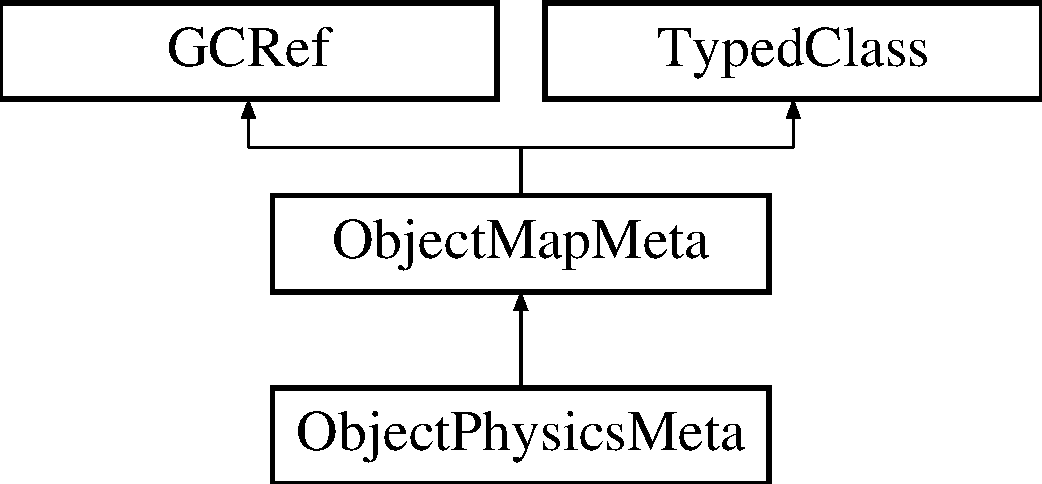
\includegraphics[height=3.000000cm]{classObjectMapMeta}
\end{center}
\end{figure}
\subsection*{Public Member Functions}
\begin{DoxyCompactItemize}
\item 
\hyperlink{classObjectMapMeta_a5217b0d2a08ec5ed88f790c9f75a0b75}{Object\+Map\+Meta} (\hyperlink{classObject}{Object} \&obj, \hyperlink{classPointXY}{Point\+X\+Y} \hyperlink{classObjectMapMeta_a7ca5609abb6c5fd57fe3828725240847}{pos}=\hyperlink{classPointXY}{Point\+X\+Y}(0, 0))
\begin{DoxyCompactList}\small\item\em \hyperlink{classObjectMapMeta}{Object\+Map\+Meta} Constructor. \end{DoxyCompactList}\item 
\hyperlink{classObjectMapMeta_a97778bafcdef8809112e315189371045}{Object\+Map\+Meta} (const \hyperlink{classObjectMapMeta}{Object\+Map\+Meta} \&ref)
\begin{DoxyCompactList}\small\item\em \hyperlink{classObjectMapMeta}{Object\+Map\+Meta} copy constructor. \end{DoxyCompactList}\item 
\hyperlink{classObjectMapMeta}{Object\+Map\+Meta} $\ast$ \hyperlink{classObjectMapMeta_a01202e363d84edbcb7b301c97400dd58}{get\+Anchor} () const 
\begin{DoxyCompactList}\small\item\em get\+Anchor returns parent object which meta is attached to \end{DoxyCompactList}\item 
\hyperlink{classObjectMapMeta}{Object\+Map\+Meta} $\ast$ \hyperlink{classObjectMapMeta_a50cb677227ba335c397b24bd170f032d}{get\+Tail} () const 
\begin{DoxyCompactList}\small\item\em get\+Tail returns child object which is attached to this object \end{DoxyCompactList}\item 
\hyperlink{classObjectMapMeta}{Object\+Map\+Meta} $\ast$ \hyperlink{classObjectMapMeta_ae8dd47a6811d0244dc3f10991a749569}{get\+Root} () const 
\begin{DoxyCompactList}\small\item\em get\+Root returns topmost parent in objects hierarchy \end{DoxyCompactList}\item 
\hyperlink{classPointXY}{Point\+X\+Y} \hyperlink{classObjectMapMeta_a66b92b6e542b4170a3a2c830d95807d8}{get\+Global\+Pos} () const 
\begin{DoxyCompactList}\small\item\em get\+Global\+Pos returns calculated global position (affected by \end{DoxyCompactList}\item 
void \hyperlink{classObjectMapMeta_ae4a20414fe790ad32542294d18efb931}{attach} (\hyperlink{classObjectMapMeta}{Object\+Map\+Meta} \&anchor)
\begin{DoxyCompactList}\small\item\em attach Attaches object to another one \end{DoxyCompactList}\item 
\hypertarget{classObjectMapMeta_ab73aa1e8a6cb41fcedc94ebf904a5c41}{}void \hyperlink{classObjectMapMeta_ab73aa1e8a6cb41fcedc94ebf904a5c41}{detach} ()\label{classObjectMapMeta_ab73aa1e8a6cb41fcedc94ebf904a5c41}

\begin{DoxyCompactList}\small\item\em detach Detaches object from parent \end{DoxyCompactList}\item 
bool \hyperlink{classObjectMapMeta_ac0ba6c1b3c98a0b015e60da4575411cb}{is\+In\+Use} () const 
\begin{DoxyCompactList}\small\item\em is\+In\+Use Indicates whether meta is already placed on map or not \end{DoxyCompactList}\item 
\hyperlink{classGameMap}{Game\+Map} $\ast$ \hyperlink{classObjectMapMeta_ae9a94a068918c364af21c8e8dc515f0a}{get\+Map} () const 
\begin{DoxyCompactList}\small\item\em get\+Map returns map which object is placed on \end{DoxyCompactList}\end{DoxyCompactItemize}
\subsection*{Public Attributes}
\begin{DoxyCompactItemize}
\item 
\hypertarget{classObjectMapMeta_a7c63160bc0d55ce0dfa9819a5796e027}{}\hyperlink{classObject}{Object} \& \hyperlink{classObjectMapMeta_a7c63160bc0d55ce0dfa9819a5796e027}{object}\label{classObjectMapMeta_a7c63160bc0d55ce0dfa9819a5796e027}

\begin{DoxyCompactList}\small\item\em represented object reference \end{DoxyCompactList}\item 
\hypertarget{classObjectMapMeta_a7ca5609abb6c5fd57fe3828725240847}{}\hyperlink{classPointXY}{Point\+X\+Y} \hyperlink{classObjectMapMeta_a7ca5609abb6c5fd57fe3828725240847}{pos}\label{classObjectMapMeta_a7ca5609abb6c5fd57fe3828725240847}

\begin{DoxyCompactList}\small\item\em object position or offset from anchor (parent) \end{DoxyCompactList}\end{DoxyCompactItemize}
\subsection*{Static Public Attributes}
\begin{DoxyCompactItemize}
\item 
\hypertarget{classObjectMapMeta_a65628ecfd0b0db1e2e2534d2ed93a59b}{}static constexpr char $\ast$ \hyperlink{classObjectMapMeta_a65628ecfd0b0db1e2e2534d2ed93a59b}{type\+Name} =(char$\ast$)\char`\"{}Meta\char`\"{}\label{classObjectMapMeta_a65628ecfd0b0db1e2e2534d2ed93a59b}

\begin{DoxyCompactList}\small\item\em type name \end{DoxyCompactList}\end{DoxyCompactItemize}
\subsection*{Protected Member Functions}
\begin{DoxyCompactItemize}
\item 
\hypertarget{classObjectMapMeta_a80a10a6a51b8533c24f5106d3be695d5}{}virtual void {\bfseries link\+Map} (\hyperlink{classGameMap}{Game\+Map} \&map)\label{classObjectMapMeta_a80a10a6a51b8533c24f5106d3be695d5}

\item 
\hypertarget{classObjectMapMeta_a3b256fc24b4c5262443094634a91330c}{}virtual void {\bfseries unlink\+Map} ()\label{classObjectMapMeta_a3b256fc24b4c5262443094634a91330c}

\end{DoxyCompactItemize}
\subsection*{Protected Attributes}
\begin{DoxyCompactItemize}
\item 
\hypertarget{classObjectMapMeta_a4dd5cbfe0d5de2020a432f3deb94bbb2}{}bool {\bfseries in\+Use}\label{classObjectMapMeta_a4dd5cbfe0d5de2020a432f3deb94bbb2}

\item 
\hypertarget{classObjectMapMeta_a97d9c262d487cce070f22f035f1c1e16}{}\hyperlink{classGCRefLink}{G\+C\+Ref\+Link} $\ast$ {\bfseries map\+Link}\label{classObjectMapMeta_a97d9c262d487cce070f22f035f1c1e16}

\item 
\hypertarget{classObjectMapMeta_aec01f78a915fd54a8cf7ba59de3d3dcf}{}\hyperlink{classGameMap}{Game\+Map} $\ast$ {\bfseries map}\label{classObjectMapMeta_aec01f78a915fd54a8cf7ba59de3d3dcf}

\end{DoxyCompactItemize}
\subsection*{Friends}
\begin{DoxyCompactItemize}
\item 
\hypertarget{classObjectMapMeta_a93630ea74a3218a3e2e96b7bf2c07c66}{}class {\bfseries Game\+Map}\label{classObjectMapMeta_a93630ea74a3218a3e2e96b7bf2c07c66}

\end{DoxyCompactItemize}


\subsection{Detailed Description}
The \hyperlink{classObjectMapMeta}{Object\+Map\+Meta} class \hyperlink{classObject}{Object} meta class containing map-\/related properties of object. 

\hyperlink{classObjectMapMeta}{Object\+Map\+Meta} class provides map-\/specific properties related to object like various relations between objects (attachment of one object to another) and position. Single \hyperlink{classObject}{Object} can be placed multiple times on single map using multiple \hyperlink{classObjectMapMeta}{Object\+Map\+Meta} instances, however it\textquotesingle{}ll literally link instances of object on map, thus any operations performed on original object except map-\/specific properties will affect both of them. Useful for template and non-\/interactive objects which can be placed in many places on single map

\begin{DoxySeeAlso}{See also}
\hyperlink{classGameMap}{Game\+Map} 

\hyperlink{classObjectPhysicsMeta}{Object\+Physics\+Meta} 
\end{DoxySeeAlso}


\subsection{Constructor \& Destructor Documentation}
\hypertarget{classObjectMapMeta_a5217b0d2a08ec5ed88f790c9f75a0b75}{}\index{Object\+Map\+Meta@{Object\+Map\+Meta}!Object\+Map\+Meta@{Object\+Map\+Meta}}
\index{Object\+Map\+Meta@{Object\+Map\+Meta}!Object\+Map\+Meta@{Object\+Map\+Meta}}
\subsubsection[{Object\+Map\+Meta}]{\setlength{\rightskip}{0pt plus 5cm}Object\+Map\+Meta\+::\+Object\+Map\+Meta (
\begin{DoxyParamCaption}
\item[{{\bf Object} \&}]{obj, }
\item[{{\bf Point\+X\+Y}}]{pos = {\ttfamily {\bf Point\+X\+Y}(0,0)}}
\end{DoxyParamCaption}
)}\label{classObjectMapMeta_a5217b0d2a08ec5ed88f790c9f75a0b75}


\hyperlink{classObjectMapMeta}{Object\+Map\+Meta} Constructor. 


\begin{DoxyParams}{Parameters}
{\em obj} & represented object \\
\hline
{\em pos} & initial position \\
\hline
\end{DoxyParams}
\hypertarget{classObjectMapMeta_a97778bafcdef8809112e315189371045}{}\index{Object\+Map\+Meta@{Object\+Map\+Meta}!Object\+Map\+Meta@{Object\+Map\+Meta}}
\index{Object\+Map\+Meta@{Object\+Map\+Meta}!Object\+Map\+Meta@{Object\+Map\+Meta}}
\subsubsection[{Object\+Map\+Meta}]{\setlength{\rightskip}{0pt plus 5cm}Object\+Map\+Meta\+::\+Object\+Map\+Meta (
\begin{DoxyParamCaption}
\item[{const {\bf Object\+Map\+Meta} \&}]{ref}
\end{DoxyParamCaption}
)}\label{classObjectMapMeta_a97778bafcdef8809112e315189371045}


\hyperlink{classObjectMapMeta}{Object\+Map\+Meta} copy constructor. 


\begin{DoxyParams}{Parameters}
{\em ref} & reference meta \\
\hline
\end{DoxyParams}


\subsection{Member Function Documentation}
\hypertarget{classObjectMapMeta_ae4a20414fe790ad32542294d18efb931}{}\index{Object\+Map\+Meta@{Object\+Map\+Meta}!attach@{attach}}
\index{attach@{attach}!Object\+Map\+Meta@{Object\+Map\+Meta}}
\subsubsection[{attach}]{\setlength{\rightskip}{0pt plus 5cm}void Object\+Map\+Meta\+::attach (
\begin{DoxyParamCaption}
\item[{{\bf Object\+Map\+Meta} \&}]{anchor}
\end{DoxyParamCaption}
)}\label{classObjectMapMeta_ae4a20414fe790ad32542294d18efb931}


attach Attaches object to another one 


\begin{DoxyParams}{Parameters}
{\em anchor} & new parent meta \\
\hline
\end{DoxyParams}
\hypertarget{classObjectMapMeta_a01202e363d84edbcb7b301c97400dd58}{}\index{Object\+Map\+Meta@{Object\+Map\+Meta}!get\+Anchor@{get\+Anchor}}
\index{get\+Anchor@{get\+Anchor}!Object\+Map\+Meta@{Object\+Map\+Meta}}
\subsubsection[{get\+Anchor}]{\setlength{\rightskip}{0pt plus 5cm}{\bf Object\+Map\+Meta}$\ast$ Object\+Map\+Meta\+::get\+Anchor (
\begin{DoxyParamCaption}
{}
\end{DoxyParamCaption}
) const\hspace{0.3cm}{\ttfamily [inline]}}\label{classObjectMapMeta_a01202e363d84edbcb7b301c97400dd58}


get\+Anchor returns parent object which meta is attached to 

\begin{DoxyReturn}{Returns}
parent meta 
\end{DoxyReturn}
\hypertarget{classObjectMapMeta_a66b92b6e542b4170a3a2c830d95807d8}{}\index{Object\+Map\+Meta@{Object\+Map\+Meta}!get\+Global\+Pos@{get\+Global\+Pos}}
\index{get\+Global\+Pos@{get\+Global\+Pos}!Object\+Map\+Meta@{Object\+Map\+Meta}}
\subsubsection[{get\+Global\+Pos}]{\setlength{\rightskip}{0pt plus 5cm}{\bf Point\+X\+Y} Object\+Map\+Meta\+::get\+Global\+Pos (
\begin{DoxyParamCaption}
{}
\end{DoxyParamCaption}
) const\hspace{0.3cm}{\ttfamily [inline]}}\label{classObjectMapMeta_a66b92b6e542b4170a3a2c830d95807d8}


get\+Global\+Pos returns calculated global position (affected by 

\begin{DoxyReturn}{Returns}

\end{DoxyReturn}
\hypertarget{classObjectMapMeta_ae9a94a068918c364af21c8e8dc515f0a}{}\index{Object\+Map\+Meta@{Object\+Map\+Meta}!get\+Map@{get\+Map}}
\index{get\+Map@{get\+Map}!Object\+Map\+Meta@{Object\+Map\+Meta}}
\subsubsection[{get\+Map}]{\setlength{\rightskip}{0pt plus 5cm}{\bf Game\+Map}$\ast$ Object\+Map\+Meta\+::get\+Map (
\begin{DoxyParamCaption}
{}
\end{DoxyParamCaption}
) const\hspace{0.3cm}{\ttfamily [inline]}}\label{classObjectMapMeta_ae9a94a068918c364af21c8e8dc515f0a}


get\+Map returns map which object is placed on 

\begin{DoxyReturn}{Returns}

\end{DoxyReturn}
\hypertarget{classObjectMapMeta_ae8dd47a6811d0244dc3f10991a749569}{}\index{Object\+Map\+Meta@{Object\+Map\+Meta}!get\+Root@{get\+Root}}
\index{get\+Root@{get\+Root}!Object\+Map\+Meta@{Object\+Map\+Meta}}
\subsubsection[{get\+Root}]{\setlength{\rightskip}{0pt plus 5cm}{\bf Object\+Map\+Meta}$\ast$ Object\+Map\+Meta\+::get\+Root (
\begin{DoxyParamCaption}
{}
\end{DoxyParamCaption}
) const\hspace{0.3cm}{\ttfamily [inline]}}\label{classObjectMapMeta_ae8dd47a6811d0244dc3f10991a749569}


get\+Root returns topmost parent in objects hierarchy 

\begin{DoxyReturn}{Returns}
topmost parent meta 
\end{DoxyReturn}
\hypertarget{classObjectMapMeta_a50cb677227ba335c397b24bd170f032d}{}\index{Object\+Map\+Meta@{Object\+Map\+Meta}!get\+Tail@{get\+Tail}}
\index{get\+Tail@{get\+Tail}!Object\+Map\+Meta@{Object\+Map\+Meta}}
\subsubsection[{get\+Tail}]{\setlength{\rightskip}{0pt plus 5cm}{\bf Object\+Map\+Meta}$\ast$ Object\+Map\+Meta\+::get\+Tail (
\begin{DoxyParamCaption}
{}
\end{DoxyParamCaption}
) const\hspace{0.3cm}{\ttfamily [inline]}}\label{classObjectMapMeta_a50cb677227ba335c397b24bd170f032d}


get\+Tail returns child object which is attached to this object 

\begin{DoxyReturn}{Returns}
child meta 
\end{DoxyReturn}
\hypertarget{classObjectMapMeta_ac0ba6c1b3c98a0b015e60da4575411cb}{}\index{Object\+Map\+Meta@{Object\+Map\+Meta}!is\+In\+Use@{is\+In\+Use}}
\index{is\+In\+Use@{is\+In\+Use}!Object\+Map\+Meta@{Object\+Map\+Meta}}
\subsubsection[{is\+In\+Use}]{\setlength{\rightskip}{0pt plus 5cm}bool Object\+Map\+Meta\+::is\+In\+Use (
\begin{DoxyParamCaption}
{}
\end{DoxyParamCaption}
) const\hspace{0.3cm}{\ttfamily [inline]}}\label{classObjectMapMeta_ac0ba6c1b3c98a0b015e60da4575411cb}


is\+In\+Use Indicates whether meta is already placed on map or not 

\begin{DoxyReturn}{Returns}

\end{DoxyReturn}


The documentation for this class was generated from the following files\+:\begin{DoxyCompactItemize}
\item 
include/map.\+h\item 
src/map.\+cpp\end{DoxyCompactItemize}

\hypertarget{classObjectPhysicsMeta}{}\section{Object\+Physics\+Meta Class Reference}
\label{classObjectPhysicsMeta}\index{Object\+Physics\+Meta@{Object\+Physics\+Meta}}


The \hyperlink{classObjectPhysicsMeta}{Object\+Physics\+Meta} class Extension to \hyperlink{classObjectMapMeta}{Object\+Map\+Meta} class adding physical properties like speed, acceleration...  




{\ttfamily \#include $<$physx.\+h$>$}

Inheritance diagram for Object\+Physics\+Meta\+:\begin{figure}[H]
\begin{center}
\leavevmode
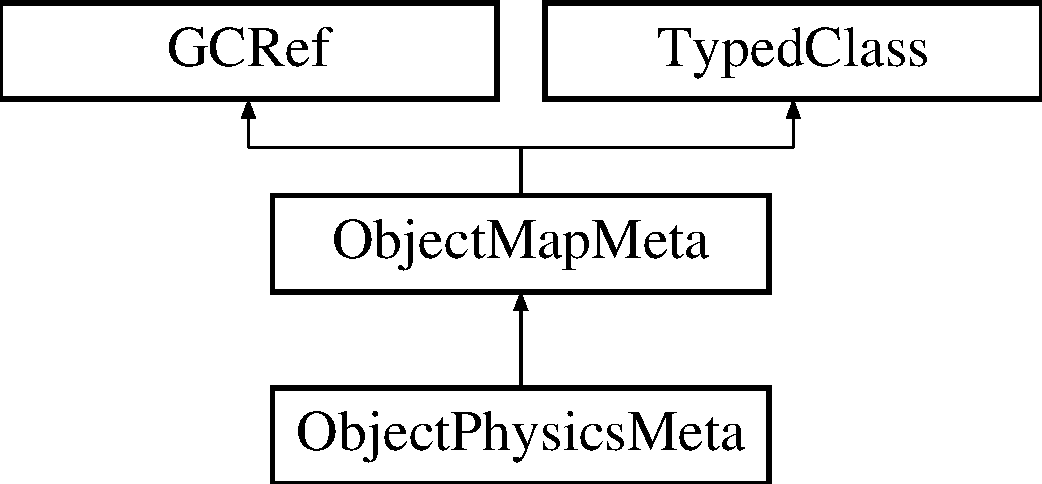
\includegraphics[height=3.000000cm]{classObjectPhysicsMeta}
\end{center}
\end{figure}
\subsection*{Public Member Functions}
\begin{DoxyCompactItemize}
\item 
\hyperlink{classObjectPhysicsMeta_a5f9da87e92c7d03ba1213542f5d7a6c6}{Object\+Physics\+Meta} (const \hyperlink{classObjectMapMeta}{Object\+Map\+Meta} \&ref, const \hyperlink{classPhysicsEngine}{Physics\+Engine} \&engine, \hyperlink{classVectorXY}{Vector\+X\+Y} \hyperlink{classObjectPhysicsMeta_a9d6fae5e4518766e715781227e3fb9a9}{speed}=\hyperlink{classVectorXY}{Vector\+X\+Y}(0, 0, 0, 0), \hyperlink{classVectorXY}{Vector\+X\+Y} \hyperlink{classObjectPhysicsMeta_ab2ef030e0178008c40520e615790a854}{acceleration}=\hyperlink{classVectorXY}{Vector\+X\+Y}(0, 0, 0, 0))
\begin{DoxyCompactList}\small\item\em \hyperlink{classObjectPhysicsMeta}{Object\+Physics\+Meta} Constructor. \end{DoxyCompactList}\end{DoxyCompactItemize}
\subsection*{Public Attributes}
\begin{DoxyCompactItemize}
\item 
\hypertarget{classObjectPhysicsMeta_a9d6fae5e4518766e715781227e3fb9a9}{}\hyperlink{classVectorXY}{Vector\+X\+Y} \hyperlink{classObjectPhysicsMeta_a9d6fae5e4518766e715781227e3fb9a9}{speed}\label{classObjectPhysicsMeta_a9d6fae5e4518766e715781227e3fb9a9}

\begin{DoxyCompactList}\small\item\em object speed \end{DoxyCompactList}\item 
\hypertarget{classObjectPhysicsMeta_ab2ef030e0178008c40520e615790a854}{}\hyperlink{classVectorXY}{Vector\+X\+Y} \hyperlink{classObjectPhysicsMeta_ab2ef030e0178008c40520e615790a854}{acceleration}\label{classObjectPhysicsMeta_ab2ef030e0178008c40520e615790a854}

\begin{DoxyCompactList}\small\item\em object acceleration \end{DoxyCompactList}\end{DoxyCompactItemize}
\subsection*{Static Public Attributes}
\begin{DoxyCompactItemize}
\item 
\hypertarget{classObjectPhysicsMeta_a6017a1245eb08ec3e829b2c1c08aeede}{}static constexpr char $\ast$ {\bfseries type\+Name} =(char$\ast$)\char`\"{}Physics\+Meta\char`\"{}\label{classObjectPhysicsMeta_a6017a1245eb08ec3e829b2c1c08aeede}

\end{DoxyCompactItemize}
\subsection*{Protected Member Functions}
\begin{DoxyCompactItemize}
\item 
\hypertarget{classObjectPhysicsMeta_a429712351080fbccba9fb32b11ab1072}{}virtual void {\bfseries link\+Map} (\hyperlink{classGameMap}{Game\+Map} \&map)\label{classObjectPhysicsMeta_a429712351080fbccba9fb32b11ab1072}

\item 
\hypertarget{classObjectPhysicsMeta_a5e391ee1abaa3e04d3961a1c1e51c73b}{}virtual void {\bfseries unlink\+Map} ()\label{classObjectPhysicsMeta_a5e391ee1abaa3e04d3961a1c1e51c73b}

\end{DoxyCompactItemize}
\subsection*{Friends}
\begin{DoxyCompactItemize}
\item 
\hypertarget{classObjectPhysicsMeta_a7d5d92b2453386482dd08e0908612a46}{}class {\bfseries Physics\+Engine\+::\+Collision\+Grid}\label{classObjectPhysicsMeta_a7d5d92b2453386482dd08e0908612a46}

\end{DoxyCompactItemize}
\subsection*{Additional Inherited Members}


\subsection{Detailed Description}
The \hyperlink{classObjectPhysicsMeta}{Object\+Physics\+Meta} class Extension to \hyperlink{classObjectMapMeta}{Object\+Map\+Meta} class adding physical properties like speed, acceleration... 

\begin{DoxySeeAlso}{See also}
\hyperlink{classObjectMapMeta}{Object\+Map\+Meta} 

\hyperlink{classPhysicsEngine}{Physics\+Engine} 
\end{DoxySeeAlso}


\subsection{Constructor \& Destructor Documentation}
\hypertarget{classObjectPhysicsMeta_a5f9da87e92c7d03ba1213542f5d7a6c6}{}\index{Object\+Physics\+Meta@{Object\+Physics\+Meta}!Object\+Physics\+Meta@{Object\+Physics\+Meta}}
\index{Object\+Physics\+Meta@{Object\+Physics\+Meta}!Object\+Physics\+Meta@{Object\+Physics\+Meta}}
\subsubsection[{Object\+Physics\+Meta}]{\setlength{\rightskip}{0pt plus 5cm}Object\+Physics\+Meta\+::\+Object\+Physics\+Meta (
\begin{DoxyParamCaption}
\item[{const {\bf Object\+Map\+Meta} \&}]{ref, }
\item[{const {\bf Physics\+Engine} \&}]{engine, }
\item[{{\bf Vector\+X\+Y}}]{speed = {\ttfamily {\bf Vector\+X\+Y}(0,0,0,0)}, }
\item[{{\bf Vector\+X\+Y}}]{acceleration = {\ttfamily {\bf Vector\+X\+Y}(0,0,0,0)}}
\end{DoxyParamCaption}
)}\label{classObjectPhysicsMeta_a5f9da87e92c7d03ba1213542f5d7a6c6}


\hyperlink{classObjectPhysicsMeta}{Object\+Physics\+Meta} Constructor. 


\begin{DoxyParams}{Parameters}
{\em ref} & reference meta to be converted to Physics meta \\
\hline
{\em engine} & engine to register in \\
\hline
{\em speed} & initial speed \\
\hline
{\em acceleration} & initial acceleration \\
\hline
\end{DoxyParams}


The documentation for this class was generated from the following files\+:\begin{DoxyCompactItemize}
\item 
include/physx.\+h\item 
src/physx.\+cpp\end{DoxyCompactItemize}

\hypertarget{structRenderEngine_1_1objRecord}{}\section{Render\+Engine\+:\+:obj\+Record Struct Reference}
\label{structRenderEngine_1_1objRecord}\index{Render\+Engine\+::obj\+Record@{Render\+Engine\+::obj\+Record}}
\subsection*{Public Attributes}
\begin{DoxyCompactItemize}
\item 
\hypertarget{structRenderEngine_1_1objRecord_a06402ecee09ee496ffa27ad16f621f05}{}\hyperlink{classPointXY}{Point\+X\+Y} {\bfseries pos}\label{structRenderEngine_1_1objRecord_a06402ecee09ee496ffa27ad16f621f05}

\item 
\hypertarget{structRenderEngine_1_1objRecord_addb8999769865f634baaf8ee15a329e2}{}const \hyperlink{classDecal}{Decal} $\ast$ {\bfseries dec}\label{structRenderEngine_1_1objRecord_addb8999769865f634baaf8ee15a329e2}

\end{DoxyCompactItemize}


The documentation for this struct was generated from the following file\+:\begin{DoxyCompactItemize}
\item 
include/gfx.\+h\end{DoxyCompactItemize}

\hypertarget{classPhysicalBody}{}\section{Physical\+Body Class Reference}
\label{classPhysicalBody}\index{Physical\+Body@{Physical\+Body}}


The \hyperlink{classPhysicalBody}{Physical\+Body} class Class providing basic physical capabilities.  




{\ttfamily \#include $<$object.\+h$>$}

Inheritance diagram for Physical\+Body\+:\begin{figure}[H]
\begin{center}
\leavevmode
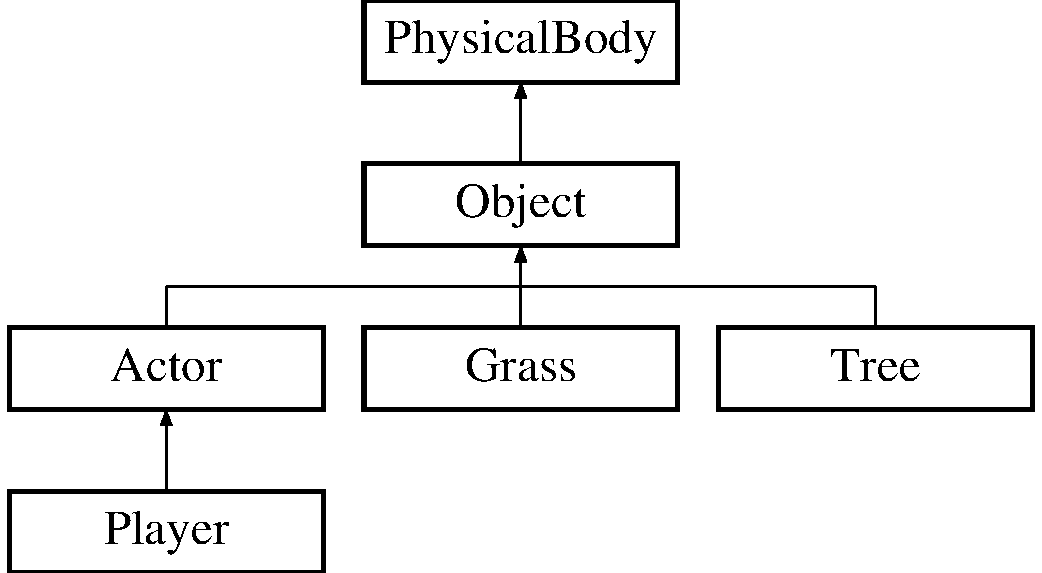
\includegraphics[height=4.000000cm]{classPhysicalBody}
\end{center}
\end{figure}
\subsection*{Public Types}
\begin{DoxyCompactItemize}
\item 
\hypertarget{classPhysicalBody_a11477c65415798a49396b51621e54a70}{}enum {\bfseries Object\+Type} \{ {\bfseries passive} =\textquotesingle{}p\textquotesingle{}, 
{\bfseries dynamic} =\textquotesingle{}d\textquotesingle{}
 \}\label{classPhysicalBody_a11477c65415798a49396b51621e54a70}

\item 
\hypertarget{classPhysicalBody_acfa77263f0e8da678d36bf0a8dde0ed0}{}enum {\bfseries Collision\+Type} \{ {\bfseries ghost} =\textquotesingle{}g\textquotesingle{}, 
{\bfseries solid} =\textquotesingle{}s\textquotesingle{}
 \}\label{classPhysicalBody_acfa77263f0e8da678d36bf0a8dde0ed0}

\item 
\hypertarget{classPhysicalBody_a0242d98735161b0fb3364f21a59eaf41}{}enum {\bfseries Mesh\+Type} \{ {\bfseries circle} =\textquotesingle{}c\textquotesingle{}, 
{\bfseries mesh} =\textquotesingle{}m\textquotesingle{}
 \}\label{classPhysicalBody_a0242d98735161b0fb3364f21a59eaf41}

\end{DoxyCompactItemize}
\subsection*{Public Member Functions}
\begin{DoxyCompactItemize}
\item 
\hyperlink{classPhysicalBody_a32ddf45baf5694a3cc6c405e2ed6e7bf}{Physical\+Body} (Object\+Type type, Collision\+Type collision, \hyperlink{classPointXY}{Point\+X\+Y} dimensions, double friction=1, double mass=1)
\begin{DoxyCompactList}\small\item\em \hyperlink{classPhysicalBody}{Physical\+Body} Constructor without mesh (circle by default) \end{DoxyCompactList}\item 
\hyperlink{classPhysicalBody_ab4285ad124f8e4ed0c9c7fd05fad9268}{Physical\+Body} (Object\+Type type, Collision\+Type collision, \hyperlink{classPointXY}{Point\+X\+Y} dimensions, \hyperlink{classArray}{Array}$<$ \hyperlink{classPointXY}{Point\+X\+Y} $\ast$ $>$ \&collision\+Mesh, double friction=1, double mass=1)
\begin{DoxyCompactList}\small\item\em \hyperlink{classPhysicalBody}{Physical\+Body} Constructor with mesh. \end{DoxyCompactList}\item 
\hyperlink{classPhysicalBody_abfe0f525e4934d83216525a84c9c69f7}{Physical\+Body} (const \hyperlink{classPhysicalBody}{Physical\+Body} \&ref)
\begin{DoxyCompactList}\small\item\em \hyperlink{classPhysicalBody}{Physical\+Body} copy constructor. \end{DoxyCompactList}\item 
const \hyperlink{classPointXY}{Point\+X\+Y} \& \hyperlink{classPhysicalBody_a548eed7049c86fbc46ae96958c8703d7}{get\+Bound} () const 
\begin{DoxyCompactList}\small\item\em get\+Bound returns object bouding box (dimensions) \end{DoxyCompactList}\item 
const \hyperlink{classArray}{Array}$<$ \hyperlink{classVectorXY}{Vector\+X\+Y} $\ast$ $>$ \& \hyperlink{classPhysicalBody_ac2166b0723886ce7f9c040e18ec954c6}{get\+Collision\+Mesh} () const 
\begin{DoxyCompactList}\small\item\em get\+Collision\+Mesh \end{DoxyCompactList}\item 
const \hyperlink{classArray}{Array}$<$ \hyperlink{classVectorXY}{Vector\+X\+Y} $\ast$ $>$ \& \hyperlink{classPhysicalBody_a967028465a40efe44ba6390e3579e210}{get\+Collision\+Normals} () const 
\begin{DoxyCompactList}\small\item\em get\+Collision\+Normals \end{DoxyCompactList}\item 
Object\+Type \hyperlink{classPhysicalBody_a9371f19b3f21435c17ba01b034a01404}{get\+Object\+Type} () const 
\begin{DoxyCompactList}\small\item\em get\+Object\+Type \end{DoxyCompactList}\item 
Collision\+Type \hyperlink{classPhysicalBody_a96d5dba392884dbf83b1f82c621fac9c}{get\+Collision\+Type} () const 
\begin{DoxyCompactList}\small\item\em get\+Collision\+Type \end{DoxyCompactList}\item 
Mesh\+Type \hyperlink{classPhysicalBody_ab6ae355a3cee5918a000220af20f2837}{get\+Mesh\+Type} () const 
\begin{DoxyCompactList}\small\item\em get\+Mesh\+Type \end{DoxyCompactList}\item 
double \hyperlink{classPhysicalBody_af8733082c596676418984ab4c5398f5e}{get\+Friction} () const 
\begin{DoxyCompactList}\small\item\em get\+Friction \end{DoxyCompactList}\item 
double \hyperlink{classPhysicalBody_a8509893e9881d99ed2851338c1be6b55}{get\+Mass} () const 
\begin{DoxyCompactList}\small\item\em get\+Mass \end{DoxyCompactList}\item 
\hypertarget{classPhysicalBody_afef31c3912da9465a1caeed834db6bab}{}void \hyperlink{classPhysicalBody_afef31c3912da9465a1caeed834db6bab}{reshape} ()\label{classPhysicalBody_afef31c3912da9465a1caeed834db6bab}

\begin{DoxyCompactList}\small\item\em reshape strips object collision mesh, turning object into circle type \end{DoxyCompactList}\item 
void \hyperlink{classPhysicalBody_ae7e0ccd04b9e9e83a9777f016b094914}{reshape} (\hyperlink{classArray}{Array}$<$ \hyperlink{classPointXY}{Point\+X\+Y} $\ast$ $>$ \&collision\+Mesh)
\begin{DoxyCompactList}\small\item\em reshape assigns collision mesh polygon to object turning it into mesh (polygon) object type \end{DoxyCompactList}\item 
void \hyperlink{classPhysicalBody_a089a6ea0bbc6e38e9ea09170f123ad64}{set\+Object\+Type} (Object\+Type type)
\begin{DoxyCompactList}\small\item\em set\+Object\+Type \end{DoxyCompactList}\item 
void \hyperlink{classPhysicalBody_ab5aebc5188db718079e4f3e5fc51d8b7}{set\+Collision\+Type} (Collision\+Type collision)
\begin{DoxyCompactList}\small\item\em set\+Collision\+Type \end{DoxyCompactList}\item 
void \hyperlink{classPhysicalBody_a02bfe02d6439f40f41b47ee797533cb6}{set\+Mass} (double mass)
\begin{DoxyCompactList}\small\item\em set\+Mass \end{DoxyCompactList}\item 
void \hyperlink{classPhysicalBody_a44e55add5d12fc288b656f47f983b42a}{set\+Friction} (double friction)
\begin{DoxyCompactList}\small\item\em set\+Friction \end{DoxyCompactList}\item 
\hyperlink{classPhysicalBody}{Physical\+Body} \& \hyperlink{classPhysicalBody_adeff65b6b3f377362e5d3140b8dd9258}{operator=} (const \hyperlink{classPhysicalBody}{Physical\+Body} \&R)
\begin{DoxyCompactList}\small\item\em operator = assignment operator \end{DoxyCompactList}\end{DoxyCompactItemize}
\subsection*{Friends}
\begin{DoxyCompactItemize}
\item 
\hypertarget{classPhysicalBody_a639ae8db08b48373cb96fa3728d3c447}{}class {\bfseries Physics\+Engine}\label{classPhysicalBody_a639ae8db08b48373cb96fa3728d3c447}

\end{DoxyCompactItemize}


\subsection{Detailed Description}
The \hyperlink{classPhysicalBody}{Physical\+Body} class Class providing basic physical capabilities. 

\subsection{Constructor \& Destructor Documentation}
\hypertarget{classPhysicalBody_a32ddf45baf5694a3cc6c405e2ed6e7bf}{}\index{Physical\+Body@{Physical\+Body}!Physical\+Body@{Physical\+Body}}
\index{Physical\+Body@{Physical\+Body}!Physical\+Body@{Physical\+Body}}
\subsubsection[{Physical\+Body}]{\setlength{\rightskip}{0pt plus 5cm}Physical\+Body\+::\+Physical\+Body (
\begin{DoxyParamCaption}
\item[{Object\+Type}]{type, }
\item[{Collision\+Type}]{collision, }
\item[{{\bf Point\+X\+Y}}]{dimensions, }
\item[{double}]{friction = {\ttfamily 1}, }
\item[{double}]{mass = {\ttfamily 1}}
\end{DoxyParamCaption}
)}\label{classPhysicalBody_a32ddf45baf5694a3cc6c405e2ed6e7bf}


\hyperlink{classPhysicalBody}{Physical\+Body} Constructor without mesh (circle by default) 


\begin{DoxyParams}{Parameters}
{\em type} & object type \\
\hline
{\em collision} & collision type \\
\hline
{\em dimensions} & object dimensions as w\+:h pair \\
\hline
{\em friction} & object friction factor \\
\hline
{\em mass} & object mass \\
\hline
\end{DoxyParams}
\hypertarget{classPhysicalBody_ab4285ad124f8e4ed0c9c7fd05fad9268}{}\index{Physical\+Body@{Physical\+Body}!Physical\+Body@{Physical\+Body}}
\index{Physical\+Body@{Physical\+Body}!Physical\+Body@{Physical\+Body}}
\subsubsection[{Physical\+Body}]{\setlength{\rightskip}{0pt plus 5cm}Physical\+Body\+::\+Physical\+Body (
\begin{DoxyParamCaption}
\item[{Object\+Type}]{type, }
\item[{Collision\+Type}]{collision, }
\item[{{\bf Point\+X\+Y}}]{dimensions, }
\item[{{\bf Array}$<$ {\bf Point\+X\+Y} $\ast$ $>$ \&}]{collision\+Mesh, }
\item[{double}]{friction = {\ttfamily 1}, }
\item[{double}]{mass = {\ttfamily 1}}
\end{DoxyParamCaption}
)}\label{classPhysicalBody_ab4285ad124f8e4ed0c9c7fd05fad9268}


\hyperlink{classPhysicalBody}{Physical\+Body} Constructor with mesh. 


\begin{DoxyParams}{Parameters}
{\em type} & object type \\
\hline
{\em collision} & collision type \\
\hline
{\em dimensions} & object dimensions as w\+:h pair \\
\hline
{\em collision\+Mesh} & polygon representing collision mesh provided as set of vertices \\
\hline
{\em friction} & object friction factor \\
\hline
{\em mass} & object mass \\
\hline
\end{DoxyParams}
\hypertarget{classPhysicalBody_abfe0f525e4934d83216525a84c9c69f7}{}\index{Physical\+Body@{Physical\+Body}!Physical\+Body@{Physical\+Body}}
\index{Physical\+Body@{Physical\+Body}!Physical\+Body@{Physical\+Body}}
\subsubsection[{Physical\+Body}]{\setlength{\rightskip}{0pt plus 5cm}Physical\+Body\+::\+Physical\+Body (
\begin{DoxyParamCaption}
\item[{const {\bf Physical\+Body} \&}]{ref}
\end{DoxyParamCaption}
)}\label{classPhysicalBody_abfe0f525e4934d83216525a84c9c69f7}


\hyperlink{classPhysicalBody}{Physical\+Body} copy constructor. 


\begin{DoxyParams}{Parameters}
{\em ref} & reference object \\
\hline
\end{DoxyParams}


\subsection{Member Function Documentation}
\hypertarget{classPhysicalBody_a548eed7049c86fbc46ae96958c8703d7}{}\index{Physical\+Body@{Physical\+Body}!get\+Bound@{get\+Bound}}
\index{get\+Bound@{get\+Bound}!Physical\+Body@{Physical\+Body}}
\subsubsection[{get\+Bound}]{\setlength{\rightskip}{0pt plus 5cm}const {\bf Point\+X\+Y}\& Physical\+Body\+::get\+Bound (
\begin{DoxyParamCaption}
{}
\end{DoxyParamCaption}
) const\hspace{0.3cm}{\ttfamily [inline]}}\label{classPhysicalBody_a548eed7049c86fbc46ae96958c8703d7}


get\+Bound returns object bouding box (dimensions) 

\begin{DoxyReturn}{Returns}
bouding box w\+:h pair 
\end{DoxyReturn}
\hypertarget{classPhysicalBody_ac2166b0723886ce7f9c040e18ec954c6}{}\index{Physical\+Body@{Physical\+Body}!get\+Collision\+Mesh@{get\+Collision\+Mesh}}
\index{get\+Collision\+Mesh@{get\+Collision\+Mesh}!Physical\+Body@{Physical\+Body}}
\subsubsection[{get\+Collision\+Mesh}]{\setlength{\rightskip}{0pt plus 5cm}const {\bf Array}$<${\bf Vector\+X\+Y}$\ast$$>$\& Physical\+Body\+::get\+Collision\+Mesh (
\begin{DoxyParamCaption}
{}
\end{DoxyParamCaption}
) const\hspace{0.3cm}{\ttfamily [inline]}}\label{classPhysicalBody_ac2166b0723886ce7f9c040e18ec954c6}


get\+Collision\+Mesh 

\begin{DoxyReturn}{Returns}
object collision mesh 
\end{DoxyReturn}
\hypertarget{classPhysicalBody_a967028465a40efe44ba6390e3579e210}{}\index{Physical\+Body@{Physical\+Body}!get\+Collision\+Normals@{get\+Collision\+Normals}}
\index{get\+Collision\+Normals@{get\+Collision\+Normals}!Physical\+Body@{Physical\+Body}}
\subsubsection[{get\+Collision\+Normals}]{\setlength{\rightskip}{0pt plus 5cm}const {\bf Array}$<${\bf Vector\+X\+Y}$\ast$$>$\& Physical\+Body\+::get\+Collision\+Normals (
\begin{DoxyParamCaption}
{}
\end{DoxyParamCaption}
) const\hspace{0.3cm}{\ttfamily [inline]}}\label{classPhysicalBody_a967028465a40efe44ba6390e3579e210}


get\+Collision\+Normals 

\begin{DoxyReturn}{Returns}
object normals 
\end{DoxyReturn}
\hypertarget{classPhysicalBody_a96d5dba392884dbf83b1f82c621fac9c}{}\index{Physical\+Body@{Physical\+Body}!get\+Collision\+Type@{get\+Collision\+Type}}
\index{get\+Collision\+Type@{get\+Collision\+Type}!Physical\+Body@{Physical\+Body}}
\subsubsection[{get\+Collision\+Type}]{\setlength{\rightskip}{0pt plus 5cm}Collision\+Type Physical\+Body\+::get\+Collision\+Type (
\begin{DoxyParamCaption}
{}
\end{DoxyParamCaption}
) const\hspace{0.3cm}{\ttfamily [inline]}}\label{classPhysicalBody_a96d5dba392884dbf83b1f82c621fac9c}


get\+Collision\+Type 

\begin{DoxyReturn}{Returns}
object collision type 
\end{DoxyReturn}
\hypertarget{classPhysicalBody_af8733082c596676418984ab4c5398f5e}{}\index{Physical\+Body@{Physical\+Body}!get\+Friction@{get\+Friction}}
\index{get\+Friction@{get\+Friction}!Physical\+Body@{Physical\+Body}}
\subsubsection[{get\+Friction}]{\setlength{\rightskip}{0pt plus 5cm}double Physical\+Body\+::get\+Friction (
\begin{DoxyParamCaption}
{}
\end{DoxyParamCaption}
) const\hspace{0.3cm}{\ttfamily [inline]}}\label{classPhysicalBody_af8733082c596676418984ab4c5398f5e}


get\+Friction 

\begin{DoxyReturn}{Returns}
object friction factor 
\end{DoxyReturn}
\hypertarget{classPhysicalBody_a8509893e9881d99ed2851338c1be6b55}{}\index{Physical\+Body@{Physical\+Body}!get\+Mass@{get\+Mass}}
\index{get\+Mass@{get\+Mass}!Physical\+Body@{Physical\+Body}}
\subsubsection[{get\+Mass}]{\setlength{\rightskip}{0pt plus 5cm}double Physical\+Body\+::get\+Mass (
\begin{DoxyParamCaption}
{}
\end{DoxyParamCaption}
) const\hspace{0.3cm}{\ttfamily [inline]}}\label{classPhysicalBody_a8509893e9881d99ed2851338c1be6b55}


get\+Mass 

\begin{DoxyReturn}{Returns}
object mass 
\end{DoxyReturn}
\hypertarget{classPhysicalBody_ab6ae355a3cee5918a000220af20f2837}{}\index{Physical\+Body@{Physical\+Body}!get\+Mesh\+Type@{get\+Mesh\+Type}}
\index{get\+Mesh\+Type@{get\+Mesh\+Type}!Physical\+Body@{Physical\+Body}}
\subsubsection[{get\+Mesh\+Type}]{\setlength{\rightskip}{0pt plus 5cm}Mesh\+Type Physical\+Body\+::get\+Mesh\+Type (
\begin{DoxyParamCaption}
{}
\end{DoxyParamCaption}
) const\hspace{0.3cm}{\ttfamily [inline]}}\label{classPhysicalBody_ab6ae355a3cee5918a000220af20f2837}


get\+Mesh\+Type 

\begin{DoxyReturn}{Returns}
object mesh type 
\end{DoxyReturn}
\hypertarget{classPhysicalBody_a9371f19b3f21435c17ba01b034a01404}{}\index{Physical\+Body@{Physical\+Body}!get\+Object\+Type@{get\+Object\+Type}}
\index{get\+Object\+Type@{get\+Object\+Type}!Physical\+Body@{Physical\+Body}}
\subsubsection[{get\+Object\+Type}]{\setlength{\rightskip}{0pt plus 5cm}Object\+Type Physical\+Body\+::get\+Object\+Type (
\begin{DoxyParamCaption}
{}
\end{DoxyParamCaption}
) const\hspace{0.3cm}{\ttfamily [inline]}}\label{classPhysicalBody_a9371f19b3f21435c17ba01b034a01404}


get\+Object\+Type 

\begin{DoxyReturn}{Returns}
object type 
\end{DoxyReturn}
\hypertarget{classPhysicalBody_adeff65b6b3f377362e5d3140b8dd9258}{}\index{Physical\+Body@{Physical\+Body}!operator=@{operator=}}
\index{operator=@{operator=}!Physical\+Body@{Physical\+Body}}
\subsubsection[{operator=}]{\setlength{\rightskip}{0pt plus 5cm}{\bf Physical\+Body} \& Physical\+Body\+::operator= (
\begin{DoxyParamCaption}
\item[{const {\bf Physical\+Body} \&}]{R}
\end{DoxyParamCaption}
)}\label{classPhysicalBody_adeff65b6b3f377362e5d3140b8dd9258}


operator = assignment operator 


\begin{DoxyParams}{Parameters}
{\em R} & \\
\hline
\end{DoxyParams}
\begin{DoxyReturn}{Returns}

\end{DoxyReturn}
\hypertarget{classPhysicalBody_ae7e0ccd04b9e9e83a9777f016b094914}{}\index{Physical\+Body@{Physical\+Body}!reshape@{reshape}}
\index{reshape@{reshape}!Physical\+Body@{Physical\+Body}}
\subsubsection[{reshape}]{\setlength{\rightskip}{0pt plus 5cm}void Physical\+Body\+::reshape (
\begin{DoxyParamCaption}
\item[{{\bf Array}$<$ {\bf Point\+X\+Y} $\ast$ $>$ \&}]{collision\+Mesh}
\end{DoxyParamCaption}
)}\label{classPhysicalBody_ae7e0ccd04b9e9e83a9777f016b094914}


reshape assigns collision mesh polygon to object turning it into mesh (polygon) object type 


\begin{DoxyParams}{Parameters}
{\em collision\+Mesh} & \\
\hline
\end{DoxyParams}
\hypertarget{classPhysicalBody_ab5aebc5188db718079e4f3e5fc51d8b7}{}\index{Physical\+Body@{Physical\+Body}!set\+Collision\+Type@{set\+Collision\+Type}}
\index{set\+Collision\+Type@{set\+Collision\+Type}!Physical\+Body@{Physical\+Body}}
\subsubsection[{set\+Collision\+Type}]{\setlength{\rightskip}{0pt plus 5cm}void Physical\+Body\+::set\+Collision\+Type (
\begin{DoxyParamCaption}
\item[{Collision\+Type}]{collision}
\end{DoxyParamCaption}
)\hspace{0.3cm}{\ttfamily [inline]}}\label{classPhysicalBody_ab5aebc5188db718079e4f3e5fc51d8b7}


set\+Collision\+Type 


\begin{DoxyParams}{Parameters}
{\em collision} & new collision type \\
\hline
\end{DoxyParams}
\hypertarget{classPhysicalBody_a44e55add5d12fc288b656f47f983b42a}{}\index{Physical\+Body@{Physical\+Body}!set\+Friction@{set\+Friction}}
\index{set\+Friction@{set\+Friction}!Physical\+Body@{Physical\+Body}}
\subsubsection[{set\+Friction}]{\setlength{\rightskip}{0pt plus 5cm}void Physical\+Body\+::set\+Friction (
\begin{DoxyParamCaption}
\item[{double}]{friction}
\end{DoxyParamCaption}
)\hspace{0.3cm}{\ttfamily [inline]}}\label{classPhysicalBody_a44e55add5d12fc288b656f47f983b42a}


set\+Friction 


\begin{DoxyParams}{Parameters}
{\em friction} & friction factor (can\textquotesingle{}t be negative) \\
\hline
\end{DoxyParams}
\hypertarget{classPhysicalBody_a02bfe02d6439f40f41b47ee797533cb6}{}\index{Physical\+Body@{Physical\+Body}!set\+Mass@{set\+Mass}}
\index{set\+Mass@{set\+Mass}!Physical\+Body@{Physical\+Body}}
\subsubsection[{set\+Mass}]{\setlength{\rightskip}{0pt plus 5cm}void Physical\+Body\+::set\+Mass (
\begin{DoxyParamCaption}
\item[{double}]{mass}
\end{DoxyParamCaption}
)\hspace{0.3cm}{\ttfamily [inline]}}\label{classPhysicalBody_a02bfe02d6439f40f41b47ee797533cb6}


set\+Mass 


\begin{DoxyParams}{Parameters}
{\em mass} & new mass (can\textquotesingle{}t be negative) \\
\hline
\end{DoxyParams}
\hypertarget{classPhysicalBody_a089a6ea0bbc6e38e9ea09170f123ad64}{}\index{Physical\+Body@{Physical\+Body}!set\+Object\+Type@{set\+Object\+Type}}
\index{set\+Object\+Type@{set\+Object\+Type}!Physical\+Body@{Physical\+Body}}
\subsubsection[{set\+Object\+Type}]{\setlength{\rightskip}{0pt plus 5cm}void Physical\+Body\+::set\+Object\+Type (
\begin{DoxyParamCaption}
\item[{Object\+Type}]{type}
\end{DoxyParamCaption}
)\hspace{0.3cm}{\ttfamily [inline]}}\label{classPhysicalBody_a089a6ea0bbc6e38e9ea09170f123ad64}


set\+Object\+Type 


\begin{DoxyParams}{Parameters}
{\em type} & new object type \\
\hline
\end{DoxyParams}


The documentation for this class was generated from the following files\+:\begin{DoxyCompactItemize}
\item 
include/object.\+h\item 
src/object.\+cpp\end{DoxyCompactItemize}

\hypertarget{classPhysicsEngine}{}\section{Physics\+Engine Class Reference}
\label{classPhysicsEngine}\index{Physics\+Engine@{Physics\+Engine}}


The \hyperlink{classPhysicsEngine}{Physics\+Engine} class Class providing basic physics functionality to registered map.  




{\ttfamily \#include $<$physx.\+h$>$}

\subsection*{Classes}
\begin{DoxyCompactItemize}
\item 
class \hyperlink{classPhysicsEngine_1_1CollisionGrid}{Collision\+Grid}
\begin{DoxyCompactList}\small\item\em The \hyperlink{classPhysicsEngine_1_1CollisionGrid}{Collision\+Grid} class Class containing collision grid for optimization purpose. \end{DoxyCompactList}\item 
struct \hyperlink{structPhysicsEngine_1_1CREnt}{C\+R\+Ent}
\end{DoxyCompactItemize}
\subsection*{Public Member Functions}
\begin{DoxyCompactItemize}
\item 
\hyperlink{classPhysicsEngine_abc458126ff199c01fe04bbc910f2190d}{Physics\+Engine} (\hyperlink{classGameMap}{Game\+Map} \&map)
\begin{DoxyCompactList}\small\item\em \hyperlink{classPhysicsEngine}{Physics\+Engine} Constructor. \end{DoxyCompactList}\item 
\hyperlink{classGameMap}{Game\+Map} $\ast$ \hyperlink{classPhysicsEngine_abe9b7fec2565129365490d4d09ab91fb}{get\+Map} () const 
\begin{DoxyCompactList}\small\item\em get\+Map return map registered by engine \end{DoxyCompactList}\item 
\hyperlink{classChain}{Chain}$<$ \hyperlink{structPhysicsEngine_1_1CREnt}{C\+R\+Ent} $>$ $\ast$ \hyperlink{classPhysicsEngine_a52a90ad6bdd5706c6fe89254991330c6}{get\+Collision\+Registry} () const 
\begin{DoxyCompactList}\small\item\em get\+Collision\+Registry returns list of collisions \end{DoxyCompactList}\item 
void \hyperlink{classPhysicsEngine_a37d4d1483678921775e0bc545fc8e0b0}{reload\+Map} (\hyperlink{classGameMap}{Game\+Map} \&map)
\begin{DoxyCompactList}\small\item\em reload\+Map bind engine to different map \end{DoxyCompactList}\item 
void \hyperlink{classPhysicsEngine_ac6d56b0524f4c020463dd6dbbd9dcdc1}{register\+Object} (\hyperlink{classObjectMapMeta}{Object\+Map\+Meta} \&meta)
\begin{DoxyCompactList}\small\item\em register\+Object register object in physics engine \end{DoxyCompactList}\item 
void \hyperlink{classPhysicsEngine_a323e3de1fd9aa734b84fb62a9496f2e2}{unregister\+Object} (\hyperlink{classObjectPhysicsMeta}{Object\+Physics\+Meta} \&meta)
\begin{DoxyCompactList}\small\item\em unregister\+Object unregister object from physics engine \end{DoxyCompactList}\item 
long double \hyperlink{classPhysicsEngine_a71be5c7bd4b8f50a78a3618b57cb0e84}{time\+Shift} ()
\begin{DoxyCompactList}\small\item\em time\+Shift perform physics clock tick \end{DoxyCompactList}\end{DoxyCompactItemize}


\subsection{Detailed Description}
The \hyperlink{classPhysicsEngine}{Physics\+Engine} class Class providing basic physics functionality to registered map. 

\begin{DoxySeeAlso}{See also}
\hyperlink{classGameMap}{Game\+Map} 

\hyperlink{classObjectPhysicsMeta}{Object\+Physics\+Meta} 
\end{DoxySeeAlso}


\subsection{Constructor \& Destructor Documentation}
\hypertarget{classPhysicsEngine_abc458126ff199c01fe04bbc910f2190d}{}\index{Physics\+Engine@{Physics\+Engine}!Physics\+Engine@{Physics\+Engine}}
\index{Physics\+Engine@{Physics\+Engine}!Physics\+Engine@{Physics\+Engine}}
\subsubsection[{Physics\+Engine}]{\setlength{\rightskip}{0pt plus 5cm}Physics\+Engine\+::\+Physics\+Engine (
\begin{DoxyParamCaption}
\item[{{\bf Game\+Map} \&}]{map}
\end{DoxyParamCaption}
)}\label{classPhysicsEngine_abc458126ff199c01fe04bbc910f2190d}


\hyperlink{classPhysicsEngine}{Physics\+Engine} Constructor. 


\begin{DoxyParams}{Parameters}
{\em map} & map to register physics engine for \\
\hline
\end{DoxyParams}


\subsection{Member Function Documentation}
\hypertarget{classPhysicsEngine_a52a90ad6bdd5706c6fe89254991330c6}{}\index{Physics\+Engine@{Physics\+Engine}!get\+Collision\+Registry@{get\+Collision\+Registry}}
\index{get\+Collision\+Registry@{get\+Collision\+Registry}!Physics\+Engine@{Physics\+Engine}}
\subsubsection[{get\+Collision\+Registry}]{\setlength{\rightskip}{0pt plus 5cm}{\bf Chain}$<${\bf C\+R\+Ent}$>$$\ast$ Physics\+Engine\+::get\+Collision\+Registry (
\begin{DoxyParamCaption}
{}
\end{DoxyParamCaption}
) const\hspace{0.3cm}{\ttfamily [inline]}}\label{classPhysicsEngine_a52a90ad6bdd5706c6fe89254991330c6}


get\+Collision\+Registry returns list of collisions 

\begin{DoxyReturn}{Returns}
list of collisions 
\end{DoxyReturn}
\hypertarget{classPhysicsEngine_abe9b7fec2565129365490d4d09ab91fb}{}\index{Physics\+Engine@{Physics\+Engine}!get\+Map@{get\+Map}}
\index{get\+Map@{get\+Map}!Physics\+Engine@{Physics\+Engine}}
\subsubsection[{get\+Map}]{\setlength{\rightskip}{0pt plus 5cm}{\bf Game\+Map}$\ast$ Physics\+Engine\+::get\+Map (
\begin{DoxyParamCaption}
{}
\end{DoxyParamCaption}
) const\hspace{0.3cm}{\ttfamily [inline]}}\label{classPhysicsEngine_abe9b7fec2565129365490d4d09ab91fb}


get\+Map return map registered by engine 

\begin{DoxyReturn}{Returns}
map registered by engine 
\end{DoxyReturn}
\hypertarget{classPhysicsEngine_ac6d56b0524f4c020463dd6dbbd9dcdc1}{}\index{Physics\+Engine@{Physics\+Engine}!register\+Object@{register\+Object}}
\index{register\+Object@{register\+Object}!Physics\+Engine@{Physics\+Engine}}
\subsubsection[{register\+Object}]{\setlength{\rightskip}{0pt plus 5cm}void Physics\+Engine\+::register\+Object (
\begin{DoxyParamCaption}
\item[{{\bf Object\+Map\+Meta} \&}]{meta}
\end{DoxyParamCaption}
)}\label{classPhysicsEngine_ac6d56b0524f4c020463dd6dbbd9dcdc1}


register\+Object register object in physics engine 


\begin{DoxyParams}{Parameters}
{\em meta} & meta to be registered \\
\hline
\end{DoxyParams}
\hypertarget{classPhysicsEngine_a37d4d1483678921775e0bc545fc8e0b0}{}\index{Physics\+Engine@{Physics\+Engine}!reload\+Map@{reload\+Map}}
\index{reload\+Map@{reload\+Map}!Physics\+Engine@{Physics\+Engine}}
\subsubsection[{reload\+Map}]{\setlength{\rightskip}{0pt plus 5cm}void Physics\+Engine\+::reload\+Map (
\begin{DoxyParamCaption}
\item[{{\bf Game\+Map} \&}]{map}
\end{DoxyParamCaption}
)}\label{classPhysicsEngine_a37d4d1483678921775e0bc545fc8e0b0}


reload\+Map bind engine to different map 


\begin{DoxyParams}{Parameters}
{\em map} & new map to be bound to \\
\hline
\end{DoxyParams}
\hypertarget{classPhysicsEngine_a71be5c7bd4b8f50a78a3618b57cb0e84}{}\index{Physics\+Engine@{Physics\+Engine}!time\+Shift@{time\+Shift}}
\index{time\+Shift@{time\+Shift}!Physics\+Engine@{Physics\+Engine}}
\subsubsection[{time\+Shift}]{\setlength{\rightskip}{0pt plus 5cm}long double Physics\+Engine\+::time\+Shift (
\begin{DoxyParamCaption}
{}
\end{DoxyParamCaption}
)}\label{classPhysicsEngine_a71be5c7bd4b8f50a78a3618b57cb0e84}


time\+Shift perform physics clock tick 

\begin{DoxyReturn}{Returns}
time shifted by engine 
\end{DoxyReturn}
\hypertarget{classPhysicsEngine_a323e3de1fd9aa734b84fb62a9496f2e2}{}\index{Physics\+Engine@{Physics\+Engine}!unregister\+Object@{unregister\+Object}}
\index{unregister\+Object@{unregister\+Object}!Physics\+Engine@{Physics\+Engine}}
\subsubsection[{unregister\+Object}]{\setlength{\rightskip}{0pt plus 5cm}void Physics\+Engine\+::unregister\+Object (
\begin{DoxyParamCaption}
\item[{{\bf Object\+Physics\+Meta} \&}]{meta}
\end{DoxyParamCaption}
)}\label{classPhysicsEngine_a323e3de1fd9aa734b84fb62a9496f2e2}


unregister\+Object unregister object from physics engine 


\begin{DoxyParams}{Parameters}
{\em meta} & meta to be unregistered \\
\hline
\end{DoxyParams}


The documentation for this class was generated from the following files\+:\begin{DoxyCompactItemize}
\item 
include/physx.\+h\item 
src/physx.\+cpp\end{DoxyCompactItemize}

\hypertarget{classPlayer}{}\section{Player Class Reference}
\label{classPlayer}\index{Player@{Player}}


The \hyperlink{classPlayer}{Player} Class is a expanded version of \hyperlink{classActor}{Actor} class.  




{\ttfamily \#include $<$Actor.\+h$>$}

Inheritance diagram for Player\+:\begin{figure}[H]
\begin{center}
\leavevmode
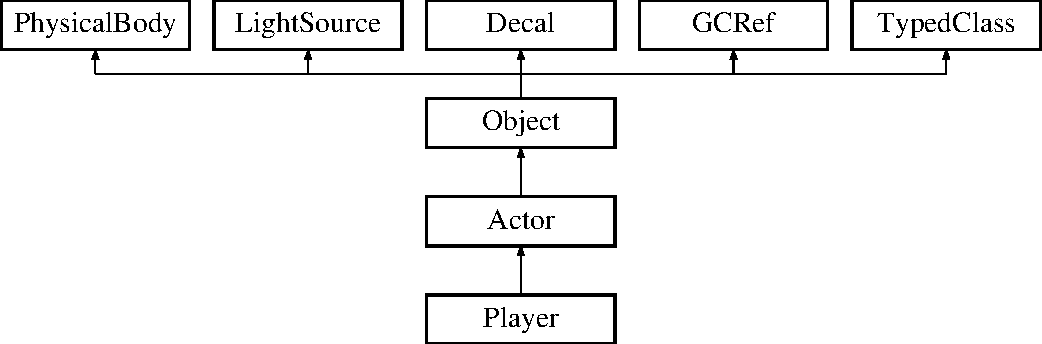
\includegraphics[height=4.000000cm]{classPlayer}
\end{center}
\end{figure}
\subsection*{Public Member Functions}
\begin{DoxyCompactItemize}
\item 
\hypertarget{classPlayer_ae7423d709bb8ce4bd3c0a2abf6acfba0}{}{\bfseries Player} (std\+::string N=\char`\"{}Player\char`\"{}, float maxhp=1, float curhp=1, int lvl=1)\label{classPlayer_ae7423d709bb8ce4bd3c0a2abf6acfba0}

\item 
\hypertarget{classPlayer_a832c45eb6c4c3b7a85098eea14bff5c1}{}float \hyperlink{classPlayer_a832c45eb6c4c3b7a85098eea14bff5c1}{get\+Gained\+Experience} () const \label{classPlayer_a832c45eb6c4c3b7a85098eea14bff5c1}

\begin{DoxyCompactList}\small\item\em Thanks to that we can check what is in class variable Gained\+Experience. \end{DoxyCompactList}\item 
\hypertarget{classPlayer_a87007e274e6588713352a3836e6411a2}{}float \hyperlink{classPlayer_a87007e274e6588713352a3836e6411a2}{get\+To\+Next\+Level\+Experience} () const \label{classPlayer_a87007e274e6588713352a3836e6411a2}

\begin{DoxyCompactList}\small\item\em Thanks to that we can check what is in class variable To\+Next\+Level\+Experience. \end{DoxyCompactList}\item 
\hypertarget{classPlayer_a8b2c3f2f4e2247e2fb394c6868781d9b}{}void \hyperlink{classPlayer_a8b2c3f2f4e2247e2fb394c6868781d9b}{Add\+Experience} (float exp)\label{classPlayer_a8b2c3f2f4e2247e2fb394c6868781d9b}

\begin{DoxyCompactList}\small\item\em We can add experience to current experience. \end{DoxyCompactList}\item 
\hypertarget{classPlayer_aae180f7a4a011ba1fd485e3d8728f489}{}void \hyperlink{classPlayer_aae180f7a4a011ba1fd485e3d8728f489}{Level\+Up} ()\label{classPlayer_aae180f7a4a011ba1fd485e3d8728f489}

\begin{DoxyCompactList}\small\item\em Add one to class variable Level. \end{DoxyCompactList}\end{DoxyCompactItemize}
\subsection*{Static Public Attributes}
\begin{DoxyCompactItemize}
\item 
\hypertarget{classPlayer_a0b125b1e2117688adffc2e89db2fb53a}{}static constexpr char $\ast$ {\bfseries type\+Name} =(char$\ast$)\char`\"{}Player\char`\"{}\label{classPlayer_a0b125b1e2117688adffc2e89db2fb53a}

\end{DoxyCompactItemize}
\subsection*{Additional Inherited Members}


\subsection{Detailed Description}
The \hyperlink{classPlayer}{Player} Class is a expanded version of \hyperlink{classActor}{Actor} class. 

Class contain some extra attributes which helped player in game;

\begin{DoxySeeAlso}{See also}
\hyperlink{classObject}{Object} 

\hyperlink{classActor}{Actor} 
\end{DoxySeeAlso}


The documentation for this class was generated from the following files\+:\begin{DoxyCompactItemize}
\item 
drivers/include/Actor.\+h\item 
drivers/src/Actor.\+cpp\end{DoxyCompactItemize}

\hypertarget{classPlayerController}{}\section{Player\+Controller Class Reference}
\label{classPlayerController}\index{Player\+Controller@{Player\+Controller}}


The \hyperlink{classPlayerController}{Player\+Controller} Class is a tool which we add to session and this allow us to control a \hyperlink{classPlayer}{Player} \hyperlink{classObject}{Object} in game.  




{\ttfamily \#include $<$Player\+Controller.\+h$>$}

Inheritance diagram for Player\+Controller\+:\begin{figure}[H]
\begin{center}
\leavevmode
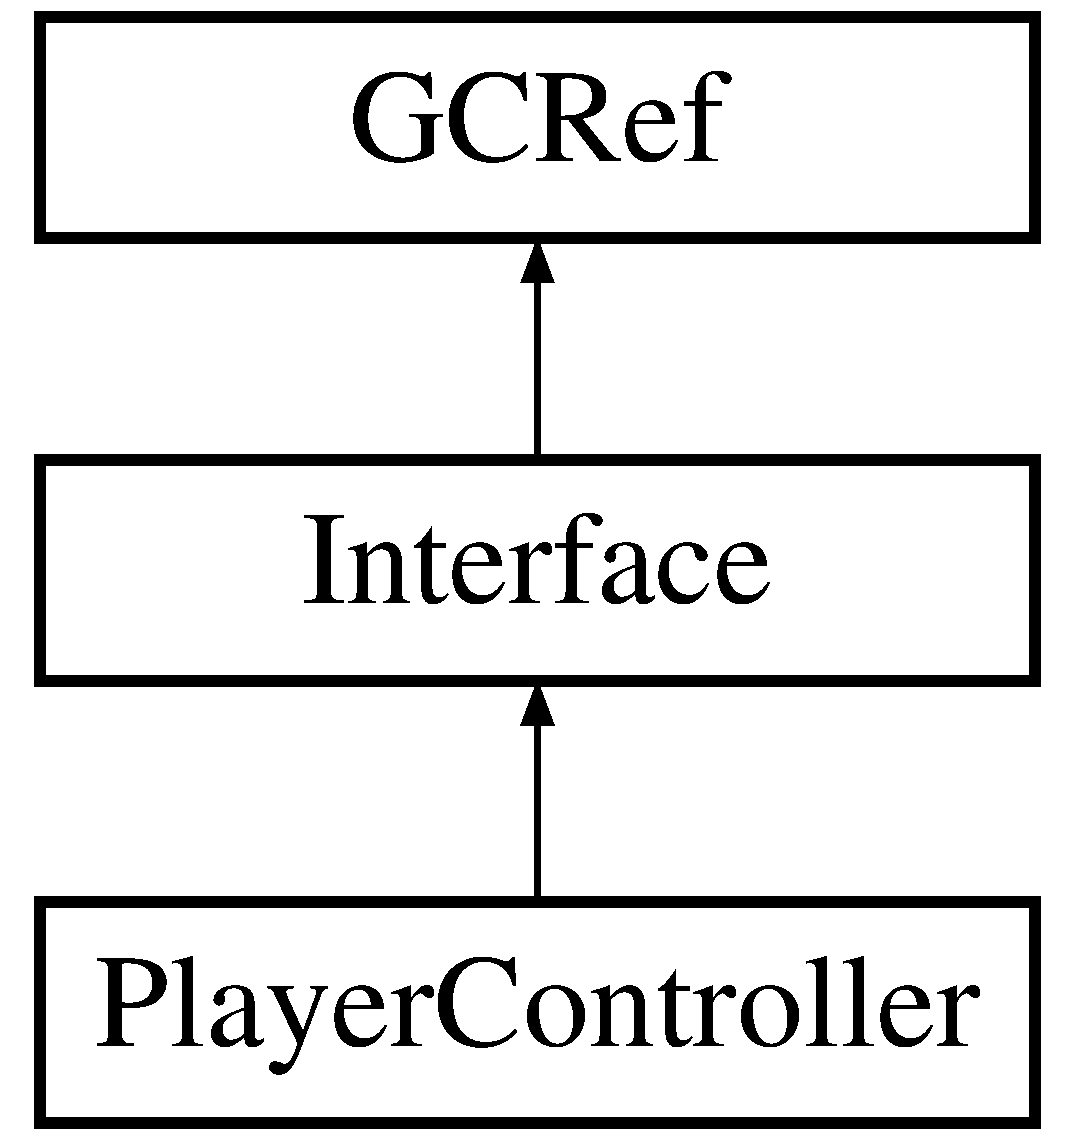
\includegraphics[height=3.000000cm]{classPlayerController}
\end{center}
\end{figure}
\subsection*{Public Member Functions}
\begin{DoxyCompactItemize}
\item 
void \hyperlink{classPlayerController_a1d348ae7dbf9730dde7b6c76e27b2d4b}{set\+Player\+Holder} (\hyperlink{classObjectMapMeta}{Object\+Map\+Meta} $\ast$M\+M)
\begin{DoxyCompactList}\small\item\em Setting a class variable set\+Player\+Holder. \end{DoxyCompactList}\item 
\hypertarget{classPlayerController_a062dc3debb7d14f2fc755b1b44ae7d07}{}\hyperlink{classBaseEvent}{Base\+Event} \& \hyperlink{classPlayerController_a062dc3debb7d14f2fc755b1b44ae7d07}{run} (\hyperlink{classGameSession}{Game\+Session} \&session)\label{classPlayerController_a062dc3debb7d14f2fc755b1b44ae7d07}

\begin{DoxyCompactList}\small\item\em Basic funtion which control a session. \end{DoxyCompactList}\end{DoxyCompactItemize}


\subsection{Detailed Description}
The \hyperlink{classPlayerController}{Player\+Controller} Class is a tool which we add to session and this allow us to control a \hyperlink{classPlayer}{Player} \hyperlink{classObject}{Object} in game. 

\begin{DoxySeeAlso}{See also}
\hyperlink{classInterface}{Interface} 
\end{DoxySeeAlso}


\subsection{Member Function Documentation}
\hypertarget{classPlayerController_a1d348ae7dbf9730dde7b6c76e27b2d4b}{}\index{Player\+Controller@{Player\+Controller}!set\+Player\+Holder@{set\+Player\+Holder}}
\index{set\+Player\+Holder@{set\+Player\+Holder}!Player\+Controller@{Player\+Controller}}
\subsubsection[{set\+Player\+Holder}]{\setlength{\rightskip}{0pt plus 5cm}void Player\+Controller\+::set\+Player\+Holder (
\begin{DoxyParamCaption}
\item[{{\bf Object\+Map\+Meta} $\ast$}]{M\+M}
\end{DoxyParamCaption}
)}\label{classPlayerController_a1d348ae7dbf9730dde7b6c76e27b2d4b}


Setting a class variable set\+Player\+Holder. 



The documentation for this class was generated from the following files\+:\begin{DoxyCompactItemize}
\item 
drivers/include/Player\+Controller.\+h\item 
drivers/src/Player\+Controller.\+cpp\end{DoxyCompactItemize}

\hypertarget{classPointXY}{}\section{Point\+X\+Y Class Reference}
\label{classPointXY}\index{Point\+X\+Y@{Point\+X\+Y}}


The \hyperlink{classPointXY}{Point\+X\+Y} class class providing basic point functionality.  




{\ttfamily \#include $<$Point\+X\+Y.\+h$>$}

\subsection*{Public Member Functions}
\begin{DoxyCompactItemize}
\item 
\hyperlink{classPointXY_aab6d5e59dcd1183ce1fefb62a0620ed5}{Point\+X\+Y} (long double \hyperlink{classPointXY_a134e66580fce7d7c4c7f0a6fb80f3040}{X}=0, long double \hyperlink{classPointXY_a9e1a37c00a0fec942609fcd9185d1a10}{Y}=0)
\begin{DoxyCompactList}\small\item\em \hyperlink{classPointXY}{Point\+X\+Y} basic constructor. \end{DoxyCompactList}\item 
\hyperlink{classPointXY_a04df1b6e01e5521a7ad28aa8e5b3e830}{Point\+X\+Y} (const \hyperlink{classPointXY}{Point\+X\+Y} \&tmp)
\begin{DoxyCompactList}\small\item\em \hyperlink{classPointXY}{Point\+X\+Y} copy constructor. \end{DoxyCompactList}\item 
void \hyperlink{classPointXY_a696701ac3b43657e94284244f21f20f6}{change\+To} (long double \hyperlink{classPointXY_a134e66580fce7d7c4c7f0a6fb80f3040}{X}, long double \hyperlink{classPointXY_a9e1a37c00a0fec942609fcd9185d1a10}{Y})
\begin{DoxyCompactList}\small\item\em change\+To change point parameters \end{DoxyCompactList}\item 
void \hyperlink{classPointXY_a6bdc68a97ba4556cdefa9cff3f22089b}{change\+To} (const \hyperlink{classPointXY}{Point\+X\+Y} \&tmp)
\begin{DoxyCompactList}\small\item\em change\+To copy parameters from other point to this one \end{DoxyCompactList}\item 
void \hyperlink{classPointXY_a2be0c9202aaa1963faa32f84ba8f5573}{move\+By} (long double \hyperlink{classPointXY_a134e66580fce7d7c4c7f0a6fb80f3040}{X}, long double \hyperlink{classPointXY_a9e1a37c00a0fec942609fcd9185d1a10}{Y})
\begin{DoxyCompactList}\small\item\em move\+By move point by specified offset \end{DoxyCompactList}\item 
void \hyperlink{classPointXY_a8a020ce7e0ea6b7b694555d21d8e780c}{move\+By} (const \hyperlink{classPointXY}{Point\+X\+Y} \&tmp)
\begin{DoxyCompactList}\small\item\em move\+By move point by offset specified as point \end{DoxyCompactList}\item 
long double \hyperlink{classPointXY_ad0a3960b3701e91d54ff2533c5b69809}{get\+X} () const 
\begin{DoxyCompactList}\small\item\em get\+X return x coordinate \end{DoxyCompactList}\item 
long double \hyperlink{classPointXY_ad0d22647ef668ea39a630bac5bb1c046}{get\+Y} () const 
\begin{DoxyCompactList}\small\item\em get\+Y return y coordinate \end{DoxyCompactList}\item 
\hypertarget{classPointXY_ab543f519c25866bd1c9d04c093d20478}{}\hyperlink{classPointXY}{Point\+X\+Y} {\bfseries operator+} (const \hyperlink{classPointXY}{Point\+X\+Y} point) const \label{classPointXY_ab543f519c25866bd1c9d04c093d20478}

\item 
\hypertarget{classPointXY_a7b138c1896e62a8f920ed4f797b3cbfe}{}\hyperlink{classPointXY}{Point\+X\+Y} {\bfseries operator-\/} (const \hyperlink{classPointXY}{Point\+X\+Y} point) const \label{classPointXY_a7b138c1896e62a8f920ed4f797b3cbfe}

\item 
\hypertarget{classPointXY_ab126ab992e6fbeff7c39487fa94a8827}{}void {\bfseries operator+=} (const \hyperlink{classPointXY}{Point\+X\+Y} point)\label{classPointXY_ab126ab992e6fbeff7c39487fa94a8827}

\item 
\hypertarget{classPointXY_aadf351c6944336e734950093d031cc5a}{}void {\bfseries operator-\/=} (const \hyperlink{classPointXY}{Point\+X\+Y} point)\label{classPointXY_aadf351c6944336e734950093d031cc5a}

\item 
\hypertarget{classPointXY_a6ce939a48ba2f22460762da7c79e86c5}{}\hyperlink{classPointXY}{Point\+X\+Y} {\bfseries operator$\ast$} (double k) const \label{classPointXY_a6ce939a48ba2f22460762da7c79e86c5}

\item 
\hypertarget{classPointXY_a5df03dbc2757ffe8c5db61cfabb24f20}{}void {\bfseries operator$\ast$=} (double k)\label{classPointXY_a5df03dbc2757ffe8c5db61cfabb24f20}

\item 
\hypertarget{classPointXY_a51f8be09d28e4f060205f96fb3e82ff9}{}bool {\bfseries operator==} (const \hyperlink{classPointXY}{Point\+X\+Y} \&point) const \label{classPointXY_a51f8be09d28e4f060205f96fb3e82ff9}

\item 
\hypertarget{classPointXY_adfd80277c5f774c724426205007e87df}{}bool {\bfseries operator!=} (const \hyperlink{classPointXY}{Point\+X\+Y} \&point) const \label{classPointXY_adfd80277c5f774c724426205007e87df}

\end{DoxyCompactItemize}
\subsection*{Public Attributes}
\begin{DoxyCompactItemize}
\item 
\hypertarget{classPointXY_a134e66580fce7d7c4c7f0a6fb80f3040}{}long double \hyperlink{classPointXY_a134e66580fce7d7c4c7f0a6fb80f3040}{X}\label{classPointXY_a134e66580fce7d7c4c7f0a6fb80f3040}

\begin{DoxyCompactList}\small\item\em point x \end{DoxyCompactList}\item 
\hypertarget{classPointXY_a9e1a37c00a0fec942609fcd9185d1a10}{}long double \hyperlink{classPointXY_a9e1a37c00a0fec942609fcd9185d1a10}{Y}\label{classPointXY_a9e1a37c00a0fec942609fcd9185d1a10}

\begin{DoxyCompactList}\small\item\em point y \end{DoxyCompactList}\end{DoxyCompactItemize}
\subsection*{Friends}
\begin{DoxyCompactItemize}
\item 
\hypertarget{classPointXY_a5f925e3bd89f64d9565b4591988c9bdf}{}\hyperlink{classPointXY}{Point\+X\+Y} {\bfseries operator$\ast$} (const double \&k, const \hyperlink{classPointXY}{Point\+X\+Y} \&point)\label{classPointXY_a5f925e3bd89f64d9565b4591988c9bdf}

\end{DoxyCompactItemize}


\subsection{Detailed Description}
The \hyperlink{classPointXY}{Point\+X\+Y} class class providing basic point functionality. 

Can be used as pair of numbers as well 

\subsection{Constructor \& Destructor Documentation}
\hypertarget{classPointXY_aab6d5e59dcd1183ce1fefb62a0620ed5}{}\index{Point\+X\+Y@{Point\+X\+Y}!Point\+X\+Y@{Point\+X\+Y}}
\index{Point\+X\+Y@{Point\+X\+Y}!Point\+X\+Y@{Point\+X\+Y}}
\subsubsection[{Point\+X\+Y}]{\setlength{\rightskip}{0pt plus 5cm}Point\+X\+Y\+::\+Point\+X\+Y (
\begin{DoxyParamCaption}
\item[{long double}]{X = {\ttfamily 0}, }
\item[{long double}]{Y = {\ttfamily 0}}
\end{DoxyParamCaption}
)}\label{classPointXY_aab6d5e59dcd1183ce1fefb62a0620ed5}


\hyperlink{classPointXY}{Point\+X\+Y} basic constructor. 


\begin{DoxyParams}{Parameters}
{\em X} & x \\
\hline
{\em Y} & y \\
\hline
\end{DoxyParams}
\hypertarget{classPointXY_a04df1b6e01e5521a7ad28aa8e5b3e830}{}\index{Point\+X\+Y@{Point\+X\+Y}!Point\+X\+Y@{Point\+X\+Y}}
\index{Point\+X\+Y@{Point\+X\+Y}!Point\+X\+Y@{Point\+X\+Y}}
\subsubsection[{Point\+X\+Y}]{\setlength{\rightskip}{0pt plus 5cm}Point\+X\+Y\+::\+Point\+X\+Y (
\begin{DoxyParamCaption}
\item[{const {\bf Point\+X\+Y} \&}]{tmp}
\end{DoxyParamCaption}
)}\label{classPointXY_a04df1b6e01e5521a7ad28aa8e5b3e830}


\hyperlink{classPointXY}{Point\+X\+Y} copy constructor. 


\begin{DoxyParams}{Parameters}
{\em tmp} & \\
\hline
\end{DoxyParams}


\subsection{Member Function Documentation}
\hypertarget{classPointXY_a696701ac3b43657e94284244f21f20f6}{}\index{Point\+X\+Y@{Point\+X\+Y}!change\+To@{change\+To}}
\index{change\+To@{change\+To}!Point\+X\+Y@{Point\+X\+Y}}
\subsubsection[{change\+To}]{\setlength{\rightskip}{0pt plus 5cm}void Point\+X\+Y\+::change\+To (
\begin{DoxyParamCaption}
\item[{long double}]{X, }
\item[{long double}]{Y}
\end{DoxyParamCaption}
)}\label{classPointXY_a696701ac3b43657e94284244f21f20f6}


change\+To change point parameters 


\begin{DoxyParams}{Parameters}
{\em X} & \\
\hline
{\em Y} & \\
\hline
\end{DoxyParams}
\hypertarget{classPointXY_a6bdc68a97ba4556cdefa9cff3f22089b}{}\index{Point\+X\+Y@{Point\+X\+Y}!change\+To@{change\+To}}
\index{change\+To@{change\+To}!Point\+X\+Y@{Point\+X\+Y}}
\subsubsection[{change\+To}]{\setlength{\rightskip}{0pt plus 5cm}void Point\+X\+Y\+::change\+To (
\begin{DoxyParamCaption}
\item[{const {\bf Point\+X\+Y} \&}]{tmp}
\end{DoxyParamCaption}
)}\label{classPointXY_a6bdc68a97ba4556cdefa9cff3f22089b}


change\+To copy parameters from other point to this one 


\begin{DoxyParams}{Parameters}
{\em tmp} & reference point \\
\hline
\end{DoxyParams}
\hypertarget{classPointXY_ad0a3960b3701e91d54ff2533c5b69809}{}\index{Point\+X\+Y@{Point\+X\+Y}!get\+X@{get\+X}}
\index{get\+X@{get\+X}!Point\+X\+Y@{Point\+X\+Y}}
\subsubsection[{get\+X}]{\setlength{\rightskip}{0pt plus 5cm}long double Point\+X\+Y\+::get\+X (
\begin{DoxyParamCaption}
{}
\end{DoxyParamCaption}
) const\hspace{0.3cm}{\ttfamily [inline]}}\label{classPointXY_ad0a3960b3701e91d54ff2533c5b69809}


get\+X return x coordinate 

\begin{DoxyReturn}{Returns}
x pos 
\end{DoxyReturn}
\hypertarget{classPointXY_ad0d22647ef668ea39a630bac5bb1c046}{}\index{Point\+X\+Y@{Point\+X\+Y}!get\+Y@{get\+Y}}
\index{get\+Y@{get\+Y}!Point\+X\+Y@{Point\+X\+Y}}
\subsubsection[{get\+Y}]{\setlength{\rightskip}{0pt plus 5cm}long double Point\+X\+Y\+::get\+Y (
\begin{DoxyParamCaption}
{}
\end{DoxyParamCaption}
) const\hspace{0.3cm}{\ttfamily [inline]}}\label{classPointXY_ad0d22647ef668ea39a630bac5bb1c046}


get\+Y return y coordinate 

\begin{DoxyReturn}{Returns}
y pos 
\end{DoxyReturn}
\hypertarget{classPointXY_a2be0c9202aaa1963faa32f84ba8f5573}{}\index{Point\+X\+Y@{Point\+X\+Y}!move\+By@{move\+By}}
\index{move\+By@{move\+By}!Point\+X\+Y@{Point\+X\+Y}}
\subsubsection[{move\+By}]{\setlength{\rightskip}{0pt plus 5cm}void Point\+X\+Y\+::move\+By (
\begin{DoxyParamCaption}
\item[{long double}]{X, }
\item[{long double}]{Y}
\end{DoxyParamCaption}
)}\label{classPointXY_a2be0c9202aaa1963faa32f84ba8f5573}


move\+By move point by specified offset 


\begin{DoxyParams}{Parameters}
{\em X} & x offset \\
\hline
{\em Y} & y offset \\
\hline
\end{DoxyParams}
\hypertarget{classPointXY_a8a020ce7e0ea6b7b694555d21d8e780c}{}\index{Point\+X\+Y@{Point\+X\+Y}!move\+By@{move\+By}}
\index{move\+By@{move\+By}!Point\+X\+Y@{Point\+X\+Y}}
\subsubsection[{move\+By}]{\setlength{\rightskip}{0pt plus 5cm}void Point\+X\+Y\+::move\+By (
\begin{DoxyParamCaption}
\item[{const {\bf Point\+X\+Y} \&}]{tmp}
\end{DoxyParamCaption}
)}\label{classPointXY_a8a020ce7e0ea6b7b694555d21d8e780c}


move\+By move point by offset specified as point 


\begin{DoxyParams}{Parameters}
{\em tmp} & \\
\hline
\end{DoxyParams}


The documentation for this class was generated from the following files\+:\begin{DoxyCompactItemize}
\item 
include/Point\+X\+Y.\+h\item 
src/Point\+X\+Y.\+cpp\end{DoxyCompactItemize}

\hypertarget{classRenderEngine}{}\section{Render\+Engine Class Reference}
\label{classRenderEngine}\index{Render\+Engine@{Render\+Engine}}


The \hyperlink{classRenderEngine}{Render\+Engine} class rendering engine for game.  




{\ttfamily \#include $<$gfx.\+h$>$}

\subsection*{Classes}
\begin{DoxyCompactItemize}
\item 
struct \hyperlink{structRenderEngine_1_1objRecord}{obj\+Record}
\end{DoxyCompactItemize}
\subsection*{Public Member Functions}
\begin{DoxyCompactItemize}
\item 
\hyperlink{classRenderEngine_a31ae68425b2e62e0e1f427fe7e2c1a75}{Render\+Engine} (int obj\+Buffer\+Size=\hyperlink{classRenderEngine_a9dc4537015d6db0e13cf78364caacddf}{Render\+Engine\+::default\+Buffer\+Size}, bool autoresize=false, bool resizeable=true, const char $\ast$title=Render\+Engine\+::default\+Window\+Name)
\begin{DoxyCompactList}\small\item\em \hyperlink{classRenderEngine}{Render\+Engine} basic constructor. \end{DoxyCompactList}\item 
\hypertarget{classRenderEngine_a310e9e1d0a3f9bf46e8fe37b0acea878}{}{\bfseries Render\+Engine} (bool autoresize, bool resizeable=true, const char $\ast$title=Render\+Engine\+::default\+Window\+Name)\label{classRenderEngine_a310e9e1d0a3f9bf46e8fe37b0acea878}

\item 
void \hyperlink{classRenderEngine_ae737efb1b6933f10aa12b991a3deb1fa}{push\+Object} (const \hyperlink{classPointXY}{Point\+X\+Y} position, const \hyperlink{classDecal}{Decal} \&decal)
\begin{DoxyCompactList}\small\item\em push\+Object add new \hyperlink{classDecal}{Decal} to render queue \end{DoxyCompactList}\item 
\hypertarget{classRenderEngine_ab09f2455f3da1dddc07b478405f8f01b}{}void \hyperlink{classRenderEngine_ab09f2455f3da1dddc07b478405f8f01b}{clear} ()\label{classRenderEngine_ab09f2455f3da1dddc07b478405f8f01b}

\begin{DoxyCompactList}\small\item\em clear clear draw buffer \end{DoxyCompactList}\item 
\hypertarget{classRenderEngine_a4e56228f0972018bc593e5d62da83f1d}{}void \hyperlink{classRenderEngine_a4e56228f0972018bc593e5d62da83f1d}{flush} ()\label{classRenderEngine_a4e56228f0972018bc593e5d62da83f1d}

\begin{DoxyCompactList}\small\item\em flush flush draw buffer \end{DoxyCompactList}\item 
void \hyperlink{classRenderEngine_a99306b968abe7132a853513e9b2046b2}{center\+Camera} (const \hyperlink{classPointXY}{Point\+X\+Y} pos)
\begin{DoxyCompactList}\small\item\em center\+Camera center camera on specified point \end{DoxyCompactList}\item 
\hypertarget{classRenderEngine_ab146273934ea5d1b3f76dd21c456570c}{}void {\bfseries center\+Camera} (int W, int H)\label{classRenderEngine_ab146273934ea5d1b3f76dd21c456570c}

\item 
void \hyperlink{classRenderEngine_a6b3570ba21bac9e92bd2caebc8362b16}{canvas\+Resize} (const \hyperlink{classPointXY}{Point\+X\+Y} size)
\begin{DoxyCompactList}\small\item\em canvas\+Resize resize virtual canvas \end{DoxyCompactList}\item 
\hypertarget{classRenderEngine_a9ed2b4db51b92a361ec13c1c5be51ce5}{}void {\bfseries canvas\+Resize} (int W, int H)\label{classRenderEngine_a9ed2b4db51b92a361ec13c1c5be51ce5}

\item 
void \hyperlink{classRenderEngine_a92afa48be7f48d9e5697fbb878348267}{resize\+Draw\+Buffer} (int max\+Obj\+Count)
\begin{DoxyCompactList}\small\item\em resize\+Draw\+Buffer resize draw buffer \end{DoxyCompactList}\item 
void \hyperlink{classRenderEngine_a78ce63c93988c74ec7b5d5535570c001}{set\+Window\+Title} (const char $\ast$title)
\begin{DoxyCompactList}\small\item\em set\+Window\+Title set window title \end{DoxyCompactList}\end{DoxyCompactItemize}
\subsection*{Static Public Attributes}
\begin{DoxyCompactItemize}
\item 
\hypertarget{classRenderEngine_a6e727b66ab4af5ec0a3db0020217137c}{}static constexpr int \hyperlink{classRenderEngine_a6e727b66ab4af5ec0a3db0020217137c}{U\+N\+I\+T\+S\+I\+Z\+E} =10\label{classRenderEngine_a6e727b66ab4af5ec0a3db0020217137c}

\begin{DoxyCompactList}\small\item\em size of single session-\/wise unit in px \end{DoxyCompactList}\item 
\hypertarget{classRenderEngine_a9dc4537015d6db0e13cf78364caacddf}{}static constexpr int \hyperlink{classRenderEngine_a9dc4537015d6db0e13cf78364caacddf}{default\+Buffer\+Size} =256\label{classRenderEngine_a9dc4537015d6db0e13cf78364caacddf}

\begin{DoxyCompactList}\small\item\em default draw buffer size \end{DoxyCompactList}\item 
\hypertarget{classRenderEngine_a2039eceae60c84d8640e01cf76dd7e06}{}static constexpr char $\ast$ {\bfseries default\+Window\+Name} =(char$\ast$)\char`\"{}Game window\char`\"{}\label{classRenderEngine_a2039eceae60c84d8640e01cf76dd7e06}

\end{DoxyCompactItemize}


\subsection{Detailed Description}
The \hyperlink{classRenderEngine}{Render\+Engine} class rendering engine for game. 

\subsection{Constructor \& Destructor Documentation}
\hypertarget{classRenderEngine_a31ae68425b2e62e0e1f427fe7e2c1a75}{}\index{Render\+Engine@{Render\+Engine}!Render\+Engine@{Render\+Engine}}
\index{Render\+Engine@{Render\+Engine}!Render\+Engine@{Render\+Engine}}
\subsubsection[{Render\+Engine}]{\setlength{\rightskip}{0pt plus 5cm}Render\+Engine\+::\+Render\+Engine (
\begin{DoxyParamCaption}
\item[{int}]{obj\+Buffer\+Size = {\ttfamily {\bf Render\+Engine\+::default\+Buffer\+Size}}, }
\item[{bool}]{autoresize = {\ttfamily false}, }
\item[{bool}]{resizeable = {\ttfamily true}, }
\item[{const char $\ast$}]{title = {\ttfamily RenderEngine\+:\+:defaultWindowName}}
\end{DoxyParamCaption}
)}\label{classRenderEngine_a31ae68425b2e62e0e1f427fe7e2c1a75}


\hyperlink{classRenderEngine}{Render\+Engine} basic constructor. 


\begin{DoxyParams}{Parameters}
{\em obj\+Buffer\+Size} & initial size of draw buffer (max number of rendered Decals) \\
\hline
{\em autoresize} & whether buffer should auto resize \\
\hline
{\em resizeable} & whether buffer should allow manual resizing \\
\hline
{\em title} & window title \\
\hline
\end{DoxyParams}


\subsection{Member Function Documentation}
\hypertarget{classRenderEngine_a6b3570ba21bac9e92bd2caebc8362b16}{}\index{Render\+Engine@{Render\+Engine}!canvas\+Resize@{canvas\+Resize}}
\index{canvas\+Resize@{canvas\+Resize}!Render\+Engine@{Render\+Engine}}
\subsubsection[{canvas\+Resize}]{\setlength{\rightskip}{0pt plus 5cm}void Render\+Engine\+::canvas\+Resize (
\begin{DoxyParamCaption}
\item[{const {\bf Point\+X\+Y}}]{size}
\end{DoxyParamCaption}
)}\label{classRenderEngine_a6b3570ba21bac9e92bd2caebc8362b16}


canvas\+Resize resize virtual canvas 


\begin{DoxyParams}{Parameters}
{\em pos} & new size of canvas \\
\hline
\end{DoxyParams}
\hypertarget{classRenderEngine_a99306b968abe7132a853513e9b2046b2}{}\index{Render\+Engine@{Render\+Engine}!center\+Camera@{center\+Camera}}
\index{center\+Camera@{center\+Camera}!Render\+Engine@{Render\+Engine}}
\subsubsection[{center\+Camera}]{\setlength{\rightskip}{0pt plus 5cm}void Render\+Engine\+::center\+Camera (
\begin{DoxyParamCaption}
\item[{const {\bf Point\+X\+Y}}]{pos}
\end{DoxyParamCaption}
)}\label{classRenderEngine_a99306b968abe7132a853513e9b2046b2}


center\+Camera center camera on specified point 


\begin{DoxyParams}{Parameters}
{\em pos} & new camera center point (provided in session-\/wise units) \\
\hline
\end{DoxyParams}
\hypertarget{classRenderEngine_ae737efb1b6933f10aa12b991a3deb1fa}{}\index{Render\+Engine@{Render\+Engine}!push\+Object@{push\+Object}}
\index{push\+Object@{push\+Object}!Render\+Engine@{Render\+Engine}}
\subsubsection[{push\+Object}]{\setlength{\rightskip}{0pt plus 5cm}void Render\+Engine\+::push\+Object (
\begin{DoxyParamCaption}
\item[{const {\bf Point\+X\+Y}}]{position, }
\item[{const {\bf Decal} \&}]{decal}
\end{DoxyParamCaption}
)}\label{classRenderEngine_ae737efb1b6933f10aa12b991a3deb1fa}


push\+Object add new \hyperlink{classDecal}{Decal} to render queue 


\begin{DoxyParams}{Parameters}
{\em position} & position of decal to be rendered (in session-\/wise units) \\
\hline
{\em decal} & decal to be rendered \\
\hline
\end{DoxyParams}
\hypertarget{classRenderEngine_a92afa48be7f48d9e5697fbb878348267}{}\index{Render\+Engine@{Render\+Engine}!resize\+Draw\+Buffer@{resize\+Draw\+Buffer}}
\index{resize\+Draw\+Buffer@{resize\+Draw\+Buffer}!Render\+Engine@{Render\+Engine}}
\subsubsection[{resize\+Draw\+Buffer}]{\setlength{\rightskip}{0pt plus 5cm}void Render\+Engine\+::resize\+Draw\+Buffer (
\begin{DoxyParamCaption}
\item[{int}]{max\+Obj\+Count}
\end{DoxyParamCaption}
)}\label{classRenderEngine_a92afa48be7f48d9e5697fbb878348267}


resize\+Draw\+Buffer resize draw buffer 


\begin{DoxyParams}{Parameters}
{\em max\+Obj\+Count} & new max objects count \\
\hline
\end{DoxyParams}
\hypertarget{classRenderEngine_a78ce63c93988c74ec7b5d5535570c001}{}\index{Render\+Engine@{Render\+Engine}!set\+Window\+Title@{set\+Window\+Title}}
\index{set\+Window\+Title@{set\+Window\+Title}!Render\+Engine@{Render\+Engine}}
\subsubsection[{set\+Window\+Title}]{\setlength{\rightskip}{0pt plus 5cm}void Render\+Engine\+::set\+Window\+Title (
\begin{DoxyParamCaption}
\item[{const char $\ast$}]{title}
\end{DoxyParamCaption}
)}\label{classRenderEngine_a78ce63c93988c74ec7b5d5535570c001}


set\+Window\+Title set window title 


\begin{DoxyParams}{Parameters}
{\em title} & \\
\hline
\end{DoxyParams}


The documentation for this class was generated from the following files\+:\begin{DoxyCompactItemize}
\item 
include/gfx.\+h\item 
src/gfx.\+cpp\end{DoxyCompactItemize}

\hypertarget{classTimer}{}\section{Timer Class Reference}
\label{classTimer}\index{Timer@{Timer}}


The \hyperlink{classTimer}{Timer} class \hyperlink{classTimer}{Timer} class providing timer functionality, can be used to generate signal with certain frequency.  




{\ttfamily \#include $<$physx.\+h$>$}

\subsection*{Public Member Functions}
\begin{DoxyCompactItemize}
\item 
\hyperlink{classTimer_a16e1294d6277a44056a2ebe3fa968777}{Timer} (int frequency=25, bool autosleep=true)
\begin{DoxyCompactList}\small\item\em \hyperlink{classTimer}{Timer} constructor. \end{DoxyCompactList}\item 
bool \hyperlink{classTimer_a03bf21c7ffff6c9a00b25c66b46d648d}{shift} (long double diff)
\begin{DoxyCompactList}\small\item\em shift record time shift \end{DoxyCompactList}\item 
\hypertarget{classTimer_a0289effad7b573c508bc27e405900a23}{}void \hyperlink{classTimer_a0289effad7b573c508bc27e405900a23}{pause} ()\label{classTimer_a0289effad7b573c508bc27e405900a23}

\begin{DoxyCompactList}\small\item\em pause pause timer \end{DoxyCompactList}\item 
\hypertarget{classTimer_a4ac55a73bb3431db9d4d2fd70ae9a2e8}{}void \hyperlink{classTimer_a4ac55a73bb3431db9d4d2fd70ae9a2e8}{resume} ()\label{classTimer_a4ac55a73bb3431db9d4d2fd70ae9a2e8}

\begin{DoxyCompactList}\small\item\em resume resume timer \end{DoxyCompactList}\item 
void \hyperlink{classTimer_a800180c46d170e8d7821d08508cc1945}{set\+Autosleep} (bool value)
\begin{DoxyCompactList}\small\item\em set\+Autosleep change autosleep flag value \end{DoxyCompactList}\item 
\hypertarget{classTimer_afc90ad6e658d90ec64f338867044c609}{}void \hyperlink{classTimer_afc90ad6e658d90ec64f338867044c609}{toggle\+Autosleep} ()\label{classTimer_afc90ad6e658d90ec64f338867044c609}

\begin{DoxyCompactList}\small\item\em toggle\+Autosleep toggle autosleep flag value \end{DoxyCompactList}\item 
bool \hyperlink{classTimer_adba0628ba7c2f61e72da83d9d8648773}{is\+Paused} ()
\begin{DoxyCompactList}\small\item\em is\+Paused indicates whether timer is paused or not \end{DoxyCompactList}\item 
bool \hyperlink{classTimer_ac3b274af3a742a97ffd1fdc5fce4c452}{is\+Auto\+Sleep} ()
\begin{DoxyCompactList}\small\item\em is\+Auto\+Sleep indicates whether timer uses autosleep or not \end{DoxyCompactList}\end{DoxyCompactItemize}
\subsection*{Public Attributes}
\begin{DoxyCompactItemize}
\item 
\hypertarget{classTimer_af676580c849532abe14b6887e93b17d0}{}const unsigned int \hyperlink{classTimer_af676580c849532abe14b6887e93b17d0}{freq}\label{classTimer_af676580c849532abe14b6887e93b17d0}

\begin{DoxyCompactList}\small\item\em timer base frequency \end{DoxyCompactList}\end{DoxyCompactItemize}


\subsection{Detailed Description}
The \hyperlink{classTimer}{Timer} class \hyperlink{classTimer}{Timer} class providing timer functionality, can be used to generate signal with certain frequency. 

\subsection{Constructor \& Destructor Documentation}
\hypertarget{classTimer_a16e1294d6277a44056a2ebe3fa968777}{}\index{Timer@{Timer}!Timer@{Timer}}
\index{Timer@{Timer}!Timer@{Timer}}
\subsubsection[{Timer}]{\setlength{\rightskip}{0pt plus 5cm}Timer\+::\+Timer (
\begin{DoxyParamCaption}
\item[{int}]{frequency = {\ttfamily 25}, }
\item[{bool}]{autosleep = {\ttfamily true}}
\end{DoxyParamCaption}
)}\label{classTimer_a16e1294d6277a44056a2ebe3fa968777}


\hyperlink{classTimer}{Timer} constructor. 


\begin{DoxyParams}{Parameters}
{\em frequency} & requested timer frequency \\
\hline
{\em autosleep} & whether timer should call sleep function and pause code execution till next expected tick or not \\
\hline
\end{DoxyParams}


\subsection{Member Function Documentation}
\hypertarget{classTimer_ac3b274af3a742a97ffd1fdc5fce4c452}{}\index{Timer@{Timer}!is\+Auto\+Sleep@{is\+Auto\+Sleep}}
\index{is\+Auto\+Sleep@{is\+Auto\+Sleep}!Timer@{Timer}}
\subsubsection[{is\+Auto\+Sleep}]{\setlength{\rightskip}{0pt plus 5cm}bool Timer\+::is\+Auto\+Sleep (
\begin{DoxyParamCaption}
{}
\end{DoxyParamCaption}
)\hspace{0.3cm}{\ttfamily [inline]}}\label{classTimer_ac3b274af3a742a97ffd1fdc5fce4c452}


is\+Auto\+Sleep indicates whether timer uses autosleep or not 

\begin{DoxyReturn}{Returns}
yup or nope 
\end{DoxyReturn}
\hypertarget{classTimer_adba0628ba7c2f61e72da83d9d8648773}{}\index{Timer@{Timer}!is\+Paused@{is\+Paused}}
\index{is\+Paused@{is\+Paused}!Timer@{Timer}}
\subsubsection[{is\+Paused}]{\setlength{\rightskip}{0pt plus 5cm}bool Timer\+::is\+Paused (
\begin{DoxyParamCaption}
{}
\end{DoxyParamCaption}
)\hspace{0.3cm}{\ttfamily [inline]}}\label{classTimer_adba0628ba7c2f61e72da83d9d8648773}


is\+Paused indicates whether timer is paused or not 

\begin{DoxyReturn}{Returns}
yup or nope 
\end{DoxyReturn}
\hypertarget{classTimer_a800180c46d170e8d7821d08508cc1945}{}\index{Timer@{Timer}!set\+Autosleep@{set\+Autosleep}}
\index{set\+Autosleep@{set\+Autosleep}!Timer@{Timer}}
\subsubsection[{set\+Autosleep}]{\setlength{\rightskip}{0pt plus 5cm}void Timer\+::set\+Autosleep (
\begin{DoxyParamCaption}
\item[{bool}]{value}
\end{DoxyParamCaption}
)\hspace{0.3cm}{\ttfamily [inline]}}\label{classTimer_a800180c46d170e8d7821d08508cc1945}


set\+Autosleep change autosleep flag value 


\begin{DoxyParams}{Parameters}
{\em value} & new value \\
\hline
\end{DoxyParams}
\hypertarget{classTimer_a03bf21c7ffff6c9a00b25c66b46d648d}{}\index{Timer@{Timer}!shift@{shift}}
\index{shift@{shift}!Timer@{Timer}}
\subsubsection[{shift}]{\setlength{\rightskip}{0pt plus 5cm}bool Timer\+::shift (
\begin{DoxyParamCaption}
\item[{long double}]{diff}
\end{DoxyParamCaption}
)}\label{classTimer_a03bf21c7ffff6c9a00b25c66b46d648d}


shift record time shift 


\begin{DoxyParams}{Parameters}
{\em diff} & time shift to be performed (in miliseconds) \\
\hline
\end{DoxyParams}
\begin{DoxyReturn}{Returns}

\end{DoxyReturn}


The documentation for this class was generated from the following files\+:\begin{DoxyCompactItemize}
\item 
include/physx.\+h\item 
src/physx.\+cpp\end{DoxyCompactItemize}

\hypertarget{classTree}{}\section{Tree Class Reference}
\label{classTree}\index{Tree@{Tree}}
Inheritance diagram for Tree\+:\begin{figure}[H]
\begin{center}
\leavevmode
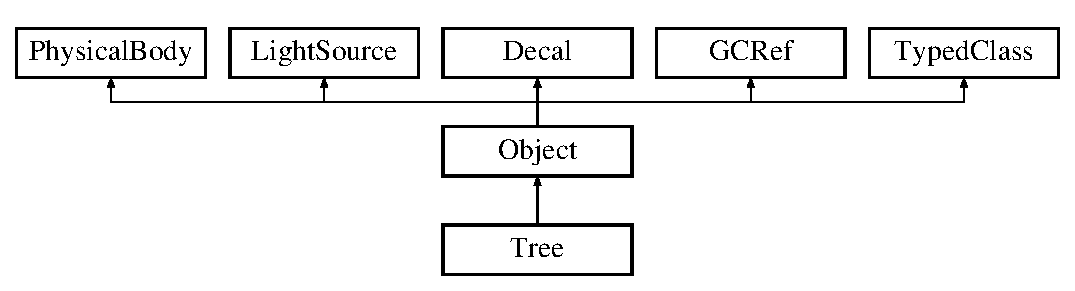
\includegraphics[height=3.000000cm]{classTree}
\end{center}
\end{figure}
\subsection*{Public Member Functions}
\begin{DoxyCompactItemize}
\item 
\hypertarget{classTree_ae87378915fea4c31cca95e768b62f2c1}{}{\bfseries Tree} (std\+::string n=\char`\"{}Tree\char`\"{})\label{classTree_ae87378915fea4c31cca95e768b62f2c1}

\end{DoxyCompactItemize}
\subsection*{Static Public Attributes}
\begin{DoxyCompactItemize}
\item 
\hypertarget{classTree_aaa9a72f41d4a4dbb7c86ddc8b1711473}{}static constexpr char $\ast$ {\bfseries type\+Name} =(char$\ast$)\char`\"{}Tree\char`\"{}\label{classTree_aaa9a72f41d4a4dbb7c86ddc8b1711473}

\end{DoxyCompactItemize}
\subsection*{Additional Inherited Members}


The documentation for this class was generated from the following files\+:\begin{DoxyCompactItemize}
\item 
drivers/include/Static.\+h\item 
drivers/src/Static.\+cpp\end{DoxyCompactItemize}

\hypertarget{classTypedClass}{}\section{Typed\+Class Class Reference}
\label{classTypedClass}\index{Typed\+Class@{Typed\+Class}}


The \hyperlink{classTypedClass}{Typed\+Class} class class meant to be inherited by classes meant to be downcasted, providing basic \char`\"{}instanceof\char`\"{} functionality.  




{\ttfamily \#include $<$utils.\+h$>$}

Inheritance diagram for Typed\+Class\+:\begin{figure}[H]
\begin{center}
\leavevmode
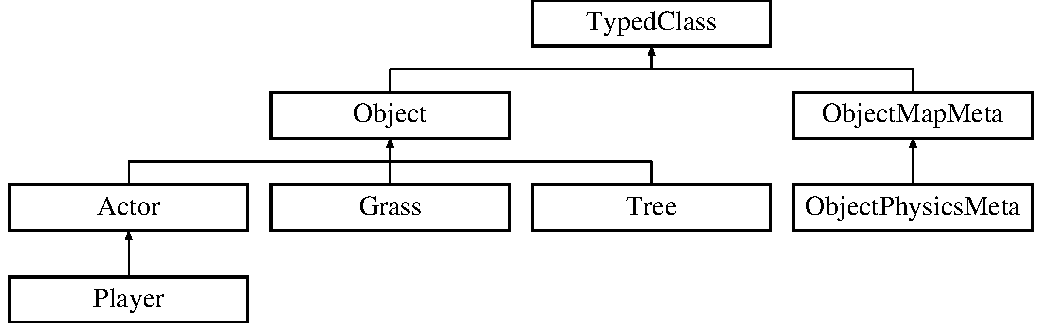
\includegraphics[height=3.472868cm]{classTypedClass}
\end{center}
\end{figure}
\subsection*{Public Member Functions}
\begin{DoxyCompactItemize}
\item 
const char $\ast$ \hyperlink{classTypedClass_ad12ee69d293a535940caea9cceea2659}{type\+Of} () const 
\begin{DoxyCompactList}\small\item\em type\+Of returns highest level type name \end{DoxyCompactList}\item 
bool \hyperlink{classTypedClass_a4af819bf3ec6b84e65c97fff993a1392}{match\+Type} (\hyperlink{classTypedClass}{Typed\+Class} \&t) const 
\begin{DoxyCompactList}\small\item\em match\+Type tells whether class is type as provided reference class \end{DoxyCompactList}\item 
bool \hyperlink{classTypedClass_ad31239a6b7d8eab7a63a8c28767e99e9}{match\+Type} (const char $\ast$type) const 
\begin{DoxyCompactList}\small\item\em match\+Type tells whether class is type as provided type descriptor \end{DoxyCompactList}\item 
bool \hyperlink{classTypedClass_a3b2358800578595aa3d490917431e19a}{is\+Type\+Of} (\hyperlink{classTypedClass}{Typed\+Class} \&t) const 
\begin{DoxyCompactList}\small\item\em is\+Type\+Of tells whether current class inherits from specified class \end{DoxyCompactList}\item 
bool \hyperlink{classTypedClass_ab4fc19854ea57d5055cd0d0e1baeec11}{is\+Type\+Of} (const char $\ast$type) const 
\begin{DoxyCompactList}\small\item\em is\+Type\+Of tells whether current class inherits from specified class descriptor \end{DoxyCompactList}\end{DoxyCompactItemize}
\subsection*{Static Public Attributes}
\begin{DoxyCompactItemize}
\item 
\hypertarget{classTypedClass_a14ef8946c4d5af21949bde220d686617}{}static constexpr char $\ast$ \hyperlink{classTypedClass_a14ef8946c4d5af21949bde220d686617}{type\+Name} =(char$\ast$)\char`\"{}Generic\char`\"{}\label{classTypedClass_a14ef8946c4d5af21949bde220d686617}

\begin{DoxyCompactList}\small\item\em type descriptor \end{DoxyCompactList}\end{DoxyCompactItemize}
\subsection*{Protected Member Functions}
\begin{DoxyCompactItemize}
\item 
void \hyperlink{classTypedClass_a39c4e5de4ad1bf09e24a5c4b6e56e506}{push\+Type} (const char $\ast$type)
\begin{DoxyCompactList}\small\item\em push\+Type Adds new type descriptor to registered inheritance tree \end{DoxyCompactList}\end{DoxyCompactItemize}


\subsection{Detailed Description}
The \hyperlink{classTypedClass}{Typed\+Class} class class meant to be inherited by classes meant to be downcasted, providing basic \char`\"{}instanceof\char`\"{} functionality. 

\subsection{Member Function Documentation}
\hypertarget{classTypedClass_a3b2358800578595aa3d490917431e19a}{}\index{Typed\+Class@{Typed\+Class}!is\+Type\+Of@{is\+Type\+Of}}
\index{is\+Type\+Of@{is\+Type\+Of}!Typed\+Class@{Typed\+Class}}
\subsubsection[{is\+Type\+Of}]{\setlength{\rightskip}{0pt plus 5cm}bool Typed\+Class\+::is\+Type\+Of (
\begin{DoxyParamCaption}
\item[{{\bf Typed\+Class} \&}]{t}
\end{DoxyParamCaption}
) const\hspace{0.3cm}{\ttfamily [inline]}}\label{classTypedClass_a3b2358800578595aa3d490917431e19a}


is\+Type\+Of tells whether current class inherits from specified class 


\begin{DoxyParams}{Parameters}
{\em t} & reference class \\
\hline
\end{DoxyParams}
\begin{DoxyReturn}{Returns}
yup or nope 
\end{DoxyReturn}
\hypertarget{classTypedClass_ab4fc19854ea57d5055cd0d0e1baeec11}{}\index{Typed\+Class@{Typed\+Class}!is\+Type\+Of@{is\+Type\+Of}}
\index{is\+Type\+Of@{is\+Type\+Of}!Typed\+Class@{Typed\+Class}}
\subsubsection[{is\+Type\+Of}]{\setlength{\rightskip}{0pt plus 5cm}bool Typed\+Class\+::is\+Type\+Of (
\begin{DoxyParamCaption}
\item[{const char $\ast$}]{type}
\end{DoxyParamCaption}
) const\hspace{0.3cm}{\ttfamily [inline]}}\label{classTypedClass_ab4fc19854ea57d5055cd0d0e1baeec11}


is\+Type\+Of tells whether current class inherits from specified class descriptor 


\begin{DoxyParams}{Parameters}
{\em type} & class descriptor \\
\hline
\end{DoxyParams}
\begin{DoxyReturn}{Returns}
yup or nope 
\end{DoxyReturn}
\hypertarget{classTypedClass_a4af819bf3ec6b84e65c97fff993a1392}{}\index{Typed\+Class@{Typed\+Class}!match\+Type@{match\+Type}}
\index{match\+Type@{match\+Type}!Typed\+Class@{Typed\+Class}}
\subsubsection[{match\+Type}]{\setlength{\rightskip}{0pt plus 5cm}bool Typed\+Class\+::match\+Type (
\begin{DoxyParamCaption}
\item[{{\bf Typed\+Class} \&}]{t}
\end{DoxyParamCaption}
) const\hspace{0.3cm}{\ttfamily [inline]}}\label{classTypedClass_a4af819bf3ec6b84e65c97fff993a1392}


match\+Type tells whether class is type as provided reference class 


\begin{DoxyParams}{Parameters}
{\em t} & class to be compared with \\
\hline
\end{DoxyParams}
\begin{DoxyReturn}{Returns}
yup or nope 
\end{DoxyReturn}
\hypertarget{classTypedClass_ad31239a6b7d8eab7a63a8c28767e99e9}{}\index{Typed\+Class@{Typed\+Class}!match\+Type@{match\+Type}}
\index{match\+Type@{match\+Type}!Typed\+Class@{Typed\+Class}}
\subsubsection[{match\+Type}]{\setlength{\rightskip}{0pt plus 5cm}bool Typed\+Class\+::match\+Type (
\begin{DoxyParamCaption}
\item[{const char $\ast$}]{type}
\end{DoxyParamCaption}
) const\hspace{0.3cm}{\ttfamily [inline]}}\label{classTypedClass_ad31239a6b7d8eab7a63a8c28767e99e9}


match\+Type tells whether class is type as provided type descriptor 


\begin{DoxyParams}{Parameters}
{\em type} & descriptor to be compared with \\
\hline
\end{DoxyParams}
\begin{DoxyReturn}{Returns}
yup or nope 
\end{DoxyReturn}
\hypertarget{classTypedClass_a39c4e5de4ad1bf09e24a5c4b6e56e506}{}\index{Typed\+Class@{Typed\+Class}!push\+Type@{push\+Type}}
\index{push\+Type@{push\+Type}!Typed\+Class@{Typed\+Class}}
\subsubsection[{push\+Type}]{\setlength{\rightskip}{0pt plus 5cm}void Typed\+Class\+::push\+Type (
\begin{DoxyParamCaption}
\item[{const char $\ast$}]{type}
\end{DoxyParamCaption}
)\hspace{0.3cm}{\ttfamily [inline]}, {\ttfamily [protected]}}\label{classTypedClass_a39c4e5de4ad1bf09e24a5c4b6e56e506}


push\+Type Adds new type descriptor to registered inheritance tree 


\begin{DoxyParams}{Parameters}
{\em type} & new class type descriptor \\
\hline
\end{DoxyParams}
\hypertarget{classTypedClass_ad12ee69d293a535940caea9cceea2659}{}\index{Typed\+Class@{Typed\+Class}!type\+Of@{type\+Of}}
\index{type\+Of@{type\+Of}!Typed\+Class@{Typed\+Class}}
\subsubsection[{type\+Of}]{\setlength{\rightskip}{0pt plus 5cm}const char$\ast$ Typed\+Class\+::type\+Of (
\begin{DoxyParamCaption}
{}
\end{DoxyParamCaption}
) const\hspace{0.3cm}{\ttfamily [inline]}}\label{classTypedClass_ad12ee69d293a535940caea9cceea2659}


type\+Of returns highest level type name 

\begin{DoxyReturn}{Returns}
type name 
\end{DoxyReturn}


The documentation for this class was generated from the following files\+:\begin{DoxyCompactItemize}
\item 
include/utils.\+h\item 
src/utils.\+cpp\end{DoxyCompactItemize}

\hypertarget{classVectorXY}{}\section{Vector\+X\+Y Class Reference}
\label{classVectorXY}\index{Vector\+X\+Y@{Vector\+X\+Y}}


The \hyperlink{classVectorXY}{Vector\+X\+Y} class Class providing basic vector functionality.  




{\ttfamily \#include $<$Vector\+X\+Y.\+h$>$}

\subsection*{Public Member Functions}
\begin{DoxyCompactItemize}
\item 
\hyperlink{classVectorXY_a8cf9a7bae3f5c6c120f305268076a2af}{Vector\+X\+Y} (long double x\+Beg=0, long double y\+Beg=0, long double x\+End=1, long double y\+End=1)
\begin{DoxyCompactList}\small\item\em $<$ vector end \end{DoxyCompactList}\item 
\hyperlink{classVectorXY_a1d6f51eec2d1eb3d4f70d3c6d9c6bed1}{Vector\+X\+Y} (const \hyperlink{classPointXY}{Point\+X\+Y} \&first, const \hyperlink{classPointXY}{Point\+X\+Y} \&last)
\begin{DoxyCompactList}\small\item\em \hyperlink{classVectorXY}{Vector\+X\+Y} constructor from points. \end{DoxyCompactList}\item 
\hyperlink{classVectorXY_afa7511b9ada046d507e11acbdca41a0b}{Vector\+X\+Y} (const \hyperlink{classVectorXY}{Vector\+X\+Y} \&tmp)
\begin{DoxyCompactList}\small\item\em \hyperlink{classVectorXY}{Vector\+X\+Y} copy constructor. \end{DoxyCompactList}\item 
const \hyperlink{classPointXY}{Point\+X\+Y} \& \hyperlink{classVectorXY_a756a3c349a46361ce94af16a358d0699}{get\+Begin} () const 
\begin{DoxyCompactList}\small\item\em get\+Begin \end{DoxyCompactList}\item 
const \hyperlink{classPointXY}{Point\+X\+Y} \& \hyperlink{classVectorXY_a59ba6208946c4860c43f84a11f2d4ca4}{get\+End} () const 
\begin{DoxyCompactList}\small\item\em get\+End \end{DoxyCompactList}\item 
void \hyperlink{classVectorXY_a54d01726e2920265ddc17152d292ad3e}{set\+Begin} (const \hyperlink{classPointXY}{Point\+X\+Y} \&A)
\begin{DoxyCompactList}\small\item\em set\+Begin set beginning point of vector to specified value \end{DoxyCompactList}\item 
\hypertarget{classVectorXY_ab72566580ee7cfbd9dae6c9b89ba1245}{}void {\bfseries set\+Begin} (long double a, long double b)\label{classVectorXY_ab72566580ee7cfbd9dae6c9b89ba1245}

\item 
void \hyperlink{classVectorXY_a4aa9560ca31838238992c604f23c1910}{set\+End} (const \hyperlink{classPointXY}{Point\+X\+Y} \&A)
\begin{DoxyCompactList}\small\item\em set\+End set endinf point of vector to specified value \end{DoxyCompactList}\item 
\hypertarget{classVectorXY_a808bcf64655761e98f92e915ba6bd634}{}void {\bfseries set\+End} (long double a, long double b)\label{classVectorXY_a808bcf64655761e98f92e915ba6bd634}

\item 
void \hyperlink{classVectorXY_a8ba83cb02ebe32672926abac17ab174e}{set\+Vector} (const \hyperlink{classPointXY}{Point\+X\+Y} \&beg, const \hyperlink{classPointXY}{Point\+X\+Y} \&end)
\begin{DoxyCompactList}\small\item\em set\+Vector set vector to new one \end{DoxyCompactList}\item 
long double \hyperlink{classVectorXY_adb8b4da2bd2d7383af3973d6daa95b53}{height} () const 
\begin{DoxyCompactList}\small\item\em height returns height of vector (Y axis length) \end{DoxyCompactList}\item 
long double \hyperlink{classVectorXY_ada8c272d3a9f8aab0b6af4cd15763d23}{width} () const 
\begin{DoxyCompactList}\small\item\em width returns width of vector (X axis length) \end{DoxyCompactList}\item 
\hyperlink{classPointXY}{Point\+X\+Y} \hyperlink{classVectorXY_a0f1457e18bad227f3e06b5b3ca37f0b7}{size\+X\+Y} () const 
\begin{DoxyCompactList}\small\item\em size\+X\+Y returns pair of width\+:heigth as Point class \end{DoxyCompactList}\item 
long double \hyperlink{classVectorXY_aa7aa129411aaeb43a1b89084c2af5da8}{size} () const 
\begin{DoxyCompactList}\small\item\em size Euclidean length of vector \end{DoxyCompactList}\item 
void \hyperlink{classVectorXY_a85281070287140c27325ad11e7198840}{move\+To} (long double x, long double y, bool end=false)
\begin{DoxyCompactList}\small\item\em move\+To move vector to specified position \end{DoxyCompactList}\item 
void \hyperlink{classVectorXY_a27649ddf218ed91b6c38e9ccee45a637}{move\+By} (long double x, long double y)
\begin{DoxyCompactList}\small\item\em move\+By move vector by specified offset \end{DoxyCompactList}\item 
\hypertarget{classVectorXY_a10fb6ca1d0a636852eff2f753b619ac8}{}void {\bfseries move\+By} (\hyperlink{classPointXY}{Point\+X\+Y} \&point)\label{classVectorXY_a10fb6ca1d0a636852eff2f753b619ac8}

\item 
void \hyperlink{classVectorXY_a55713178bb2845a83b858c5776194b6d}{center\+On} (long double x, long double y)
\begin{DoxyCompactList}\small\item\em center\+On center vector on specified point \end{DoxyCompactList}\item 
\hypertarget{classVectorXY_a2ff78c91d0896f2d32aba1d612b4e7e0}{}void {\bfseries center\+On} (\hyperlink{classPointXY}{Point\+X\+Y} \&point)\label{classVectorXY_a2ff78c91d0896f2d32aba1d612b4e7e0}

\item 
void \hyperlink{classVectorXY_a92c5fd3e5018183f59e409abd523b23b}{scale\+By} (long double k)
\begin{DoxyCompactList}\small\item\em scale\+By scale vector by specified fraction (from point 0,0) \end{DoxyCompactList}\item 
void \hyperlink{classVectorXY_a08ef32c78e917db26296e27a924504bf}{scale\+To} (long double siz)
\begin{DoxyCompactList}\small\item\em scale\+To scale vector to specified Euclidean length (from point 0,0) \end{DoxyCompactList}\item 
void \hyperlink{classVectorXY_a6cc6d38fbe0d949a6758d6b04ff61818}{scale\+Length\+To} (long double k, bool end=false)
\begin{DoxyCompactList}\small\item\em scale\+Length\+To scale vector by specified fraction (from beginning point) \end{DoxyCompactList}\item 
void \hyperlink{classVectorXY_aa4dfb1630e9d1b440a7f383a8f7f5bd8}{scale\+Length\+By} (long double k, bool end=false)
\begin{DoxyCompactList}\small\item\em scale\+Length\+By scale vector to specified Euclidean length (from point 0,0) \end{DoxyCompactList}\item 
\hypertarget{classVectorXY_a6d9d6f426a7dd4135a088da08823f371}{}void \hyperlink{classVectorXY_a6d9d6f426a7dd4135a088da08823f371}{flip} ()\label{classVectorXY_a6d9d6f426a7dd4135a088da08823f371}

\begin{DoxyCompactList}\small\item\em flip swap beginning point with ending one \end{DoxyCompactList}\item 
\hypertarget{classVectorXY_a5a65769eeb23d8c5d2deb0ef821777d9}{}\hyperlink{classVectorXY}{Vector\+X\+Y} {\bfseries operator+} (\hyperlink{classVectorXY}{Vector\+X\+Y} vect) const \label{classVectorXY_a5a65769eeb23d8c5d2deb0ef821777d9}

\item 
\hypertarget{classVectorXY_a3e9b238c7a3a7c1dbffd02b841d32926}{}\hyperlink{classVectorXY}{Vector\+X\+Y} {\bfseries operator-\/} (\hyperlink{classVectorXY}{Vector\+X\+Y} vect) const \label{classVectorXY_a3e9b238c7a3a7c1dbffd02b841d32926}

\item 
\hypertarget{classVectorXY_a7206b9e67b835aa3d1bc02d58593e89d}{}void {\bfseries operator+=} (\hyperlink{classVectorXY}{Vector\+X\+Y} vect)\label{classVectorXY_a7206b9e67b835aa3d1bc02d58593e89d}

\item 
\hypertarget{classVectorXY_a4849b9c7d700cb33819fd9a67a7bdb65}{}void {\bfseries operator-\/=} (\hyperlink{classVectorXY}{Vector\+X\+Y} vect)\label{classVectorXY_a4849b9c7d700cb33819fd9a67a7bdb65}

\item 
\hypertarget{classVectorXY_aa54d52ee35bd9f23aacf9e40db864afe}{}\hyperlink{classVectorXY}{Vector\+X\+Y} {\bfseries operator$\ast$} (double k) const \label{classVectorXY_aa54d52ee35bd9f23aacf9e40db864afe}

\item 
\hypertarget{classVectorXY_aca23f07f70da97399ad83d6c1d025420}{}void {\bfseries operator$\ast$=} (double k)\label{classVectorXY_aca23f07f70da97399ad83d6c1d025420}

\item 
\hypertarget{classVectorXY_af815be1ddb6c8d4e9222791240549fbf}{}bool {\bfseries operator==} (const \hyperlink{classVectorXY}{Vector\+X\+Y} \&vect) const \label{classVectorXY_af815be1ddb6c8d4e9222791240549fbf}

\item 
\hypertarget{classVectorXY_ad288ee31a7ef0437962779fd631acd23}{}bool {\bfseries operator!=} (const \hyperlink{classVectorXY}{Vector\+X\+Y} \&vect) const \label{classVectorXY_ad288ee31a7ef0437962779fd631acd23}

\end{DoxyCompactItemize}
\subsection*{Static Public Member Functions}
\begin{DoxyCompactItemize}
\item 
static bool \hyperlink{classVectorXY_a585c00eaedb3c0af026cca3d155df34d}{intersects} (const \hyperlink{classVectorXY}{Vector\+X\+Y} \&A, const \hyperlink{classVectorXY}{Vector\+X\+Y} \&B)
\begin{DoxyCompactList}\small\item\em intersects indicates whether 2 vectors intersect or not \end{DoxyCompactList}\item 
static long double \hyperlink{classVectorXY_afd36ee1e0721ed9aea5cf47dbbca6f66}{scalar\+Product} (\hyperlink{classPointXY}{Point\+X\+Y} $\ast$a, \hyperlink{classPointXY}{Point\+X\+Y} $\ast$b, \hyperlink{classPointXY}{Point\+X\+Y} $\ast$c)
\begin{DoxyCompactList}\small\item\em scalar\+Product scalar product of 2 detached vector \end{DoxyCompactList}\item 
static void \hyperlink{classVectorXY_a61f4148fb8478296adb53e3f11e35bce}{flip\+Across\+Vector} (\hyperlink{classVectorXY}{Vector\+X\+Y} \&A, \hyperlink{classVectorXY}{Vector\+X\+Y} \&B)
\begin{DoxyCompactList}\small\item\em flip\+Across\+Vector flip one vector across another \end{DoxyCompactList}\item 
static void \hyperlink{classVectorXY_a07353914e6a38ea4426314d3997234e6}{flip\+Across\+Vector} (\hyperlink{classPointXY}{Point\+X\+Y} \&pt, \hyperlink{classVectorXY}{Vector\+X\+Y} \&vec)
\begin{DoxyCompactList}\small\item\em flip\+Across\+Vector flip point actoss vector \end{DoxyCompactList}\item 
static void \hyperlink{classVectorXY_a62651da7f0e1ef8cad09fb48e05488c4}{project\+Onto\+Vector} (\hyperlink{classPointXY}{Point\+X\+Y} \&pt, \hyperlink{classVectorXY}{Vector\+X\+Y} \&vec)
\begin{DoxyCompactList}\small\item\em project\+Onto\+Vector projectile point onto vector \end{DoxyCompactList}\item 
static void \hyperlink{classVectorXY_a79bb35dc0ea4090c75ed95123cb2c7f9}{project\+Onto\+Vector} (\hyperlink{classVectorXY}{Vector\+X\+Y} \&A, \hyperlink{classVectorXY}{Vector\+X\+Y} \&B)
\begin{DoxyCompactList}\small\item\em project\+Onto\+Vector projectile vector onto another vector \end{DoxyCompactList}\end{DoxyCompactItemize}
\subsection*{Friends}
\begin{DoxyCompactItemize}
\item 
\hypertarget{classVectorXY_acaa3c11c02bd1fe1fb410ee45b028c87}{}\hyperlink{classVectorXY}{Vector\+X\+Y} {\bfseries operator$\ast$} (const double \&k, const \hyperlink{classVectorXY}{Vector\+X\+Y} \&vect)\label{classVectorXY_acaa3c11c02bd1fe1fb410ee45b028c87}

\end{DoxyCompactItemize}


\subsection{Detailed Description}
The \hyperlink{classVectorXY}{Vector\+X\+Y} class Class providing basic vector functionality. 

\subsection{Constructor \& Destructor Documentation}
\hypertarget{classVectorXY_a8cf9a7bae3f5c6c120f305268076a2af}{}\index{Vector\+X\+Y@{Vector\+X\+Y}!Vector\+X\+Y@{Vector\+X\+Y}}
\index{Vector\+X\+Y@{Vector\+X\+Y}!Vector\+X\+Y@{Vector\+X\+Y}}
\subsubsection[{Vector\+X\+Y}]{\setlength{\rightskip}{0pt plus 5cm}Vector\+X\+Y\+::\+Vector\+X\+Y (
\begin{DoxyParamCaption}
\item[{long double}]{x\+Beg = {\ttfamily 0}, }
\item[{long double}]{y\+Beg = {\ttfamily 0}, }
\item[{long double}]{x\+End = {\ttfamily 1}, }
\item[{long double}]{y\+End = {\ttfamily 1}}
\end{DoxyParamCaption}
)}\label{classVectorXY_a8cf9a7bae3f5c6c120f305268076a2af}


$<$ vector end 

\hyperlink{classVectorXY}{Vector\+X\+Y} basic constructor 
\begin{DoxyParams}{Parameters}
{\em x\+Beg} & x begin \\
\hline
{\em y\+Beg} & y begin \\
\hline
{\em x\+End} & x end \\
\hline
{\em y\+End} & y end \\
\hline
\end{DoxyParams}
\hypertarget{classVectorXY_a1d6f51eec2d1eb3d4f70d3c6d9c6bed1}{}\index{Vector\+X\+Y@{Vector\+X\+Y}!Vector\+X\+Y@{Vector\+X\+Y}}
\index{Vector\+X\+Y@{Vector\+X\+Y}!Vector\+X\+Y@{Vector\+X\+Y}}
\subsubsection[{Vector\+X\+Y}]{\setlength{\rightskip}{0pt plus 5cm}Vector\+X\+Y\+::\+Vector\+X\+Y (
\begin{DoxyParamCaption}
\item[{const {\bf Point\+X\+Y} \&}]{first, }
\item[{const {\bf Point\+X\+Y} \&}]{last}
\end{DoxyParamCaption}
)}\label{classVectorXY_a1d6f51eec2d1eb3d4f70d3c6d9c6bed1}


\hyperlink{classVectorXY}{Vector\+X\+Y} constructor from points. 


\begin{DoxyParams}{Parameters}
{\em first} & begin \\
\hline
{\em last} & end \\
\hline
\end{DoxyParams}
\hypertarget{classVectorXY_afa7511b9ada046d507e11acbdca41a0b}{}\index{Vector\+X\+Y@{Vector\+X\+Y}!Vector\+X\+Y@{Vector\+X\+Y}}
\index{Vector\+X\+Y@{Vector\+X\+Y}!Vector\+X\+Y@{Vector\+X\+Y}}
\subsubsection[{Vector\+X\+Y}]{\setlength{\rightskip}{0pt plus 5cm}Vector\+X\+Y\+::\+Vector\+X\+Y (
\begin{DoxyParamCaption}
\item[{const {\bf Vector\+X\+Y} \&}]{tmp}
\end{DoxyParamCaption}
)}\label{classVectorXY_afa7511b9ada046d507e11acbdca41a0b}


\hyperlink{classVectorXY}{Vector\+X\+Y} copy constructor. 


\begin{DoxyParams}{Parameters}
{\em tmp} & reference \\
\hline
\end{DoxyParams}


\subsection{Member Function Documentation}
\hypertarget{classVectorXY_a55713178bb2845a83b858c5776194b6d}{}\index{Vector\+X\+Y@{Vector\+X\+Y}!center\+On@{center\+On}}
\index{center\+On@{center\+On}!Vector\+X\+Y@{Vector\+X\+Y}}
\subsubsection[{center\+On}]{\setlength{\rightskip}{0pt plus 5cm}void Vector\+X\+Y\+::center\+On (
\begin{DoxyParamCaption}
\item[{long double}]{x, }
\item[{long double}]{y}
\end{DoxyParamCaption}
)}\label{classVectorXY_a55713178bb2845a83b858c5776194b6d}


center\+On center vector on specified point 


\begin{DoxyParams}{Parameters}
{\em x} & desired x \\
\hline
{\em y} & desired y \\
\hline
\end{DoxyParams}
\hypertarget{classVectorXY_a61f4148fb8478296adb53e3f11e35bce}{}\index{Vector\+X\+Y@{Vector\+X\+Y}!flip\+Across\+Vector@{flip\+Across\+Vector}}
\index{flip\+Across\+Vector@{flip\+Across\+Vector}!Vector\+X\+Y@{Vector\+X\+Y}}
\subsubsection[{flip\+Across\+Vector}]{\setlength{\rightskip}{0pt plus 5cm}void Vector\+X\+Y\+::flip\+Across\+Vector (
\begin{DoxyParamCaption}
\item[{{\bf Vector\+X\+Y} \&}]{A, }
\item[{{\bf Vector\+X\+Y} \&}]{B}
\end{DoxyParamCaption}
)\hspace{0.3cm}{\ttfamily [static]}}\label{classVectorXY_a61f4148fb8478296adb53e3f11e35bce}


flip\+Across\+Vector flip one vector across another 


\begin{DoxyParams}{Parameters}
{\em A} & vector to be flipped \\
\hline
{\em B} & vector to flip against \\
\hline
\end{DoxyParams}
\hypertarget{classVectorXY_a07353914e6a38ea4426314d3997234e6}{}\index{Vector\+X\+Y@{Vector\+X\+Y}!flip\+Across\+Vector@{flip\+Across\+Vector}}
\index{flip\+Across\+Vector@{flip\+Across\+Vector}!Vector\+X\+Y@{Vector\+X\+Y}}
\subsubsection[{flip\+Across\+Vector}]{\setlength{\rightskip}{0pt plus 5cm}void Vector\+X\+Y\+::flip\+Across\+Vector (
\begin{DoxyParamCaption}
\item[{{\bf Point\+X\+Y} \&}]{pt, }
\item[{{\bf Vector\+X\+Y} \&}]{vec}
\end{DoxyParamCaption}
)\hspace{0.3cm}{\ttfamily [static]}}\label{classVectorXY_a07353914e6a38ea4426314d3997234e6}


flip\+Across\+Vector flip point actoss vector 


\begin{DoxyParams}{Parameters}
{\em pt} & point \\
\hline
{\em vec} & vector \\
\hline
\end{DoxyParams}
\hypertarget{classVectorXY_a756a3c349a46361ce94af16a358d0699}{}\index{Vector\+X\+Y@{Vector\+X\+Y}!get\+Begin@{get\+Begin}}
\index{get\+Begin@{get\+Begin}!Vector\+X\+Y@{Vector\+X\+Y}}
\subsubsection[{get\+Begin}]{\setlength{\rightskip}{0pt plus 5cm}const {\bf Point\+X\+Y}\& Vector\+X\+Y\+::get\+Begin (
\begin{DoxyParamCaption}
{}
\end{DoxyParamCaption}
) const\hspace{0.3cm}{\ttfamily [inline]}}\label{classVectorXY_a756a3c349a46361ce94af16a358d0699}


get\+Begin 

\begin{DoxyReturn}{Returns}
begin of vector 
\end{DoxyReturn}
\hypertarget{classVectorXY_a59ba6208946c4860c43f84a11f2d4ca4}{}\index{Vector\+X\+Y@{Vector\+X\+Y}!get\+End@{get\+End}}
\index{get\+End@{get\+End}!Vector\+X\+Y@{Vector\+X\+Y}}
\subsubsection[{get\+End}]{\setlength{\rightskip}{0pt plus 5cm}const {\bf Point\+X\+Y}\& Vector\+X\+Y\+::get\+End (
\begin{DoxyParamCaption}
{}
\end{DoxyParamCaption}
) const\hspace{0.3cm}{\ttfamily [inline]}}\label{classVectorXY_a59ba6208946c4860c43f84a11f2d4ca4}


get\+End 

\begin{DoxyReturn}{Returns}
end of vector 
\end{DoxyReturn}
\hypertarget{classVectorXY_adb8b4da2bd2d7383af3973d6daa95b53}{}\index{Vector\+X\+Y@{Vector\+X\+Y}!height@{height}}
\index{height@{height}!Vector\+X\+Y@{Vector\+X\+Y}}
\subsubsection[{height}]{\setlength{\rightskip}{0pt plus 5cm}long double Vector\+X\+Y\+::height (
\begin{DoxyParamCaption}
{}
\end{DoxyParamCaption}
) const}\label{classVectorXY_adb8b4da2bd2d7383af3973d6daa95b53}


height returns height of vector (Y axis length) 

\begin{DoxyReturn}{Returns}
height of vector 
\end{DoxyReturn}
\hypertarget{classVectorXY_a585c00eaedb3c0af026cca3d155df34d}{}\index{Vector\+X\+Y@{Vector\+X\+Y}!intersects@{intersects}}
\index{intersects@{intersects}!Vector\+X\+Y@{Vector\+X\+Y}}
\subsubsection[{intersects}]{\setlength{\rightskip}{0pt plus 5cm}bool Vector\+X\+Y\+::intersects (
\begin{DoxyParamCaption}
\item[{const {\bf Vector\+X\+Y} \&}]{A, }
\item[{const {\bf Vector\+X\+Y} \&}]{B}
\end{DoxyParamCaption}
)\hspace{0.3cm}{\ttfamily [static]}}\label{classVectorXY_a585c00eaedb3c0af026cca3d155df34d}


intersects indicates whether 2 vectors intersect or not 


\begin{DoxyParams}{Parameters}
{\em A} & vector A \\
\hline
{\em B} & vector B \\
\hline
\end{DoxyParams}
\begin{DoxyReturn}{Returns}
whether A intersects with B 
\end{DoxyReturn}
\hypertarget{classVectorXY_a27649ddf218ed91b6c38e9ccee45a637}{}\index{Vector\+X\+Y@{Vector\+X\+Y}!move\+By@{move\+By}}
\index{move\+By@{move\+By}!Vector\+X\+Y@{Vector\+X\+Y}}
\subsubsection[{move\+By}]{\setlength{\rightskip}{0pt plus 5cm}void Vector\+X\+Y\+::move\+By (
\begin{DoxyParamCaption}
\item[{long double}]{x, }
\item[{long double}]{y}
\end{DoxyParamCaption}
)}\label{classVectorXY_a27649ddf218ed91b6c38e9ccee45a637}


move\+By move vector by specified offset 


\begin{DoxyParams}{Parameters}
{\em x} & x offset \\
\hline
{\em y} & y offset \\
\hline
\end{DoxyParams}
\hypertarget{classVectorXY_a85281070287140c27325ad11e7198840}{}\index{Vector\+X\+Y@{Vector\+X\+Y}!move\+To@{move\+To}}
\index{move\+To@{move\+To}!Vector\+X\+Y@{Vector\+X\+Y}}
\subsubsection[{move\+To}]{\setlength{\rightskip}{0pt plus 5cm}void Vector\+X\+Y\+::move\+To (
\begin{DoxyParamCaption}
\item[{long double}]{x, }
\item[{long double}]{y, }
\item[{bool}]{end = {\ttfamily false}}
\end{DoxyParamCaption}
)}\label{classVectorXY_a85281070287140c27325ad11e7198840}


move\+To move vector to specified position 


\begin{DoxyParams}{Parameters}
{\em x} & desired x pos \\
\hline
{\em y} & desired y pos \\
\hline
{\em end} & flag indicating which point of vector should be aligned \\
\hline
\end{DoxyParams}
\hypertarget{classVectorXY_a62651da7f0e1ef8cad09fb48e05488c4}{}\index{Vector\+X\+Y@{Vector\+X\+Y}!project\+Onto\+Vector@{project\+Onto\+Vector}}
\index{project\+Onto\+Vector@{project\+Onto\+Vector}!Vector\+X\+Y@{Vector\+X\+Y}}
\subsubsection[{project\+Onto\+Vector}]{\setlength{\rightskip}{0pt plus 5cm}void Vector\+X\+Y\+::project\+Onto\+Vector (
\begin{DoxyParamCaption}
\item[{{\bf Point\+X\+Y} \&}]{pt, }
\item[{{\bf Vector\+X\+Y} \&}]{vec}
\end{DoxyParamCaption}
)\hspace{0.3cm}{\ttfamily [static]}}\label{classVectorXY_a62651da7f0e1ef8cad09fb48e05488c4}


project\+Onto\+Vector projectile point onto vector 


\begin{DoxyParams}{Parameters}
{\em pt} & point \\
\hline
{\em vec} & vector \\
\hline
\end{DoxyParams}
\hypertarget{classVectorXY_a79bb35dc0ea4090c75ed95123cb2c7f9}{}\index{Vector\+X\+Y@{Vector\+X\+Y}!project\+Onto\+Vector@{project\+Onto\+Vector}}
\index{project\+Onto\+Vector@{project\+Onto\+Vector}!Vector\+X\+Y@{Vector\+X\+Y}}
\subsubsection[{project\+Onto\+Vector}]{\setlength{\rightskip}{0pt plus 5cm}void Vector\+X\+Y\+::project\+Onto\+Vector (
\begin{DoxyParamCaption}
\item[{{\bf Vector\+X\+Y} \&}]{A, }
\item[{{\bf Vector\+X\+Y} \&}]{B}
\end{DoxyParamCaption}
)\hspace{0.3cm}{\ttfamily [static]}}\label{classVectorXY_a79bb35dc0ea4090c75ed95123cb2c7f9}


project\+Onto\+Vector projectile vector onto another vector 


\begin{DoxyParams}{Parameters}
{\em A} & vector to be projected \\
\hline
{\em B} & vector to be projected on \\
\hline
\end{DoxyParams}
\hypertarget{classVectorXY_afd36ee1e0721ed9aea5cf47dbbca6f66}{}\index{Vector\+X\+Y@{Vector\+X\+Y}!scalar\+Product@{scalar\+Product}}
\index{scalar\+Product@{scalar\+Product}!Vector\+X\+Y@{Vector\+X\+Y}}
\subsubsection[{scalar\+Product}]{\setlength{\rightskip}{0pt plus 5cm}long double Vector\+X\+Y\+::scalar\+Product (
\begin{DoxyParamCaption}
\item[{{\bf Point\+X\+Y} $\ast$}]{a, }
\item[{{\bf Point\+X\+Y} $\ast$}]{b, }
\item[{{\bf Point\+X\+Y} $\ast$}]{c}
\end{DoxyParamCaption}
)\hspace{0.3cm}{\ttfamily [static]}}\label{classVectorXY_afd36ee1e0721ed9aea5cf47dbbca6f66}


scalar\+Product scalar product of 2 detached vector 


\begin{DoxyParams}{Parameters}
{\em a} & point A \\
\hline
{\em b} & commont point of 2 vectors \\
\hline
{\em c} & point B \\
\hline
\end{DoxyParams}
\begin{DoxyReturn}{Returns}

\end{DoxyReturn}
\hypertarget{classVectorXY_a92c5fd3e5018183f59e409abd523b23b}{}\index{Vector\+X\+Y@{Vector\+X\+Y}!scale\+By@{scale\+By}}
\index{scale\+By@{scale\+By}!Vector\+X\+Y@{Vector\+X\+Y}}
\subsubsection[{scale\+By}]{\setlength{\rightskip}{0pt plus 5cm}void Vector\+X\+Y\+::scale\+By (
\begin{DoxyParamCaption}
\item[{long double}]{k}
\end{DoxyParamCaption}
)}\label{classVectorXY_a92c5fd3e5018183f59e409abd523b23b}


scale\+By scale vector by specified fraction (from point 0,0) 


\begin{DoxyParams}{Parameters}
{\em k} & fraction \\
\hline
\end{DoxyParams}
\hypertarget{classVectorXY_aa4dfb1630e9d1b440a7f383a8f7f5bd8}{}\index{Vector\+X\+Y@{Vector\+X\+Y}!scale\+Length\+By@{scale\+Length\+By}}
\index{scale\+Length\+By@{scale\+Length\+By}!Vector\+X\+Y@{Vector\+X\+Y}}
\subsubsection[{scale\+Length\+By}]{\setlength{\rightskip}{0pt plus 5cm}void Vector\+X\+Y\+::scale\+Length\+By (
\begin{DoxyParamCaption}
\item[{long double}]{k, }
\item[{bool}]{end = {\ttfamily false}}
\end{DoxyParamCaption}
)}\label{classVectorXY_aa4dfb1630e9d1b440a7f383a8f7f5bd8}


scale\+Length\+By scale vector to specified Euclidean length (from point 0,0) 


\begin{DoxyParams}{Parameters}
{\em k} & \\
\hline
{\em end} & \\
\hline
\end{DoxyParams}
\hypertarget{classVectorXY_a6cc6d38fbe0d949a6758d6b04ff61818}{}\index{Vector\+X\+Y@{Vector\+X\+Y}!scale\+Length\+To@{scale\+Length\+To}}
\index{scale\+Length\+To@{scale\+Length\+To}!Vector\+X\+Y@{Vector\+X\+Y}}
\subsubsection[{scale\+Length\+To}]{\setlength{\rightskip}{0pt plus 5cm}void Vector\+X\+Y\+::scale\+Length\+To (
\begin{DoxyParamCaption}
\item[{long double}]{k, }
\item[{bool}]{end = {\ttfamily false}}
\end{DoxyParamCaption}
)}\label{classVectorXY_a6cc6d38fbe0d949a6758d6b04ff61818}


scale\+Length\+To scale vector by specified fraction (from beginning point) 


\begin{DoxyParams}{Parameters}
{\em k} & \\
\hline
{\em end} & \\
\hline
\end{DoxyParams}
\hypertarget{classVectorXY_a08ef32c78e917db26296e27a924504bf}{}\index{Vector\+X\+Y@{Vector\+X\+Y}!scale\+To@{scale\+To}}
\index{scale\+To@{scale\+To}!Vector\+X\+Y@{Vector\+X\+Y}}
\subsubsection[{scale\+To}]{\setlength{\rightskip}{0pt plus 5cm}void Vector\+X\+Y\+::scale\+To (
\begin{DoxyParamCaption}
\item[{long double}]{siz}
\end{DoxyParamCaption}
)}\label{classVectorXY_a08ef32c78e917db26296e27a924504bf}


scale\+To scale vector to specified Euclidean length (from point 0,0) 


\begin{DoxyParams}{Parameters}
{\em siz} & desired size \\
\hline
\end{DoxyParams}
\hypertarget{classVectorXY_a54d01726e2920265ddc17152d292ad3e}{}\index{Vector\+X\+Y@{Vector\+X\+Y}!set\+Begin@{set\+Begin}}
\index{set\+Begin@{set\+Begin}!Vector\+X\+Y@{Vector\+X\+Y}}
\subsubsection[{set\+Begin}]{\setlength{\rightskip}{0pt plus 5cm}void Vector\+X\+Y\+::set\+Begin (
\begin{DoxyParamCaption}
\item[{const {\bf Point\+X\+Y} \&}]{A}
\end{DoxyParamCaption}
)}\label{classVectorXY_a54d01726e2920265ddc17152d292ad3e}


set\+Begin set beginning point of vector to specified value 


\begin{DoxyParams}{Parameters}
{\em A} & new value \\
\hline
\end{DoxyParams}
\hypertarget{classVectorXY_a4aa9560ca31838238992c604f23c1910}{}\index{Vector\+X\+Y@{Vector\+X\+Y}!set\+End@{set\+End}}
\index{set\+End@{set\+End}!Vector\+X\+Y@{Vector\+X\+Y}}
\subsubsection[{set\+End}]{\setlength{\rightskip}{0pt plus 5cm}void Vector\+X\+Y\+::set\+End (
\begin{DoxyParamCaption}
\item[{const {\bf Point\+X\+Y} \&}]{A}
\end{DoxyParamCaption}
)}\label{classVectorXY_a4aa9560ca31838238992c604f23c1910}


set\+End set endinf point of vector to specified value 


\begin{DoxyParams}{Parameters}
{\em A} & new value \\
\hline
\end{DoxyParams}
\hypertarget{classVectorXY_a8ba83cb02ebe32672926abac17ab174e}{}\index{Vector\+X\+Y@{Vector\+X\+Y}!set\+Vector@{set\+Vector}}
\index{set\+Vector@{set\+Vector}!Vector\+X\+Y@{Vector\+X\+Y}}
\subsubsection[{set\+Vector}]{\setlength{\rightskip}{0pt plus 5cm}void Vector\+X\+Y\+::set\+Vector (
\begin{DoxyParamCaption}
\item[{const {\bf Point\+X\+Y} \&}]{beg, }
\item[{const {\bf Point\+X\+Y} \&}]{end}
\end{DoxyParamCaption}
)}\label{classVectorXY_a8ba83cb02ebe32672926abac17ab174e}


set\+Vector set vector to new one 


\begin{DoxyParams}{Parameters}
{\em beg} & new beginning \\
\hline
{\em end} & new ending \\
\hline
\end{DoxyParams}
\hypertarget{classVectorXY_aa7aa129411aaeb43a1b89084c2af5da8}{}\index{Vector\+X\+Y@{Vector\+X\+Y}!size@{size}}
\index{size@{size}!Vector\+X\+Y@{Vector\+X\+Y}}
\subsubsection[{size}]{\setlength{\rightskip}{0pt plus 5cm}long double Vector\+X\+Y\+::size (
\begin{DoxyParamCaption}
{}
\end{DoxyParamCaption}
) const}\label{classVectorXY_aa7aa129411aaeb43a1b89084c2af5da8}


size Euclidean length of vector 

\begin{DoxyReturn}{Returns}
length 
\end{DoxyReturn}
\hypertarget{classVectorXY_a0f1457e18bad227f3e06b5b3ca37f0b7}{}\index{Vector\+X\+Y@{Vector\+X\+Y}!size\+X\+Y@{size\+X\+Y}}
\index{size\+X\+Y@{size\+X\+Y}!Vector\+X\+Y@{Vector\+X\+Y}}
\subsubsection[{size\+X\+Y}]{\setlength{\rightskip}{0pt plus 5cm}{\bf Point\+X\+Y} Vector\+X\+Y\+::size\+X\+Y (
\begin{DoxyParamCaption}
{}
\end{DoxyParamCaption}
) const}\label{classVectorXY_a0f1457e18bad227f3e06b5b3ca37f0b7}


size\+X\+Y returns pair of width\+:heigth as Point class 

\begin{DoxyReturn}{Returns}
xy size 
\end{DoxyReturn}
\hypertarget{classVectorXY_ada8c272d3a9f8aab0b6af4cd15763d23}{}\index{Vector\+X\+Y@{Vector\+X\+Y}!width@{width}}
\index{width@{width}!Vector\+X\+Y@{Vector\+X\+Y}}
\subsubsection[{width}]{\setlength{\rightskip}{0pt plus 5cm}long double Vector\+X\+Y\+::width (
\begin{DoxyParamCaption}
{}
\end{DoxyParamCaption}
) const}\label{classVectorXY_ada8c272d3a9f8aab0b6af4cd15763d23}


width returns width of vector (X axis length) 

\begin{DoxyReturn}{Returns}
width of vector 
\end{DoxyReturn}


The documentation for this class was generated from the following files\+:\begin{DoxyCompactItemize}
\item 
include/Vector\+X\+Y.\+h\item 
src/Vector\+X\+Y.\+cpp\end{DoxyCompactItemize}

%--- End generated contents ---

% Index
\backmatter
\newpage
\phantomsection
\clearemptydoublepage
\addcontentsline{toc}{chapter}{Index}
\printindex

\end{document}
